%# -*- coding: utf-8-unix -*-
%%==================================================
%% thesis.tex
%%==================================================

% 双面打印
% \documentclass[doctor, fontset=mac, openright, twoside]{sjtuthesis}
% \documentclass[bachelor, fontset=mac, openany, oneside, submit]{sjtuthesis}
\documentclass[master, fontset=mac, openany, oneside, zihao=-4]{sjtuthesis}
% \documentclass[master, fontset=mac, review]{sjtuthesis}
% \documentclass[%
%   bachelor|master|doctor,	% 必选项
%   fontset=adobe|windows,  	% 只测试了adobe
%   oneside|twoside,		% 单面打印,双面打印(奇偶页交换页边距,默认)
%   openany|openright, 		% 可以在奇数或者偶数页开新章|只在奇数页开新章(默认)
%   zihao=-4, 		% 正文字号:小四、五号(默认)
%   review,	 		% 盲审论文,隐去作者姓名、学号、导师姓名、致谢、发表论文和参与的项目
%   submit			% 定稿提交的论文,插入签名扫描版的原创性声明、授权声明
% ]

% 逐个导入参考文献数据库
\addbibresource{bib/thesis.bib}
% \addbibresource{bib/chap2.bib}

\begin{document}

%% 无编号内容:中英文论文封面、授权页
%# -*- coding: utf-8-unix -*-
\title{基于进化论美学的网页版式评分系统}
\author{金辰浩}
\advisor{顾振宇教授}
% \coadvisor{某某教授}
\defenddate{2017年11月10日}
\school{上海交通大学}
\institute{媒体与设计学院}
\studentnumber{115200910075}
\major{工业设计工程}

\englishtitle{Webpage Layout Evaluating System based on Evolutional Aesthetics}
\englishauthor{\textsc{Chenhao Jin}}
\englishadvisor{Prof. \textsc{Zhenyu Gu}}
% \englishcoadvisor{Prof. \textsc{Uom Uom}}
\englishschool{Shanghai Jiao Tong University}
\englishinstitute{\textsc{School of Media and Design} \\
  \textsc{Shanghai Jiao Tong University} \\
  \textsc{Shanghai, P.R.China}}
\englishmajor{Industrial Design Engineering}
\englishdate{Nov. 10th, 2017}

\maketitle

\makeenglishtitle

\makeatletter
\ifsjtu@submit\relax
	\includepdf{pdf/original.pdf}
	\cleardoublepage
	\includepdf{pdf/authorization.pdf}
	\cleardoublepage
\else
\ifsjtu@review\relax
% exclude the original claim and authorization
\else
	\makeDeclareOriginal
	\makeDeclareAuthorization
\fi
\fi
\makeatother


\frontmatter 	% 使用罗马数字对前言编号

%% 摘要
\pagestyle{main}
%# -*- coding: utf-8-unix -*-
%%==================================================
%% abstract.tex for SJTU Master Thesis
%%==================================================

\begin{abstract}

进化论美学的提出为美学使用科学方法进行研究提供了可行性,让通过心理学、统计学、信息论等手段探索美的本质成为可能。

基于进化论美学的流畅理论认为视觉流畅性与美感之间存在正相关。本文使用眼动仪对30个被试者对40张网页页面的最初3秒的眼动行为的进行记录,引入香农信息熵对数据进行分析。结果表明基于热图的眼动熵(视觉注意熵)与被试者对网格美感的评价存在着显著的相关性。其改进版本——相对视觉注意熵有更高的相关性(相关系数$r = -0.65$,显著性$P < 0.0001$)。此单指标对好坏美感的样本的线性分类准确率就达到了$87.5\%$。进一步的分析表明视觉注意熵的表现在曝光开始1秒后达到稳定。发展曲线表明如果实验时间超过3秒,它的表现甚至可以更好。

在证实视觉行为与美感的关系后,本文论证从图片中提取的视觉复杂度与视觉显著性相关的特征对美感的推测能力。通过对收集1447张网页截图进行众包评分和版式特征提取,发现网格复杂度、信息密度、占空和显著性都分别对美感评分表现除了较高的组间区分度。

最后本文从工程上给出上述研究的一个应用——网页版式评分系统。基于有效特征构建的评分系统取得了对样本页面$83\%$的平均交叉验证分类准确率。

\keywords{进化论美学 \quad 流畅理论 \quad 视觉显著性 \quad 网页版式 \quad 特征提取}
\end{abstract}

\begin{englishabstract}

Evolutionary aesthetics made it possible to study aesthetics using scientific methods introduced from psychology, statistics and information theory.

Fluency theory based on evolutionary aesthetics proposed that observer's aesthetics response is positively correlated to the fluency of his/her eye movement. This study tracked 30 observers' initial landings for 40 web pages (each displayed for 3 seconds) and introduced Shannon Entropy to analyze the data. The result shows that the heatmap entropy (visual attention entropy) is highly correlated with the observers' aesthetic judgements of the web pages. Its improved version, the relative Visual Attention Entropy, has a more significant correlation with the perceived aesthetics($r = -0.65, P < 0.0001$). Theis single metric along can distinguish between good- and bad-looking pages with an accuracy of $87.5\%$. Further investigating reveals that the performance of Visual Attention Entropy became stable after 1 second of exposure. The outcome indicated that the performance could be better if the tracking time was extended beyond 3 seconds.

After the prove of the correlation between eye movement fluency and perceived aesthetics, this study dicusses graphic features' predictive ability to aesthetic ratings.
We collected a total amount of 1447 web pages and rated them by conducting an online survey. By extracting graphic features that are related to visual complexity and visual saliency, we found grid complexity, margin distribution, information density and saliency distribution performed significant variance between good- and bad-looking groups.

Finally we realized an application for the aforementioned results, a web layout evaluating system, and reached a $83\%$ average cross validation accuracy. 

\englishkeywords{evolutional aesthetics, fluency theory, visual saliency, webpage layout, feature extracting}
\end{englishabstract}


%% 目录、插图目录、表格目录
\tableofcontents
\listoffigures
\addcontentsline{toc}{chapter}{\listfigurename} %将插图目录加入全文目录
\listoftables
\addcontentsline{toc}{chapter}{\listtablename}  %将表格目录加入全文目录
% \listofalgorithms
% \addcontentsline{toc}{chapter}{算法索引}        %将算法目录加入全文目录

% \include{tex/symbol} % 主要符号、缩略词对照表

\mainmatter	% 使用阿拉伯数字对正文编号

%% 正文内容
\pagestyle{main}
%# -*- coding: utf-8-unix -*-
%%==================================================
%% chapter01.tex for SJTU Master Thesis
%%==================================================

%\bibliographystyle{sjtu2}%[此处用于每章都生产参考文献]
\chapter{概述}
\label{chap:introduction}
长期以来,对美学的研究一直在文化、艺术等领域展开。进化论美学和神经美学的提出,以及为其作证的东非萨凡纳(Savanna)生境【】等现象为通过科学手段研究美学提供了有力的支撑。进化论美学的观点认为审美是一种逐步进化得到的对周遭环境是否利于生存的快速判断能力【】,这意味着美与信息接收的效率息息相关。而人的视觉系统——包括眼球和与它连接的大脑皮层,作为这种视觉信息的接收和处理系统,以它特定的模式决策它对视觉信息的获取:人的视觉就如同一盏聚光灯,拥有一个狭窄而高精度的中央视觉(),环绕着一个范围宽阔而低精度的周围视觉()。视觉注意力决策这盏聚光灯的移动方向,聚焦到人脸、文字、屏幕上的图片等各类有意义的目标上去,以便从杂乱的背景中提取出有效的信息。通过不停地从一个注意点和跳转到下一个注意点,发掘零碎的有效信息,最终能在脑内形成一个对观察物的整体的印象。

流畅理论【】,在进化论美学观点的基础上揭示了人的视觉流动与美的关系——美感的反馈越是积极,则会有越是流畅的视觉流动,意味着越是轻松的注意力决策以及越是高效的视觉信息传输效率。进化论美学与流畅假设的观点的启发让我们相信视觉的复杂度和视觉重点的分布与美感存在着显著的联系。

为了验证这一猜想,我们让三十个被试分别浏览四十张在美感的好坏上具有代表性的网页,每张页面曝光3000毫秒。通过眼动仪记下的他们的视觉行为数据,结合之后他们对每个网页基于自己的审美给出的美感评价进行数据分析。通过引入信息熵来考量视觉的流畅性,分析结果表明基于用于可视化视觉重点分布的热图的信息熵与用户给出的美感评分表现出了显著的相关性($r=-0.65, F=26.84, P=0.7e-6$)。仅仅这一项单一指标可以对网页的美感好坏作出$87.5\%$的分类正确率。熵在这里代表一种对视觉注意过程中的混乱度的客观量化。从而证实了视觉复杂度、视觉重点与美感之间的联系。直接证实了流畅理论的观点。

那么是否通过从网页截图中提取的复杂度和视觉重点相关的特征能够对网页的美感具有足够的推测力呢?我们对1447张网页截图进行复杂度与视觉重点相关的进行特征提取,结合这些网页的线上众包美感评分的数据,通过机器学习手段进行训练得到的模型。该模型在交叉验证中取得了$83\%$的分类成功率,进一步证实和深化了视觉复杂度、视觉重点分布与美感的紧密联系。

最后,以上述的研究结果作为理论支撑,我们给出对视觉复杂度和视觉重点分布的度量在网页版式评分上的一个应用。讨论该系统的形态、应用场景、工程框架、技术实现等方面的细节,并给出可演示的原型美感评分系统。

\chapter{眼动、网页美感与版式特征提取的相关研究}
\label{chap:related}

\section{美学的定义和哲学研究}
美学(Aesthetics)一词的词源来自希腊语$\alpha\iota\sigma\theta\eta\tau\iota{\kappa}o\zeta$,表示“观察”。对于美感的定义至今存在着诸多的争议,原因在于很多定义是建立在主观感知的假设上的。一些定义的过于主观,无法解释人与人之间的差别。例如“人类对美的感知的心理和情绪”的定义假设所有人都对什么是美(Beauty)有着一致而明确的认识。有一些定义方式是基于典型范例的,类似于定义“红色”为鲜血、成熟的草莓的颜色。然而这样的定义方式对美学不适用,因为这样的话要定义美学为“看到梵高的星夜、米开朗基罗的大卫等名作时的心理感受”。这样的定义一方面同样存在着个体差异过大的问题,另一方面,美感,或者说审美反应并非只对“美”的事物发生,而对于几乎所有被视觉感知到的对象都会发生\citen{Palmer2012b, Reber2012}。这也是美感与艺术审美的一大区别,艺术审美只对特定的人造对象发生。大部分时候,审美过程是一念之间地发生在人类的潜意识之中的。但在某些情况下,例如产生强烈的审美反馈或是抱有明确审美目的的时候,审美行为会进入意识层面。

美的哲学讨论开始于柏拉图与亚里士多德。近代康德(Kant)对心理美学的观点是颇有影响力的,他把美学认为是一种观者的心理体验而不是一种客体的物理属性\citen{kant1892}。美学判断包含了三个关键特征:主观、无功利和普适性\citen{dickie1997}。无功利性要求美学的探讨不应包含欲望,例如相对小的蛋糕更喜欢大的蛋糕是因为食欲的功利性。而康德认为美学包含着相比仅仅的认同和个人的喜好而言更为复杂的认知。他把这种复杂性表述为“和谐的自由的想象”\footnote{英文原句为:"free play of the imagination"}。现今一般认同康德的主观和普适的观点而对无功利性的持保留态度。

\section{美学的科学研究与进化论美学}
美学是否能通过现代科学手段进行研究呢? 很多学者给出了肯定的答案和相关的理论\citen{Arnheim1974, Berlyne1971, Fechner1876, Jacobsen2006, Shimamura2012}, 也有学者则抱有消极的态度\citen{Dickie1962}。持消极态度的学者认为由于科学的客观性和条款性,用科学手段研究美学是不可行且自相矛盾的。纵然,审美毫无疑问是主观的,但这并不意味着他们不具有被客观研究的可能性。举例而言,人类对颜色的认知是主观的,但是仍有许多已经建立的较为完备的色彩科学体系\citen{Kaiser1996, Koenderink2010}。美学的科学化研究并不是去判定一个事物或者一个图片是否是客观上美的,而是去判断一个代表集的个体是否会认为他是美的。从而美学的科学包含了精确地描述人们的美学判断,以及探索这种判断产生的原因。

随着现代科学的发展使客观地定义审美成为可能。在研究方法上,以神经实验手段研究美学的领域被称为神经美学(Neuroaesthetics)\citen{Cinzia2009, Jacobs2003, Cela2011}。该领域的学者认为,美感可以定义为大脑特定的区域的神经活跃\citen{Ramachandran1999}。而在对美的产生机理上,与神经美学有着紧密关联的进化论美学\citen{Stoddart1997}的进展使我们对人的审美过程有了更深入的认识。这些新的美学研究区别于传统哲学美学和应用美学,更注重通过科学手段进行理论假设和实证检验。

进化论美学认为,人类的审美是逐步发展起来的,审美起源自人类因生存需要而进化出的对周遭环境的一种视觉本能和感性知识的积淀\citen{Stoddart1997}。审美不是完全先天而稳定客观的,也不是完全后天而差异主观的。审美的先天部分,具有跨越种族的一致性和稳定性,包含了对生存最为必要的本能判断。而后天养成的审美与我们的经验系统有关,在很大程度上同样有助于我们更好的适应后天的生存环境。后天审美受知识、记忆、环境等诸多因素影响而在不同文化、不同群体间表现出显著的差异,这是造成很多人认为审美没有统一标准的原因。

进化论美学的观点源于东非稀树草原的萨凡纳生境(Savanna)现象\citen{Ruso2003}:研究表明,最近的显著塑造了人类的生物适应性的生存环境是更新世\footnote{更新世:Pleistocene}的东非萨凡纳生境。它是一种稀树草原的混合生境,具有适度的生物复杂度和秩序性。进化心理学家认为即使到现代,人类的婴儿仍是生而为了长成100,000年前他们的祖先那样的采猎者的。因而我们的感知、识别、情绪、动机和行为的适应性更接近我们的祖先\citen{Miller1994}。所以人类的视觉感知偏好从某种意义上更接近萨凡纳生境的状态,即适当和视觉复杂度和适当的视觉秩序性。

对于美学,一个自然的研究思路是“视觉行为能一定程度上反映我们对视觉刺激物的感受”。视觉定位由视觉系统——眼球和与之相连的大脑皮层神经系统,控制。如果把视觉行为理解为一系列具有信息获取能力的注视行为和对下一个注视位置进行决策的扫视行为的话。视觉注意力就是驱动这些注视和扫视行为的决策性动力。流畅理论\citen{Reber2004, Reber2012}在进化论美学的基本观点上对视觉行为与美感之间的联系提出猜想:越是能造成正面美学体验的刺激物,对他的视觉过程应该越是流畅的。这种流畅性在视觉注意力上表现为较低的决策负担,意味着视觉能在更短的时间内把更多的有用信息从背景中剥离出来,以及花费更少的能量进行决策。这样的猜想与进化论美学的核心观点是一致的。

\section{眼动与美学实证研究}

在考察眼动与对艺术品的美感评价之间的联系方面,Berlyne 1971 认为美感评价是基于两种视觉行为的:一种是整体而多样的探索性扫掠,一种是局部而具体的,以信息获取为目的的聚焦\citen{Berlyne1971}。前者具有较广的视线范围和较短暂的注视时长,后者具有较小的视线范围和较长的注视时长。Berlyne提出这种由注视时长和扫视范围交替构成的眼动探索模式对于图片的美感满意度的评价是至关重要的,该探索性视觉的理念进一步影响了如下的一系列研究。Locher \& Paul 2006发现简单地对一个抽象组合对象的色彩平衡进行调整会造成眼动注视分布和视觉路劲的改变\citen{Locher2006};Franke et al. 2008 发现更受好评的三维渲染图像往往有更多的眼动注视个数和更长的注视时长\citen{Franke2008};Plumhoff发现对于好的图像,眼动注视的时长更长,眼动扫视的范围随时间表现出更大的变化\citen{Plumhoff2009};Wallraven et al.分析了20名被试对275个不同时期的艺术作品的眼动数据,发现不同风格的作品的眼动注视个数和时长之间存在较强的差异\citen{Wallraven2009};Massaro et al.对美术作品进行归类(彩色的、灰度的、人文的、自然的),并以此作为研究视觉注意力中自底向上和自顶向下过程的贡献的实验材料\citen{Massaro};Khalighy et al.通过三组基于抽象图像和产品设计的眼动实验推导出一个关于美感的经验公式,他认为美感与注视的个数和注视时长之间的方差的乘积呈正比\citen{Khalighy2015}。

上述的研究解释了眼动追踪技术对于多种形式对象的美感研究的潜在可能性,但是在本质上,他们的成果没有超出Berlyne的想法。类似诸如更多的注视个数、更长的注视时长、随时间更富变化的扫视范围等实验结果,仅仅加强证实了Berlyne的观点——对于具有更高美感评价的对象会获得更活跃而动态的眼动行为反馈。事实上,这些结果很难得到合理的美学角度的解释。尽管眼动仪已经成为美学研究的新装备,但到目前为止,就眼动行为是如何与美感反馈产生联系的仍然缺乏深入和令人信服的解释。


\section{眼动与网页美感}
网页美感的研究主要都聚焦在从网页中提取具有美感推测力的特征上,例如复杂度和秩序\citen{Deng2010},低级的图像特征\citen{Zheng}和高级客观设计指标\citen{Ivory}。
Seckler et al. 2015 考察了设计因素诸如结构和色彩是如何与网页的客观美感的不同方面产生联系的\citen{Seckler2015Linking}。Reinecke et al. 2013 引入对网页视觉复杂度和色彩性的计算模型,发现它们对人类的美感偏好具有预测能力\citen{Reinecke}。

眼动仪被广泛用来评估对网页上特定元素的视觉注意度,然而现有的眼动数据的可视化和分析手段与美感相关的用户体验没有任何关联,关于眼动和美感的关系仍有待证实\citen{Santella}。眼动仪能否提供一个更为普遍的度量观者的美感体验的手段?我们需要通过美学的视角借助一些数据挖掘的手段,来从眼动数据中提取出更多的可解释的指标。


\section{网页版式美感计算}

对网页的美学研究,主要集中在两个领域:

传统心理学领域采用激励-反馈实验验证与网页美感可能相关的指标,如视觉注意分布\citen{Djamasbi2011},复杂性\citen{Michailidou2008, Tuch2012Is}等。数学家Birkhoff 1933在他的著作$Aesthetic ~Measure$中提出复杂性的概念,认为美与事物内在的秩序成正比与复杂性成反比。复杂性与吸引视觉注意的图像中的元素的数量有关,而秩序是在图像中呈现的规律性的数量,这一理论中关于视觉注意和复杂性的概念对后续的设计和图像美学研究影响很大。

而计算领域的研究人员以更精确的网页美感分类和预测为目的,采用图像处理手段,挖掘网页美感的视觉特征:Harrington等使用视觉元件左边缘的投影构成直方图\citen{Harrington2004};Zheng提出了一种基于四叉树网页自动分割方法\citen{Zheng},通过变换找出均衡、空白等版式布局特征与主观审美评价的关系;中科院自动化所Wu等人尝试从版式、文本、颜色和纹理、复杂度,四个角度构建网页美感的特征矢量\citen{Wu2011},用于网页美感评价。哈佛大学Reinecke等人基于较大数据量分析,验证了网页中与复杂性和颜色两个方面的一系列特征对美感有一定的推测能力\citen{Reinecke}。

网页的版式评分系统往往被应用在自动化生成式设计系统中。现有的一些版式评分系统采用基于规则的专家模式,如Gaudii平面设计专家系统\citen{Gonzalez2010},利用专家设定的128条模糊逻辑规则作为适应函数,在对海报的版式美感评价中取得了较好的美学效果。但是,现实中的设计存在大量原则之外的特例,手工定义所有版式规则和适用条件是几乎不可能的。因此,基于统计学习的路径更值得期待,2014年多伦多大学O’Donovan开发了一个带有学习能力的版式系统\citen{O2014},采用了一个由122个版式特征变量的能量函数评估自动生成的方案,该函数中各项的权重设置以类似模拟退火的非线性逆优化(NIO)方式从设计师选择的案例中学习,取得了一定的效果。不足的是该函数的本质是案例模仿,而不是更具推广性的审美计算模型,且这些版式特征量的有效性并没有经过大样本量的验证和筛选。总体而言,网页版式评价在数据采集、特征选择和学习方法上还有很大的尝试和发展空间。

\chapter{理论假设}
\label{chap:hypothesis}
我们的设想源自流畅理论\citen{Reber2004, Reber2012}。浏览一个网页的过程本质上是人类的视觉系统处理一张图像的过程。如何来评估这种视觉处理的流畅性呢?我们可以通过视觉处理管道的入口,神经和认知系统的上游——视觉注意,来入手。根本上,视觉注意可以定义为从全部可达的信息中选出一个用于进一步处理的子集的过程。视觉注意持续地通过自底向上(画面视觉重点的驱动)和自定向下(诱人的内容的驱动)的方式在外围视力中选择目标。审美主体的视觉注意受他对审美对象的视觉复杂度(Complexity)和视觉重点分布(即显著性分布,Saliency)两个部分。前者决定了耗费视觉注意资源量的大前提,后者则可以在相同的视觉复杂度下降低或增高视觉处理的代价。

视觉接收通道可以理解成一个具有带宽(视觉信息接收能力)上限的网络信息传输通道。如果流畅理论成立的话,则注意过程将是美感评价的途径。具体而言,一个能够造成正面审美反馈的对象的视觉复杂度应该在一个不过高亦不过低的合理的区间范围内,在此基础上的视觉重点分布应该能够恰当地引导视线,从而提高视觉信息传输的效率。

合理而流畅的视觉注意应满足:
\begin{enumerate}
  \item 在面对多个视觉注意线索时,更少冲突地作出选择.
  \item 在面对局部视觉重点时,更聚焦地趋向一个兴趣点
\end{enumerate}

本研究中,对于审美主体,我们引入信息熵的概念来量化视觉注意行为的混乱度(不流畅性),并探究它是否跟美感评价相关。熵将被应用在眼动数据的以下两个方面:

\begin{enumerate}
  \item 眼动注意的转移序列的熵:反映注意力在多个视觉重点间转移的复杂度和不确定性
  \item 眼动注意的热图熵:反映眼动注意在空间分布上的分散度和混乱度。
\end{enumerate}

对于审美客体,我们引入一些已经被提出或是新的用于度量视觉复杂度和视觉显著性分布的图像特征,并探究由他们搭建的学习模型对美感的推测力。

\chapter{实验一:眼动实验}
\label{exp1}

\section{研究目的}
眼动实验的研究对象是审美主体,即人。根据流畅理论,正面的审美反馈往往意味着更为流畅的眼动行为。通过眼动仪对被试者眼动行为记录得到的数据,探讨眼动行为与美感的关系,并试图论证以下假设:

\begin{enumerate}
  \item 正面审美反馈所对应的眼动行为在整体上具有在面对多个视觉注意线索时,更少冲突地作出选择的特点
  \item 正面审美反馈所对应的眼动行为在局部上具有面对一个视觉重点时更聚焦地趋向一个兴趣点的特点。
\end{enumerate}

\section{实验与数据}
我们的实验模拟视觉自然而突然地降落到网页页面上。唯一不自然的部分是被我们称为“限时曝光”的形式,这种方式将强制被试对页面进行快速而全面的视觉探索而不是具体而局部的信息收集。在三张用于适应性缓冲的网页过后,被试者将意识到他们只有几秒钟的时间来看每一张展示的页面。这样的设计的合理性在于,正如我们所已经知道的,为了避免在糟糕的页面上的无意义停留,用户习惯于在到达一个新的页面的几秒钟内作出去留的决定。

对于研究早期的无意识的注视行为而言,几秒钟的限时曝光就已足够。同时,这种方式避免了因被试者的视觉疲劳而造成的误差

\subsection{设备}
实验使用的眼动设备是Tobii的T-50眼动仪和配套的Tobii Studio软件。该眼动仪的屏幕分辨率是$1280\times1024px$。

\subsection{实验样本}
实验采用对40张网页页面的截图作为测试的样本。为了让这些页面对好/坏的美感更具有代表性,我们通过一个评选最好看的网页设计的网站(the best designs\footnotemark[1])和一个评选最丑的网页设计的网站( websites from hell\footnotemark[2])两个网站来分别采集好的页面样本和坏的页面样本。只采集了这两个网站上的基数页面。

\footnotetext[1]{
the best design:
\href{https://www.thebestdesigns.com}{https://www.thebestdesigns.com}
}

\footnotetext[2]{
websites from hell:
\href{https://websitesfromhell.net}{https://websitesfromhell.net}
}

包含广为人知的图标或人脸以及包含非拉丁字符的页面被筛除以避免来自非美学的社会因素的干扰。最终我们从上述两个网站个筛选出20个网页,并在$1280\times800$的分辨率下对他们进行截图以匹配我们使用的眼动仪的分辨率。截图包含了网页浏览器的窗口。图\ref{fig:all}展示了实验用到的所有的样本页面。

\begin{figure}
  \centering
  \includegraphics[width=0.8\textwidth]{fig/fig_all.jpg}
  \bicaption[fig:all]{眼动实验的实验样本}{所有在眼动实验中被用到的图片。按照美感评分的高低从上至下,从左至右地排列}{Fig}{All the pages used in our eye-tracking test are arranged from top to bottom, left to right according to their scores from low to high.}
\end{figure}

\subsection{被试者}
一共30名被试者(13男,17女)参与了眼动实验。他们都是来自上海交通大学不同院系的学生。除去一些学生来自韩国的学生,其余的学生都来自中国。他们的年龄段在19到27岁之间。

\subsection{实验环境}
实验在一个安静的房间内进行。房间的窗帘被拉上考虑到不可控的自然光源可能造成屏幕反光。眼动仪被放置在一面纯白色的墙壁前以避免可能的注意力分散。

\subsection{实验过程}
每名被试被要求以平时闲逛网页的状态来浏览被试的网页样本。被试身体略微前倾地坐在一张办公椅上,放置他或她的下巴到一个高而柔软的支撑物上并调整位置以使实现距眼动仪的屏幕60厘米。被试的手肘自然放置在,一首握着鼠标,虽然该鼠标的动作不会带来交互行为。

为了减少疲劳,实验被分成时隔一分钟休息的两阶段进行。每阶段眼动仪随机展示所有40张样本页面中的一半。每张页面只展示3秒钟,紧接着是一个1秒钟的黑屏作为缓冲。每个阶段最开始都会展示三张不参与实验的假页面作为缓冲,以使被试适应实验的节奏。被试在整个实验过程中不会受到任何的提示和干扰。

对实验样本页面的主观评分被安排在所有眼动实验结束之后,与之分离。在评分过程中,被试将再次无时限地浏览每一张样本网页,通过“好”和“坏”两个选项来评价每一张页面美感体验。

所有的被试都确认他们从未见过任何一张实验样本页面。

\subsection{数据采集}
实验结束后,每张样本页面都根据其获得的“好评”的比例获得一个介于0-1之间的美感得分。图\ref{fig:score}展示了所有40张样本页面在美感得分上的频率分布直方图。

评分结果显然呈现出了二值化的特征。20张评分低于0.5的页面和来自\href{https://websitesfromhell.net/}{websites from hell}的页面完全重合。即从美感角度而言,这些页面是毫无疑问的“坏”页面。

眼动数据方面,T50眼动仪通过一个固定的50Hz的频率采集被试眼睛的聚焦位置。通过差值算法获得连续的眼动速度,然后通过阈值来确定眼动注视在哪段时间内发生(眼动速度几乎等于0的时段)。

通过眼动仪获得的原始数据是有一系列的注视构成的。每个注视包含了四个参数信息:开始时间、持续时长、在屏幕上的横纵坐标位置。后续我们将基于这种形式的原始眼动数据展开分析。

\begin{figure}[H]
  \centering
  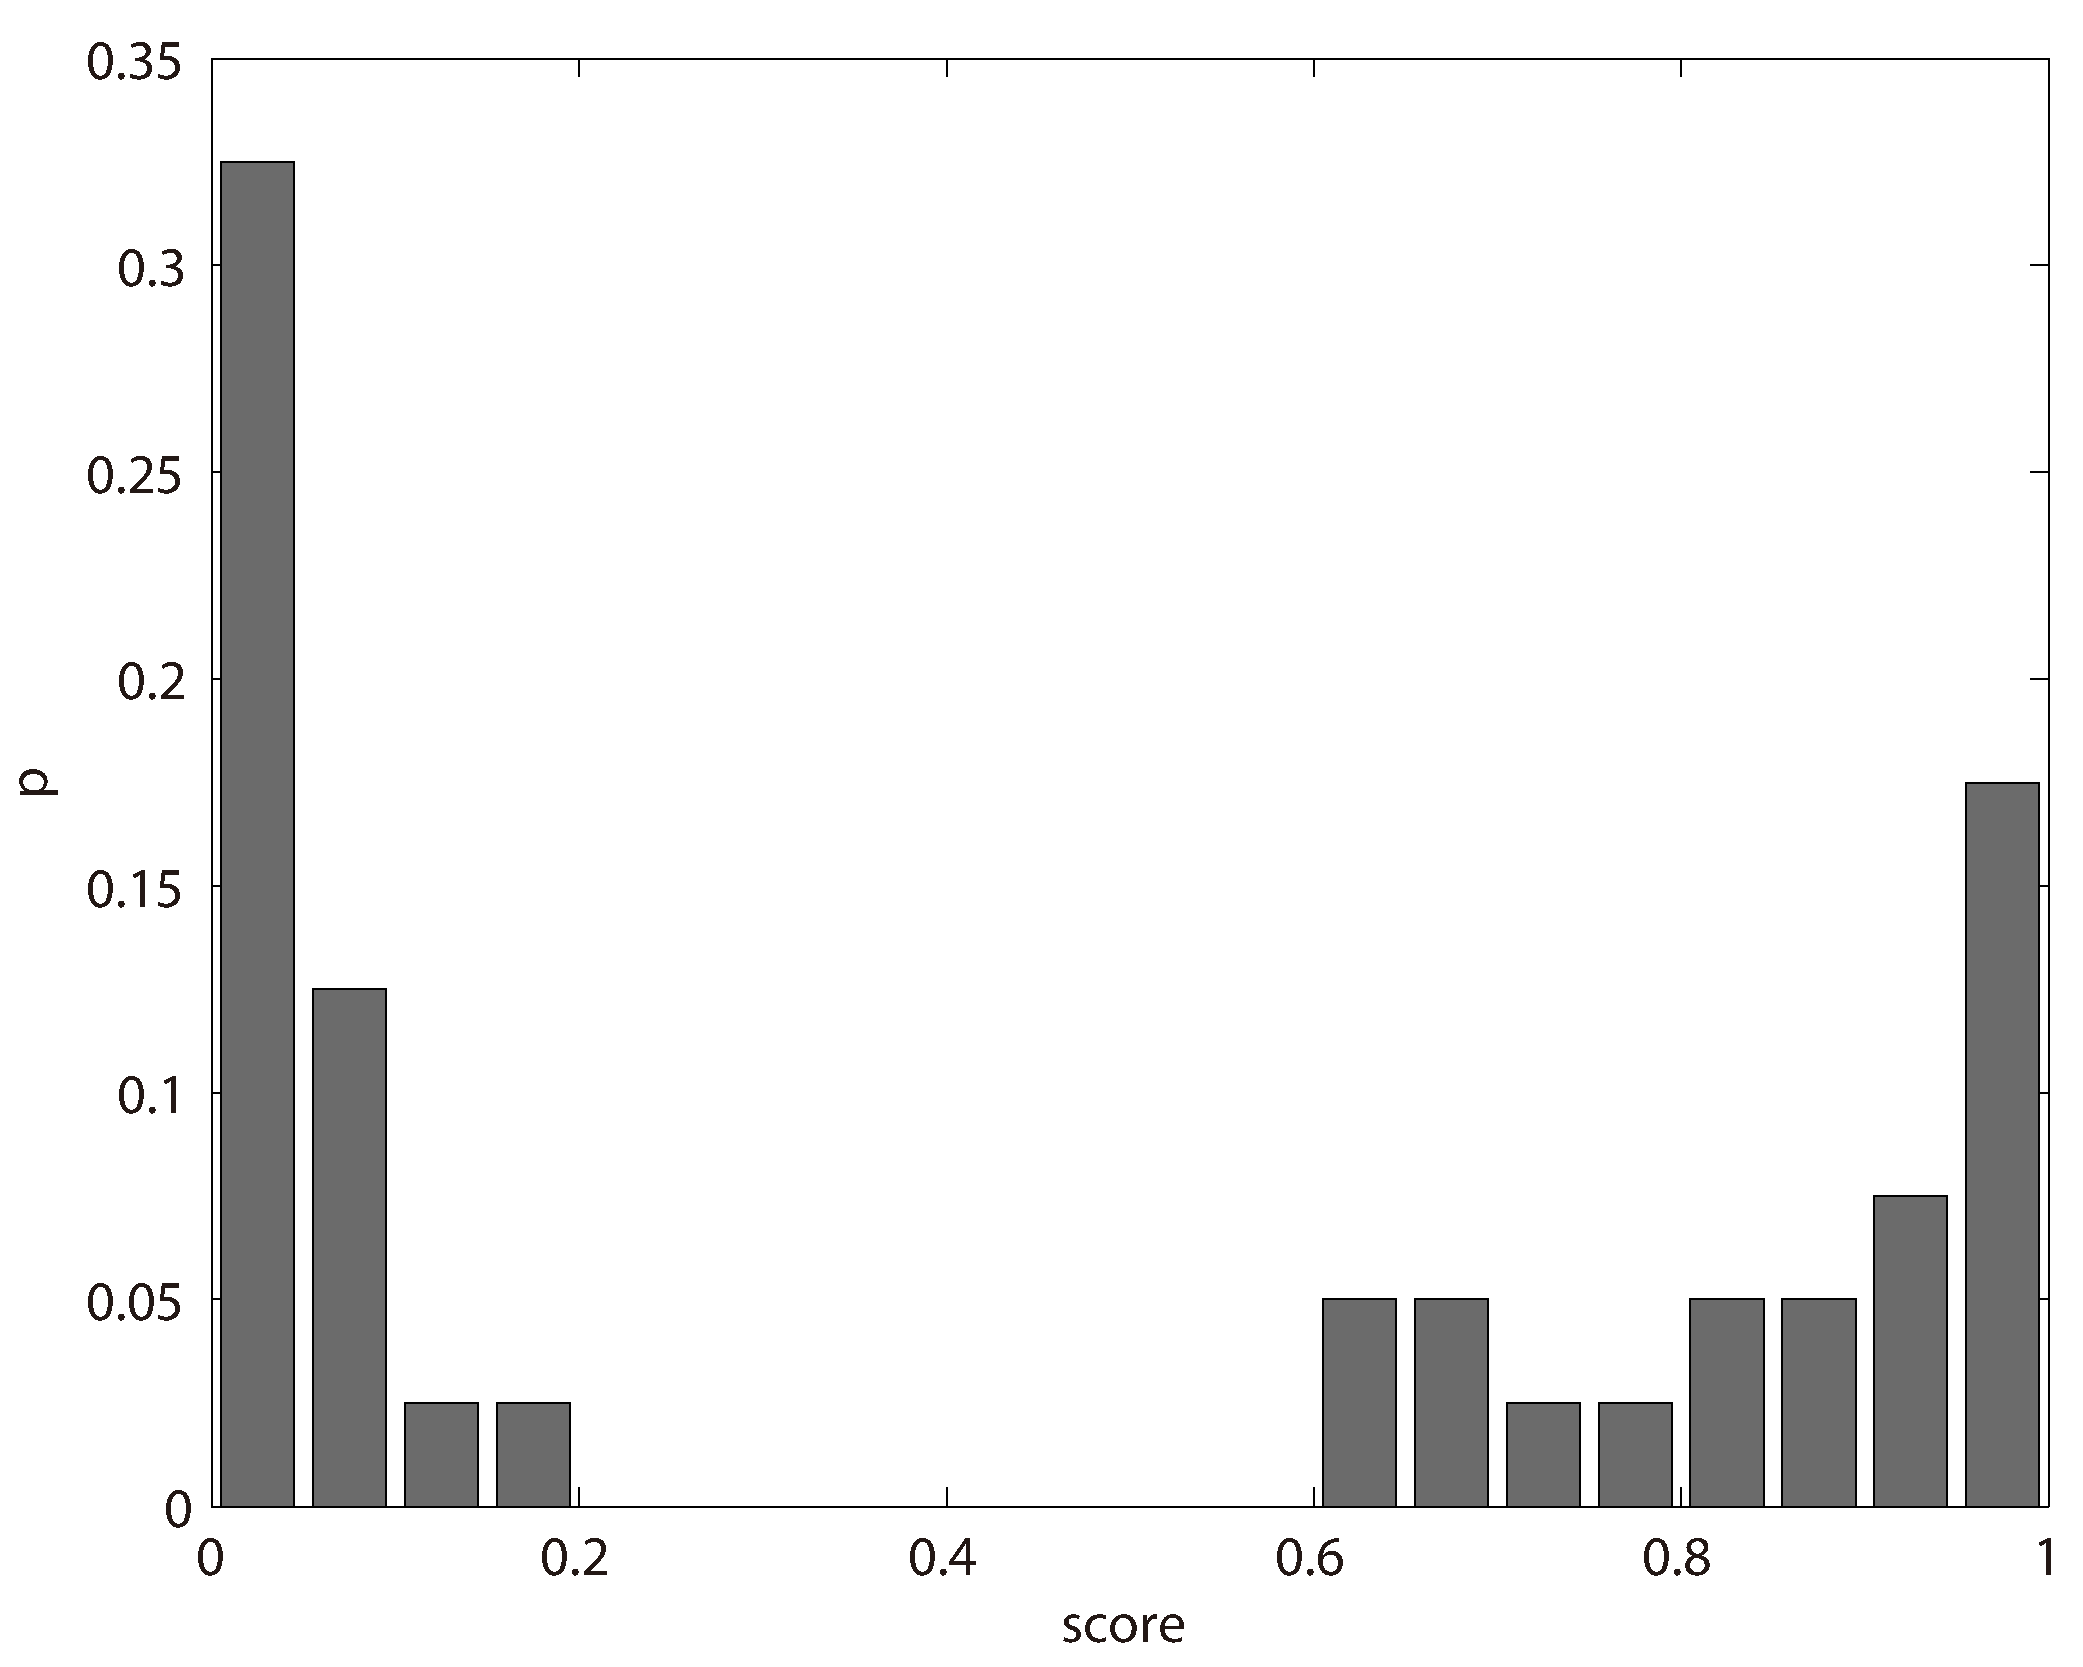
\includegraphics [width=0.7\textwidth]{fig/fig_score.pdf}
  \bicaption[fig:score]{实验页面的评分的频率分布直方图}{实验页面的评分的频率分布直方图。可以看到好坏美感的评分被清晰地二值化分开成了两个具有好坏页面代表性的组别。差的网页的评分的一致性相比好的网页更高,一定程度上证实了人们往往对对象的不美观上更容易达成一致【】}{Fig}{The distribution of the pages on scores. There are clearly two groups. The bad pages are generally more definite, while the good pages are more evenly distributed.}
\end{figure}

\section{分析}
\label{sec:exp1-ana}

\subsection{传统的眼动指标}
首先,对我收集到的眼动数据,我们试验一些传统的描述性指标。这些指标大部分都在第\ref{chap:related}章相关研究中被提及:

\begin{itemize}
  \item 注视总数
  \item 平均注视时长
  \item 注视时长的标准差
  \item 平均扫视距离
  \item 扫视距离的标准差
  \item AOI个数
  \item AOI中注视的平均个数
  \item AOI中注视个数的标准差
\end{itemize}

上面提到的AOI是Area of interests的缩写,表示视觉兴趣点,是通过对页面上捕捉到的所有注视进行空间聚类得到空间区块。我们采用Tobii Studio软件包中自带的默认AOI聚类算法来获得这些AOI区块。图\ref{fig:aoi}以参与实验的一张样本页面为例,标出了它的AOI聚类情况。

\begin{figure}[H]
  \centering
  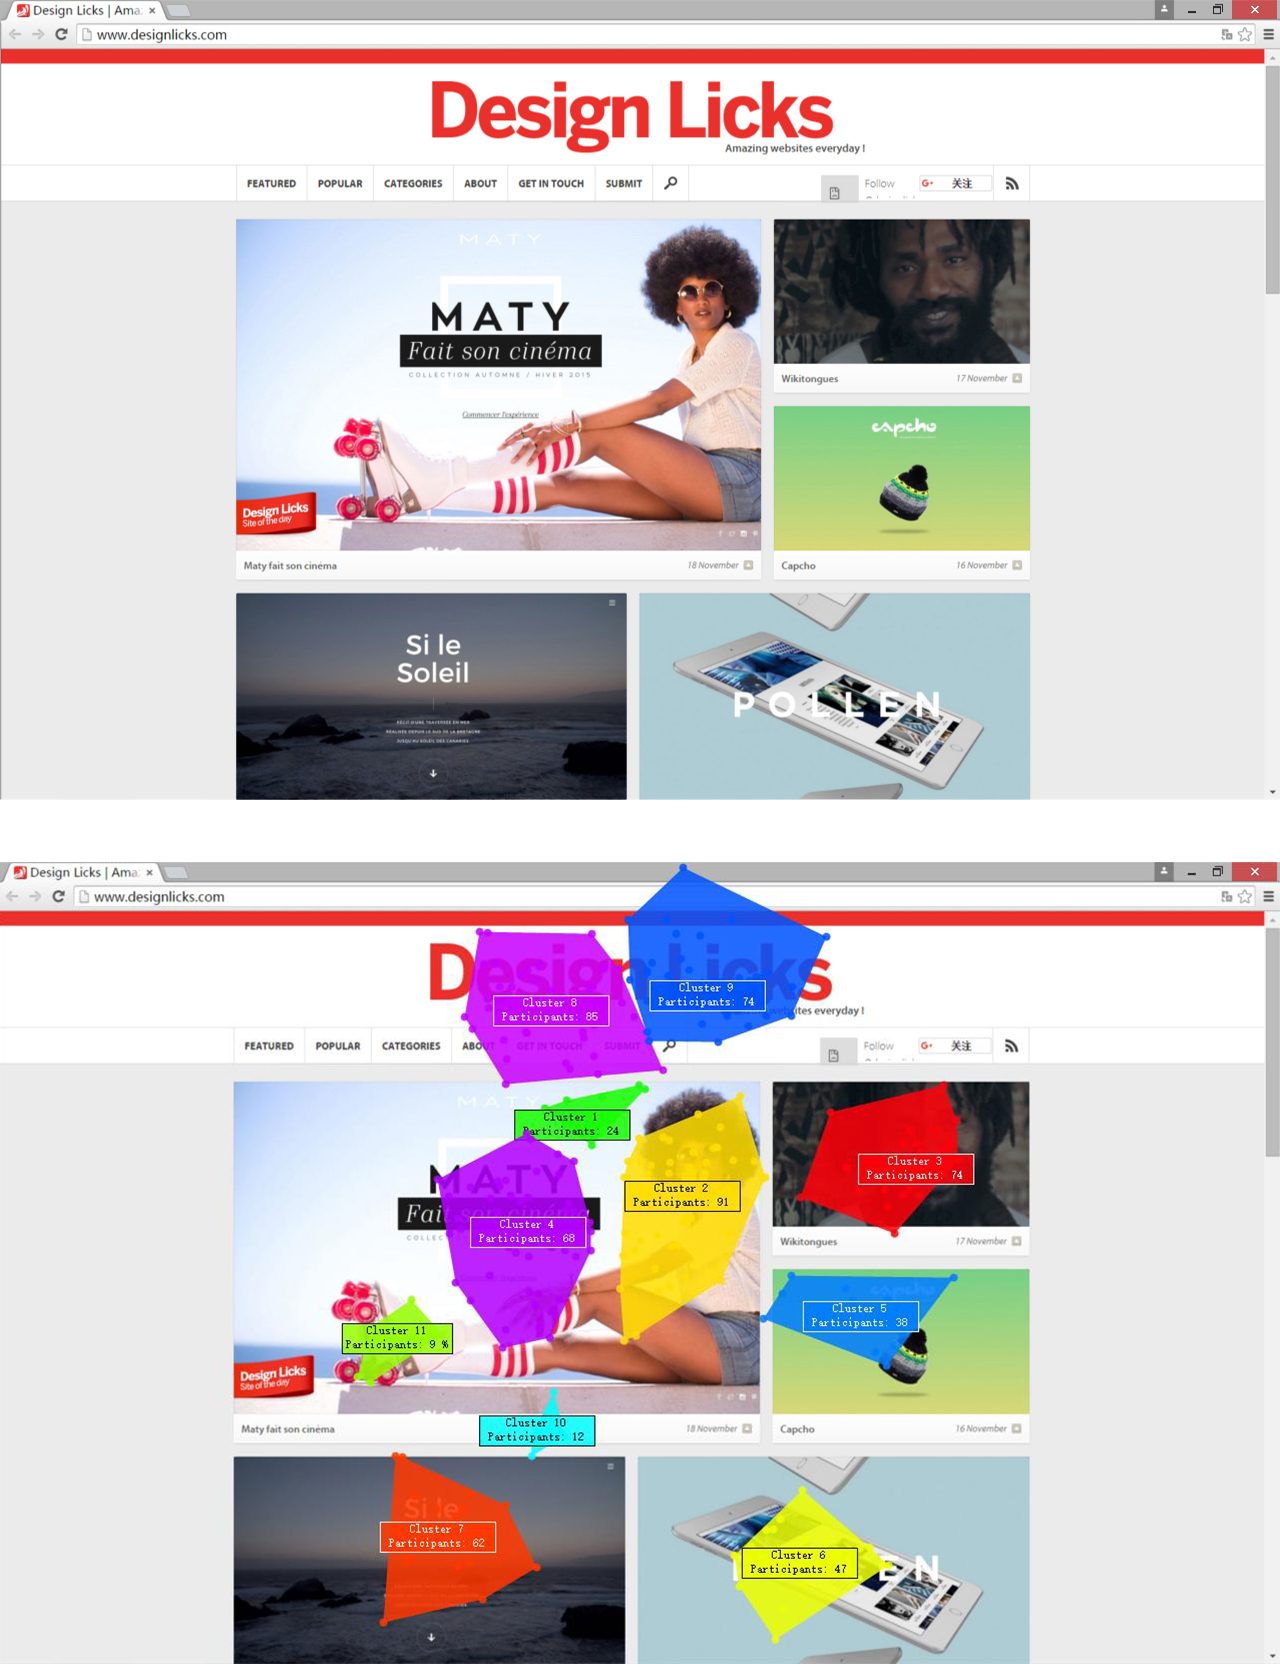
\includegraphics [width=0.85\columnwidth]{fig/fig_AOI.jpg}
  \bicaption[fig:aoi]{AOI聚类的示意图}{AOI聚类的示意图。上方是参与眼动实验的一张页面,下方是该页面与其AOI聚类结果的重叠图。AOI聚类通过Tobii Studio软件自带的聚类算法来实现。该页面一共产生了11个AOI聚类区块。}{Fig}{Top is one of the testing pages. Bottom is the page overlapped with AOIs, which are generated using default clustering tool in Tobii studio. There are total 11 AOIs for this page.}
\end{figure}

表格\ref{tab:traditional}列出了参与计算的所有传统指标在与美感评分的关联性方面的表现,包括每个指标与评分的线性相关系数和对好坏页面组别进行方差分析的p值。在0.05的置信系数上,只有注视个数通过了方差检验($p=0.04$)。注视个数表现出了微弱的与美感评分的正相关性,也即在相同的曝光时间内,好看的页面普遍获得了更多的眼动注视,拥有更活跃的眼动反馈。

\begin{table}[H]
  \centering
  \begin{tabular}{lrr}
    \hline
     &相关系数 & 方差显著性 \\
    \hline
    注视总数 & 0.3322 & 0.0429 \\
    平均注视时长 & -0.1526 & 0.3227 \\
    注视时长的标准差 & 0.1165 & 0.6219 \\
    平均扫视距离 & -0.2203 & 0.0871 \\
    扫视距离的标准差 & -0.1933 & 0.2732 \\
    AOI个数 & -0.2607 & 0.1631 \\
    AOI中注视的平均个数 & 0.3228 & 0.0782 \\
    AOI中注视个数的标准差 & 0.2556 & 0.0991 \\
    \hline
  \end{tabular}
  \bicaption[tab:traditional]{传统的眼动指标与美感关联性的表现}{传统的眼动指标与美感关联性的表现。这些指标都直接提取自注视、扫视和AOI聚类这些常见的眼动度量,只有注视的总数表现出了微弱的方差检验显著性。}{Table}{The performances of some traditional statistics of fixations, saccades and AOIs. Only the number of fixations has a weak correlation with the aesthetic scores and the ANOVA is significant.}
\end{table}


\subsection{眼动过程中的熵}
熵在信息论和热力学中都有定义。概念上,它用来表达一个系统的混乱度、无序程度,或者反过来说对有序性、确定性的缺乏。

本研究中的视觉熵的概念是基于香农的信息熵理论的。信息熵是基于概率空间的一种对不确定性的度量。对一个具有离散的概率空间$\{x_1, ..., x_n\}$和分布$P(X)$和的随机变量$X$,信息熵$H$(希腊大写字母Eta)定义为:

$$H(X)~=~-\sum_{i=1}^n P(x_i)\cdot log_{2}P(x_i)$$

$H(X)$越大,分布$P(x_i)$就更混乱度而不确定,反之则更有更小的不确定性。

接下来我们借助信息熵来分析眼动两个维度:眼动在AOI间的跳转和注视在空间上的分布。

\subsubsection{注视转移中的熵}
最早在Tole et al【】的关于认知负担的研究中把熵的概念引入到眼动数据的分析中。他用熵来描述11名飞行员在执行不同任务时观察行为的变化。该模型在之后也被应用在一项关于驾车时的眼动行为的研究中。【】
Hooge【】使用一种类似的称之为“视觉路径熵”(scan path entropy)的概念来度量对一个特定视觉兴趣点的眼动一致性。

下面我们依照Tole的基于马尔科夫链的视觉熵的定义,分析其与美感评分的关联性。

这种熵描述了眼镜在注视之间转移的确定性。在实验中,注视的位置的概率空间的大小是$1024\times800$,等同于屏幕的分辨率。如此庞大的概率空间使得不同被试之间的眼动序列无法进行比较。对此,Tole的做法是把整个视觉范围人为分割为一些的区域。在本实验中,我们借助系统自动聚类生成的AOI来完成这种区块划分,并考察眼睛在这些AOI间的跳转。跳转是由视觉注意机制所驱动的,在无意识的情况下从当前的目标切换到外围视觉的目标【】,这也就是Berlyne所提出的全面视觉探索的意思。通过AOI对注视的聚类,我们可以将来自原始数据的每个被试的注视跳转转化为AOI之间的跳转(见表\ref{tab:seq})。

\begin{table}[H]
  % \small
  \begin{tabular}{ll}
    1. & 6 - 7 - 11 - 3 - 11 - 10 - 9 - 2 - 3 - 4\\
    2. & 7 - 3 - 4 - 8 - 6 - 4 - 3 - 2\\
    3. & 3 - 5 - 9\\
    4. & 7 - 4 - 8 - 11 - 3 - 7 - 11\\
    5. & 7 - 4 - 8 - 11 - 4 - 7 - 2 - 9\\
    6. & 7 - 3 - 7 - 4 - 8 - 11 - 9 - 2 - 9\\
    7. & 7 - 8 - 4 - 7 - 11 - 2 - 9 - 2 - 3\\
    8. & 3 - 7 - 11 - 10 - 9 - 2 - 9 - 4\\
    9. & 7 - 11 - 2 - 6 - 7 - 8\\
    10.& 4 - 11 - 5 - 2\\
    11.& 7 - 3 - 11 - 4 - 8 - 7 - 2\\
    12.& 7 - 3 - 4 - 8 - 3 - 2 - 9\\
    13.& 6 - 3 - 4 - 8 - 3 - 10\\
    14.& 7 - 3 - 1 - 10 - 11 - 7\\
    15.& 7 - 11 - 8 - 4 - 7 - 8 - 9 - 2 - 6 - 2\\
    16.& 7 - 4 - 8 - 5 - 9 - 2 - 9\\
    17.& 11 - 7 - 11 - 10\\
    18.& 7 - 3 - 4 - 8 - 11 - 10 - 9 - 2\\
    19.& 7 - 11 - 10 - 2 - 9 - 4 - 8\\
    20.& 7 - 4 - 8 - 7 - 3 - 1 - 3\\
    21.& 7 - 11 - 10 - 2 - 9\\
    22.& 7 - 3 - 11 - 10 - 2\\
    23.& 3 - 4 - 1 - 3 - 8 - 4 - 11\\
    24.& 7 - 11 - 4 - 8 - 3 - 9 - 2 - 9\\
    25.& 7 - 4 - 8 - 3 - 2 - 9 - 8 - 4 - 11\\
    26.& 7 - 4 - 8 - 11 - 7 - 3 - 2 \\
    27.& 7 - 3 - 4 - 8 - 11 - 7\\
    28.& 6 - 7 - 8 - 4 - 7 - 8 - 11 - 4 - 2\\
    29.& 7 - 11 - 7 - 3 - 11 - 8 - 4 - 8 - 7\\
    30.& 3 - 7 - 4\\
    \\
  \end{tabular}
  \bicaption{AOI之间的眼动跳转示例}{30个被试的在图\ref{fig:aoi}中的例图的11个AOI之间的眼动跳转序列}{Table}{Gaze transitions of the 30 subjects among the 11 AOIs in the image (see Figure \ref{fig:aoi}).}
\end{table}

\paragraph{眼动的马尔科夫性}
如果一个离散时间序列 $X_1,X_2,X_3,...$ 满足$P(X_{n+1}=x~|~X_1=x_1,X_2=x_2,...,X_n=x_n)~=P(X_{n+1}=x~|~X_n=x_n)$),则称之为一个离散马尔科夫链。对于眼动的AOI序列,其马尔可夫性可以简单地解释为下一个注视的AOI只与当前注视的AOI有关。

对于一个马尔科夫序列,其全部的转移概率信息可以通过一个一步转移概率矩阵来表示。

在假设眼动的马尔可夫性成立的前提下,实验中的一个页面上的AOI之间的一步转移概率可以通过统计其在被试的眼动数据中的出现的概率来获得。表\ref{tab:mat}中展示了\ref{fig:aoi}中举例页面的11个AOI之间的一步转移概率矩阵:

\begin{table}[H]
\centering
  \begin{tabular}{@{}lllllllllll@{}}
  \hline
  0    & 0    & 0.67 & 0    & 0    & 0    & 0    & 0    & 0    & 0.33 & 0    \\
  0    & 0    & 0.14 & 0    & 0    & 0.14 & 0    & 0    & 0.71 & 0    & 0    \\
  0.08 & 0.16 & 0    & 0.28 & 0.04 & 0    & 0.16 & 0.04 & 0.04 & 0.04 & 0.16 \\
  0.04 & 0.04 & 0.04 & 0    & 0    & 0    & 0.15 & 0.63 & 0    & 0    & 0.11 \\
  0    & 0.33 & 0    & 0    & 0    & 0    & 0    & 0    & 0.67 & 0    & 0    \\
  0    & 0.17 & 0.17 & 0.17 & 0    & 0    & 0.5  & 0    & 0    & 0    & 0    \\
  0    & 0.05 & 0.3  & 0.22 & 0    & 0    & 0    & 0.14 & 0    & 0    & 0.3  \\
  0    & 0    & 0.17 & 0.26 & 0.04 & 0.04 & 0.13 & 0    & 0.04 & 0    & 0.3  \\
  0    & 0.73 & 0    & 0.2  & 0    & 0    & 0    & 0.1  & 0    & 0    & 0    \\
  0    & 0.43 & 0    & 0    & 0    & 0    & 0    & 0    & 0.43 & 0    & 0.14 \\
  0    & 0.1  & 0.1  & 0.17 & 0.04 & 0    & 0.21 & 0.08 & 0.04 & 0.29 & 0\\
  \hline
  \end{tabular}
\bicaption[tab:mat]{AOI之间的一步转移概率矩阵示例}{例图的11个AOI之间的一步马尔科夫转移概率矩阵}{Table}{Markov transition probability matrix of the 11 AOIs.}
\end{table}

矩阵中,$p_ij$表示在当前注视在视觉兴趣点i的前提下,跳转到视觉兴趣点j的转移概率。

在此转移概率矩阵的基础上,眼动熵如下定义

$$H = \sum_{i=1}^n(P(i)\sum_{j\neq i} p_{ij}log_2(p_{ij}))$$

其中$p_{ij}$表示从视觉兴趣点$i$跳转到视觉兴趣点$j$的条件概率。$p(i)$表示注视在视觉兴趣点$i$上的先验概率,即从视觉兴趣点$i$开始进行下一步跳转的概率,通过统计视觉兴趣点i被注视到的概率来估计。
极大熵$H_{max}$表示在一个页面的AOI个数的前提下,可能出现的最大视觉转移熵。可以通过假设所有的先验概率和转移概率都相等来获得。用上述的视觉熵除以极大熵获得的相对视觉熵令不同的页面之间的结果具有可比性。

$$H_{relative}~=~\frac{H}{H_{max}}$$

上述的视觉熵可以度量视觉兴趣点之间一次转移的确定性。我们期望美感评分高的页面相对低的页面会有更小的视觉熵。然而结果是令人失望的。基于我们的3秒钟曝光的眼动数据,熵与美感评分间的线性相关系数只有0.1585,好坏两类之间的方差检验的$p=0.4741$。

\begin{table}[H]
\centering
\begin{tabular}{lrrrrr}
  \hline
  Source&SS&df&MS&F&Prob$>$F\\ \hline
  Groups&0.00166&1&0.00166&0.52&0.4741\\
  Error&0.12101&38&0.00318&&\\
  Total&0.12268&39&&&\\
  \hline
\end{tabular}
\bicaption[tab:ANOVA-ve]{基于AOI转移的视觉熵的方差分析}{基于AOI转移的视觉熵的方差分析}{Table}{ANOVA of visual entropy based on the gaze transitions.}
\end{table}

对于上述眼动熵与美感没有显著关联性的可能是如下两个原因导致的如下:

\begin{itemize}
  \item 统计一次的马尔科夫转移跳转的熵的模型可能过于简化了,然而通过更多转移步长将大大减少可用于概率估计的数据量。
  \item AOI的聚类算法可能丢失了一些信息并产生了一些AOI的不合理聚类。
\end{itemize}

\subsubsection{基于热图的熵}
上述的基于马尔科夫链的熵把眼动行为理解成由注视和扫视(转移)构成的一系列相关事件。
这里我们引入一种新的基于最广泛应用在眼动数据中的可视化手段【Nielsen2010】——热图的熵的概念。与之前用来计算熵的眼动转移序列不同,热图没有包含任何有关注视顺序的信息,这意味着新的熵度量是独立看待所有的眼动注视的。

\begin{figure}[H]
  \centering
  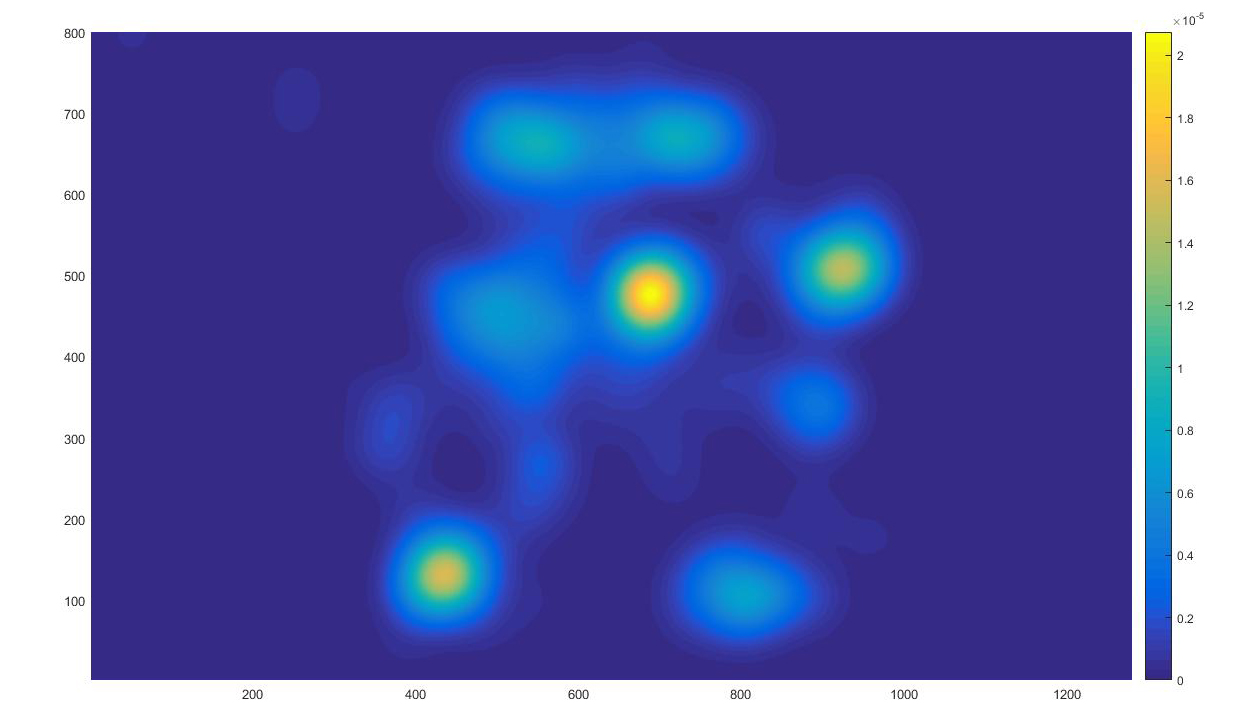
\includegraphics [width=\columnwidth]{fig/fig_eg_hm.jpg}
  \bicaption[fig:hm]{眼动热图示例}{图\ref{fig:aoi}中的例图的眼动热图。它是对眼睛在画面上的注视位置的概率分布的一种逼近或估计。}{Fig}{The heatmap of the example pages in figure \ref{fig:aoi}. It visualizes the spatial probability distribution of fixations on the page.}
\end{figure}

考察代表眼动注视的位置的二维随机变量$(X, Y)$,则它的概率空间就是屏幕的分辨率空间(即把屏幕上的每一个像素认为是注视的一种可能的位置选择)。基于作用在该随机变量上的概率分布$P(X, Y)$,可以如下定义熵:

$$H(P)~=-\sum_{i=1}^{1280} \sum_{j=1}^{800} P(x_i, y_j)log_2(P(x_i, y_j))$$
其中: $$\sum_{i=1}^{1280}\sum_{i=1}^{800}~P(x_i, y_j)~=~1$$

而$(X, Y)$的概率分布$P(X, Y)$,实际上就是眼动热图,可以通过眼动数据进行估计。
热图的这种熵可以反映被试的眼动在空间上的分布的一致性或者凝聚度:当所有的注视聚焦在同一个像素上时,产生最小的熵值、让所有的注视平均地分散在屏幕上时,产生最大的熵值。
通过引入高斯核对每个注视点在空间上进行模糊处理,可以实现用少量的眼动采样据来估计注视在屏幕上的空间分布。
对一个屏幕横坐标位置为$x_0$,纵坐标位置为$y_0$,持续时长为$d$的眼动注视,它产生的高斯核可以表达为

$$d\cdot e^{-\frac{(x-x_0)^2 + (y-y_0)^2}{2\sigma^2}}$$

其中$\sigma$是高斯核的标准差。注意到上述的表达式并非标准的归一化的正态分布表达式,因为最终通过这些高斯核叠加得到的分布$P(X, Y)$还要进行归一化处理,以满足$\sum\sum P(X, Y) = 1$
除了用有限数据估计概率分布的需要之外,引入高斯核叠加的合理性还体现在人眼的注视事实上是与人眼的黄斑对应的具有一定半径的圆形范围,而实际的眼动注视也并非绝对固定不动而是包含一些微动行为的【】。另外考虑到眼动仪的检测本身具有一定的误差范围,高斯叠加的做法也令指标对误差具有一定的容忍度。\ref{fig:hm}展示了$\sigma=30px$时的热图的形态。
通过对40张实验页面的热图的熵的计算,发现其与美感评分表现出显著的负相关性($r = -0.5412, ANOVA F = 15.79 P = 0.0003$)。

\begin{table}[H]
\centering
\begin{tabular}{lrrrrr}
  \hline
  Source&SS&df&MS&F&Prob$>$F\\ \hline
  Groups&1.15861&1&1.15861&15.79&0.0003\\
  Error&2.78901&38&0.07339&&\\
  Total&3.94762&39&&&\\
  \hline
\end{tabular}
\bicaption[tab:ANOVA-vae-dw]{VAE的方差分析}{热图熵(视觉注意熵)的方差分析。}{Table}{ANOVA analysis of the entropy of heatmap.}
\end{table}

到目前为止,基于热图的熵是与美感表现出最强相关性的指标。鉴于热图有时会被认为是视觉注意的分布图,我们把上述定义的基于热图的熵称作视觉注意熵(Visual Attention Entropy,VAE)。


\subsection{相对VAE}
对于上面得到的VAE指标,存在着一定的理论缺陷。视觉注意熵与美感评分是负相关的,然而一个绝对低的VAE值并不意味着一个相当高的美感评分:一个只拥有相当少的内容的页面可能会得到一个相当低的VAE值,反之一个铺满内容的页面可能有相当高的VAE值,但显然这并不意味着前者一定比后者好看。理论上,具有不同内容复杂度的页面之间是无法通过VAE进行比较的。
为了解决该问题,我们引入了我们称之为相对VAE(relative, rVAE)的概念。为了让不同的页面的VAE可比较,需要首先考察他们各自的基础视觉注意熵(base VAE, bVAE)。对于一个页面,bVAE通过统计所有的被试各自的VAE的平均值得到,代表着一个无噪声扰动的VAE情况,是该页面的必要视觉注意成本。

$$bVAE~=~\frac{1}{n}\sum_{i=1}^n VAE(P_i)$$

其中n是被试人数,$VAE(P_i)$表示第i个被试的个体眼动注意熵。以bVAE作为一个先决条件,可以定义如下的相对视觉注意熵rVAE:

\begin{equation}
rVAE = \frac{VAE}{bVAE}
\label{formula:rvae}
\end{equation}

与VAE相比,rVAE与美感评分的关联性有显著提高,线性相关系数从-0.54提高到了-0.66。$ANOVA F = 26.84 P = 0.000008$。

\begin{table}[H]
\centering
\begin{tabular}{lrrrrr}
  \hline
  Source&SS&df&MS&F&Prob$>$F\\ \hline
  Groups&0.00336&1&0.00336&26.84&7.53E-06\\
  Error&0.00475&38&0.00013&&\\
  Total&0.00811&39&&&\\
  \hline
\end{tabular}
\bicaption[tab:ANOVA-rvae-dw]{rVAE的方差分析}{相对视觉注意熵(rVAE)的方差分析}{Table}{ANOVA of rVAE.}
\end{table}

\ref{formula:rvae}似乎表明,基础视觉注意熵(bVAE)越大则相对视觉注意熵(rVAE)越小,则对应的美感有越大可能更好。但事实上,这不完全正确,由于之间的显著的相关性($r = 0.77$)表\ref{tab:corr},拥有较高的bVAE的页面很可能也会有较高的VAE。如果把bVAE当做是---

\begin{table}[H]
\centering
\begin{tabular}{l|rrrrrr}
  \hline
        &美感评分&注视总数&VAE&bVAE&rVAE\\ \hline
  美感评分 &1&0.33&\bfseries{-0.54}&-0.13&\bfseries{-0.66}\\
  注视总数&-&1&0.14&\bfseries{0.61}&-0.14\\
  VAE&-&-&1&\bfseries{0.77}&\bfseries{0.94}\\
  bVAE&-&-&-&1&0.52\\
  rVAE&-&-&-&-&1\\
  \hline
\end{tabular}
\bicaption[tab:corr]{重要眼动指标的相关系数}{主要的眼动指标和美感得分两两之间的相关系数。}{Table}{The pearson correlations in-between the aesthetic scores and the main indices.}
\end{table}

上述关键指标间的相关性分析表明,bVAE与美感评分几乎没有相关性,但与注视的个数有较为显著的相关性。图\ref{fig:bvae}列出了所有的页面的个体VAE的盒图。

\begin{figure}[H]
  \centering
  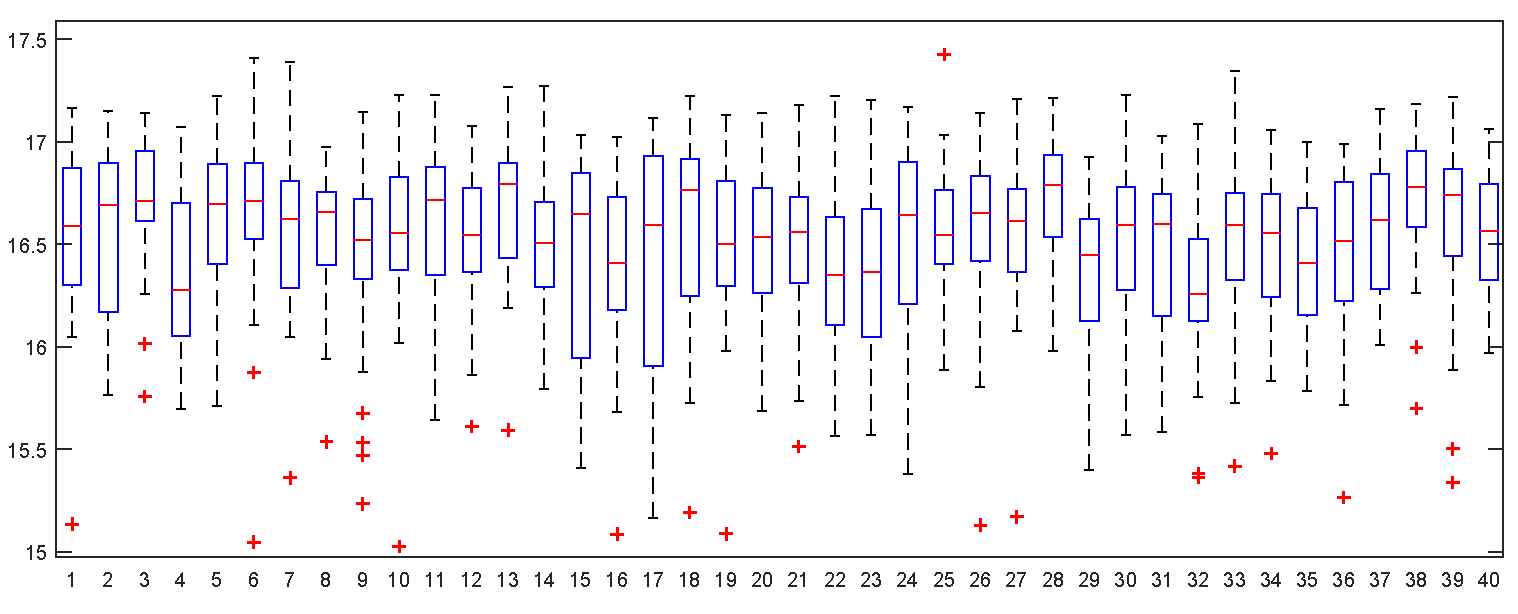
\includegraphics [width=1\columnwidth]{fig/fig_bvae.pdf}
  \bicaption[fig:bvae]{bVAE的盒图}{40张页面上30个被试的视觉重点熵(VAE)的盒图。页面从做到右按照美感评分排序。红色短横线代表均值,及该页面的基础视觉注意熵(bVAE)。在好坏页面见没有表现出显著差异。}{Fig}{Boxplots of the 30 individual VAEs on each of the 40 webpages. The 40 pages are sorted by their scores, from low to high. The red lines in the boxes represent the bVAEs (means).  There is no apparent difference between the good and the bad pages}
\end{figure}

bVAE的引入使得具有不同内容复杂度的页面的VAE变得可比较,并提供了对他们的美感评分的更为精确的预测。
图\ref{fig:box}展示了VAE和rVAE的方差分析盒图。展示了所有40张实验页面的美感评分分别关于VAE和rVAE的散点图。相比VAE,rVAE在区分好坏页面上具有更好的表现。

\begin{figure}[H]
  \centering
  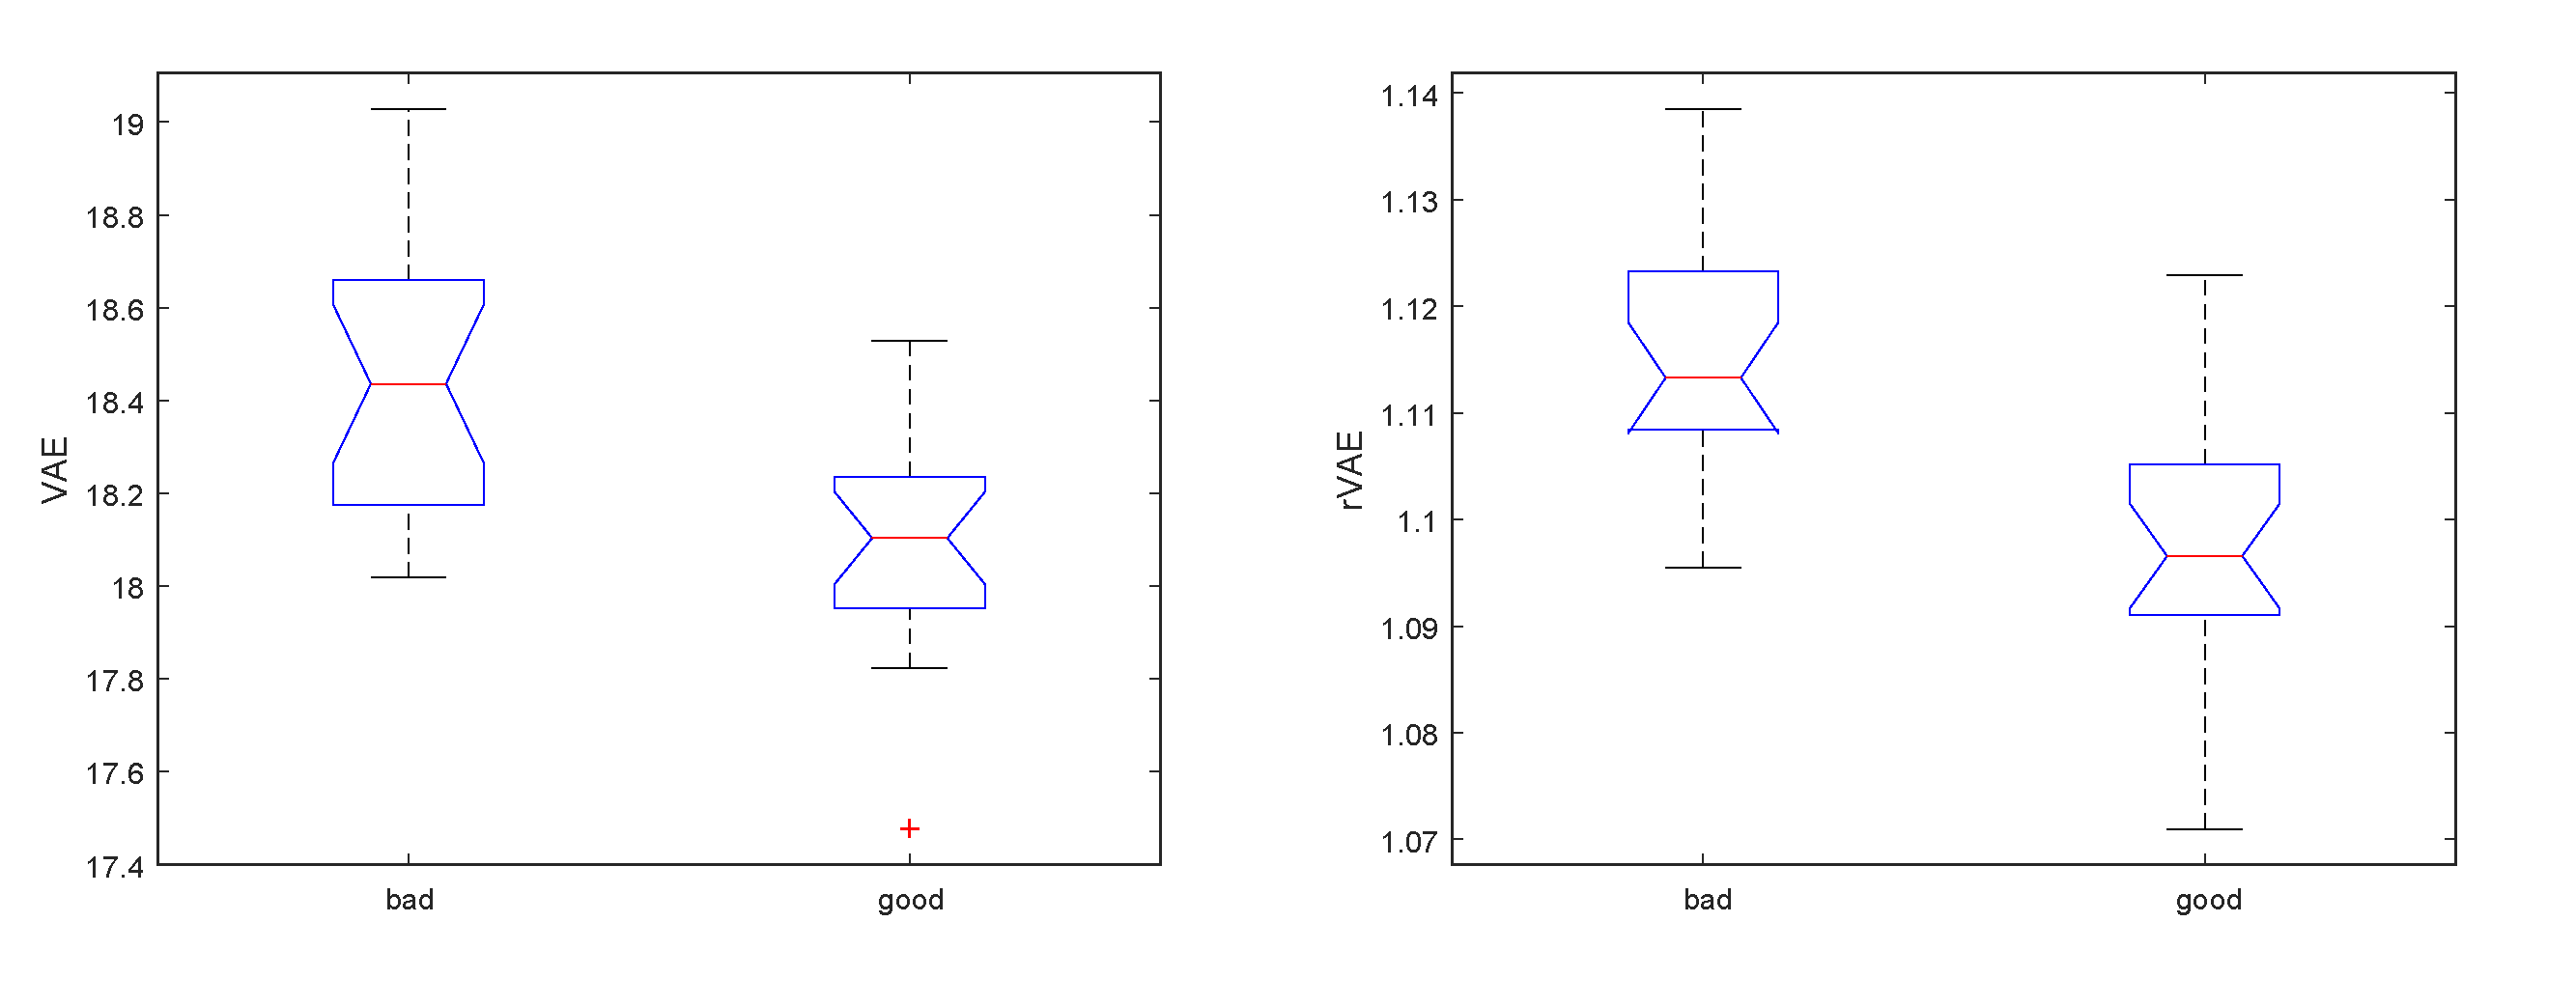
\includegraphics [width=1\columnwidth]{fig/fig_box.pdf}
  \bicaption[fig:box]{VAE和rVAE的盒图}{VAE和rVAE的盒图。左为VAE右为rVAE。显然,rVAE更显著地区分了好坏两个页面组别。}{Fig}{Boxplot of VAE (left) and rVAE (right). Apparently, the rVAEs more significantly separate the two classes.}
\end{figure}

\begin{figure}[H]
  \centering
  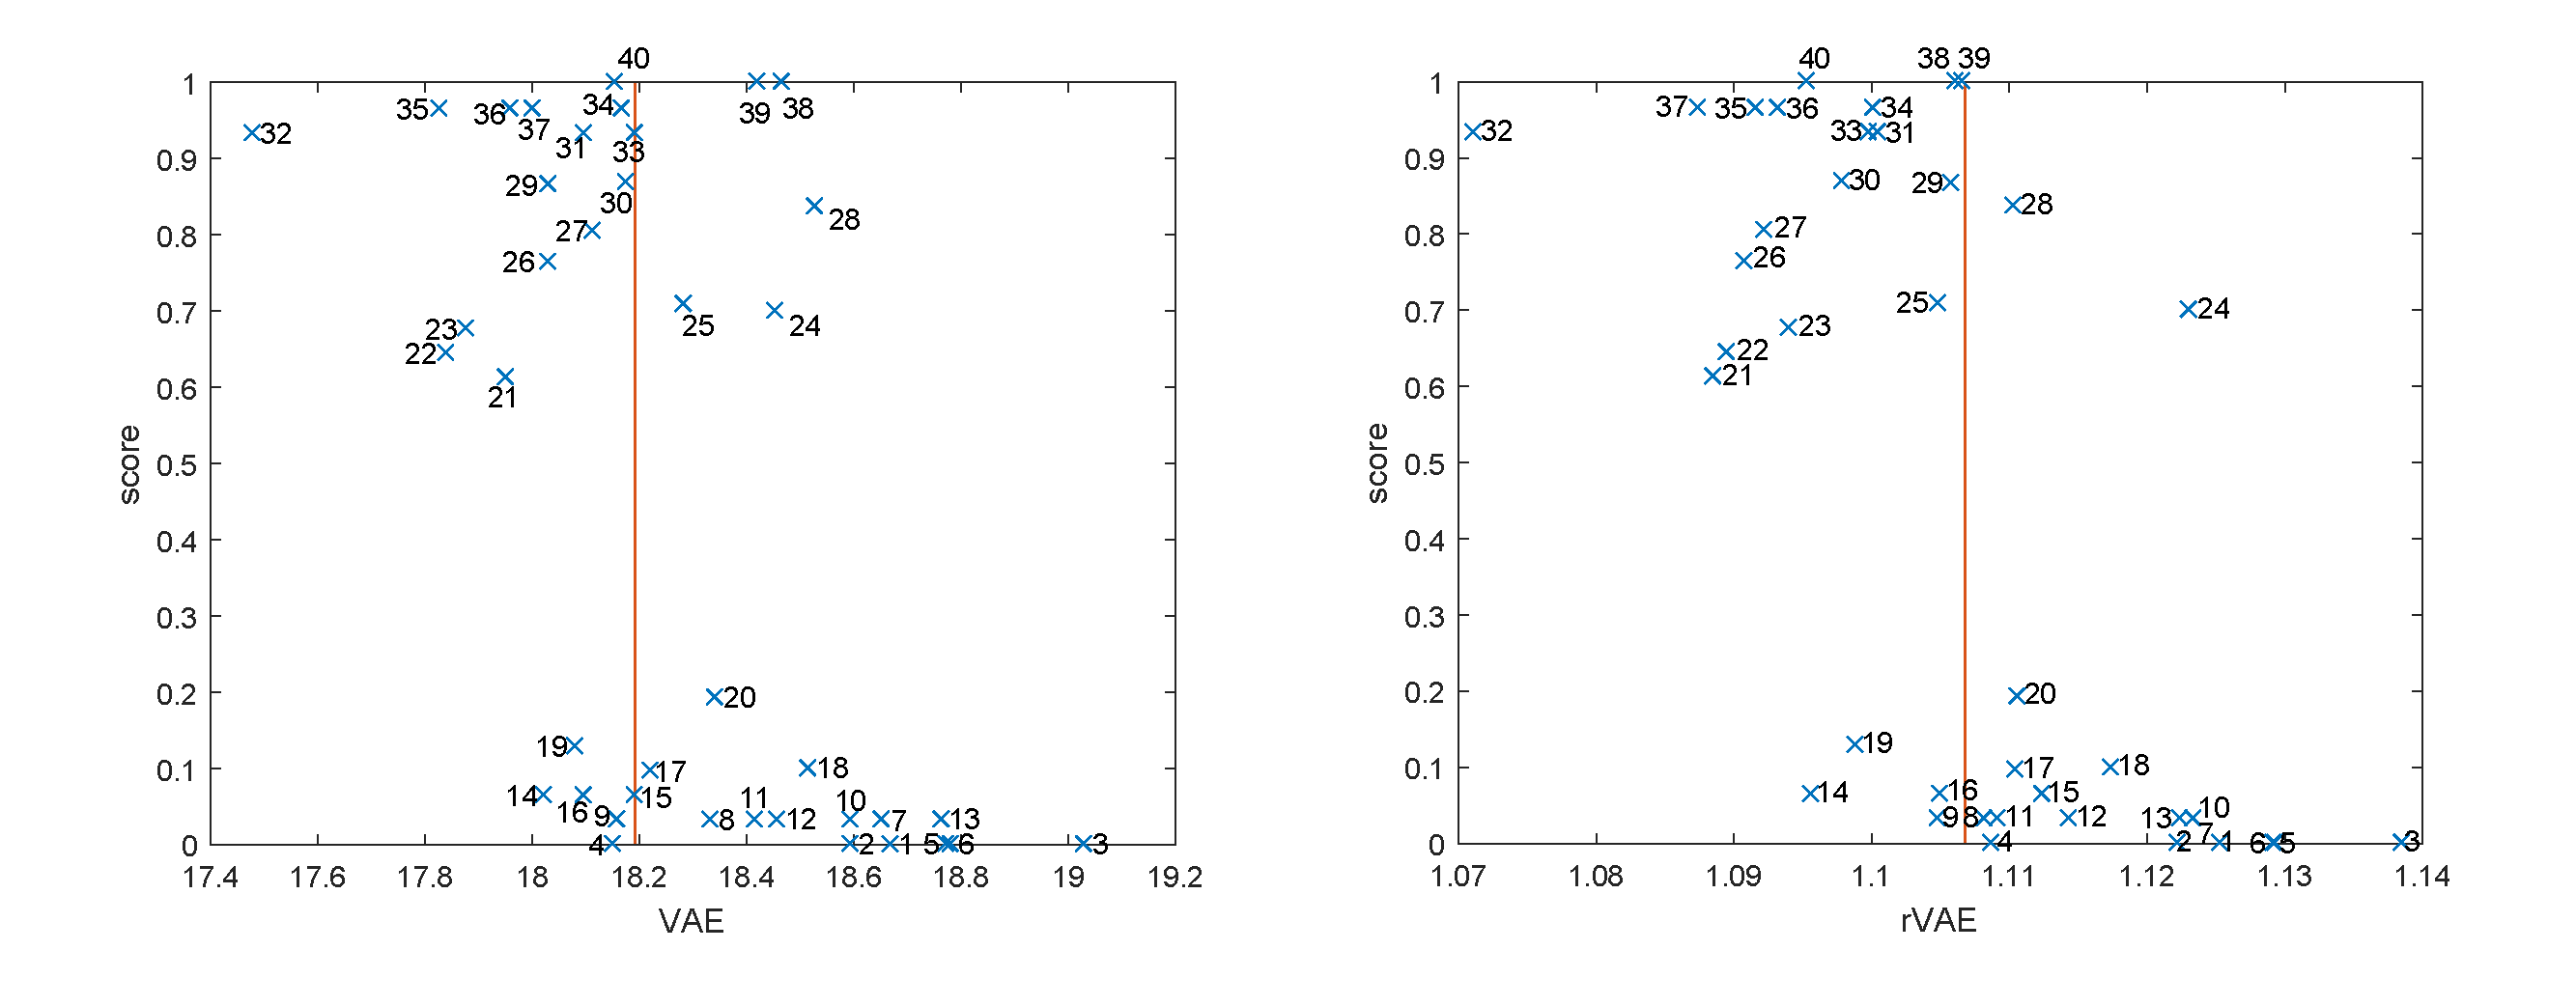
\includegraphics [width=1\columnwidth]{fig/fig_with-score.pdf}
  \bicaption[fig:with-score]{VAE和rVAE关于得分的的散点图}{40张页面的VAE-得分散点图(左)和rVAE-得分散点图(右)。右图的点云更强的方向性。}{Fig}{The scatter plots of 40 pages over VAE (left) and rVAE (right). The point cloud in the right plot appears more significantly skewed.}
\end{figure}

\section{例外}
比较图\ref{fig:out}中的两张散点图我们发现总体而言相比VAE,rVAE使得好坏两组页面分得更开了,然而仍有一些被勿分类的页面。一个标注为24号的页面从整体的趋势中明显脱离,它有不错的美感评分,却在VAE和rVAE上都比较高。

图\ref{fig:out}上给出了这张页面的原始样本,不得不承认这张页面看起来还是不错的,包含了很多富有吸引力的因素如:漂亮的图片、色彩、平衡的布局等等。然而从一个设计师的角度,它还有不小的提升空间。全屏来看这张页面时,眼睛会感到一定的选择压力。这可能是因为视觉外围的一些密集的高对比造成的。图\ref{fig:out}下给出了这张页面经过细微版式调整后的版本。它阐明了细微的细节改动是如何改变给人的第一印象的。VAE本质上是受画面的边缘对比、复杂度等底层低级特征影响的,因而我们相信它能够表现观察者的视觉不适。可以肯定的是,我们通过VAE进行度量的视觉注意的流畅性美感判断具有不小的影响力。当然它也并非美感的全部。

\begin{figure}[H]
  \centering
  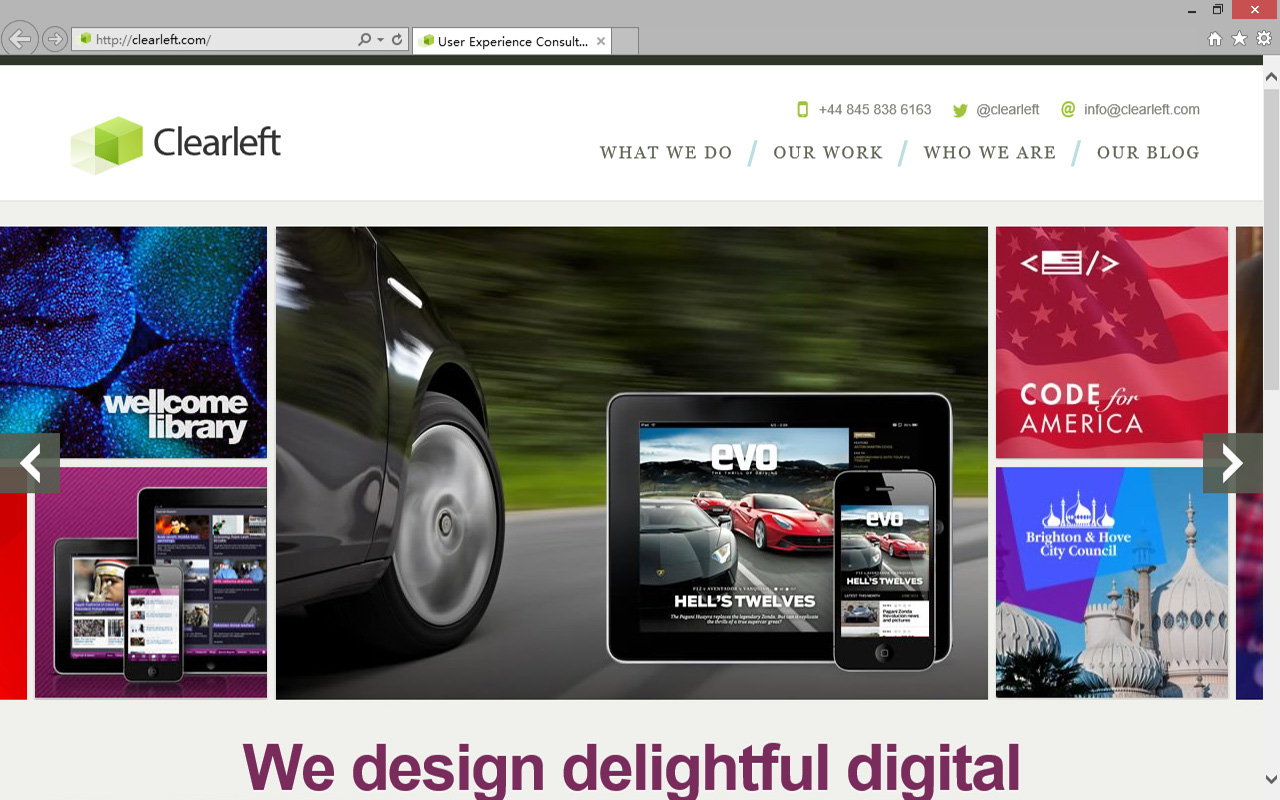
\includegraphics [width=\columnwidth]{fig/fig_out.jpg}
  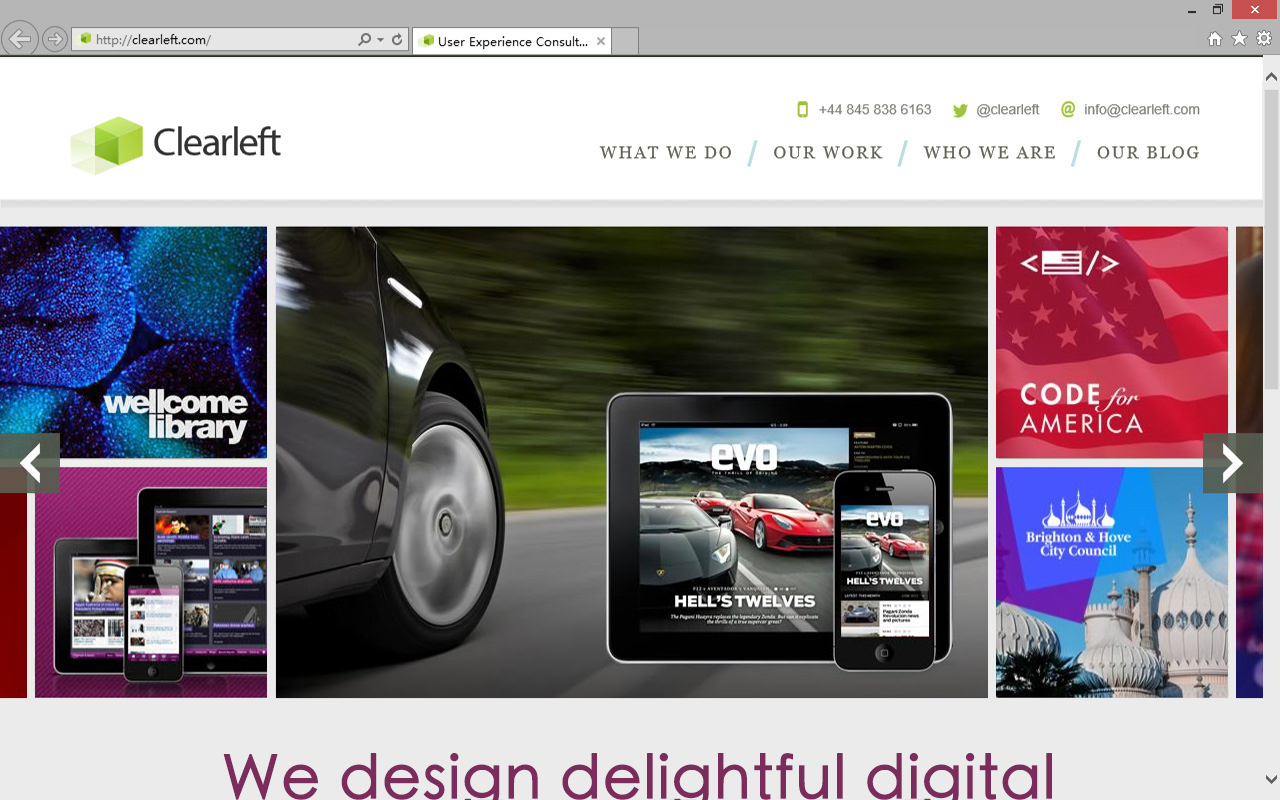
\includegraphics [width=\columnwidth]{fig/fig_out_alt.jpg}
  \bicaption[fig:out]{眼动实验中例外的页面}{例外页面图(上)和改进的例外页面(下)。该页面在图\ref{fig:with-score}中标号24。如果全屏显示,你会觉得视觉上有一些决策压力。 右侧是略微改进后的版本,一些局部的视觉重点被调整了,从而视觉压力略微降低。}{Fig}{The left is one of the outlier pages (point 24 in figure \ref{fig:with-score}). If you display it on full screen, you may feel your eyes a little strained with selection pressure. As a comparison, the right is a revised version, in which some local saliencies have been adjusted. You may feel your eyes slightly relaxed.}
\end{figure}

\section{VAE的稳定性}
为了优化VAE的表现,我们分别考察熵与美感的相关性随着实验时间、纳入计算的被试人数以及热图高斯核的标准差的变化。
对给定的时刻t,我们统计发生在0-t时间段的眼动注视,并基于此计算VAE和rVAE,由此得到VAE和rVAE分别关于时间的变化的曲线。所有的曲线在开始时都表现出了较大幅的波动,然后逐步趋于稳定和平缓。图\ref{fig:with-t} 表现了实验页面的VAE随时间增大,rVAE随时间减小的趋势。
蓝色的曲线代表美感评价好的网页而红色的曲线代表美感评价坏的网页。显然好的页面随时间持续地有更小的VAE和rVAE值。此外在最后的时刻好坏的两个类别分的更开了。

\begin{figure}[H]
  \centering
  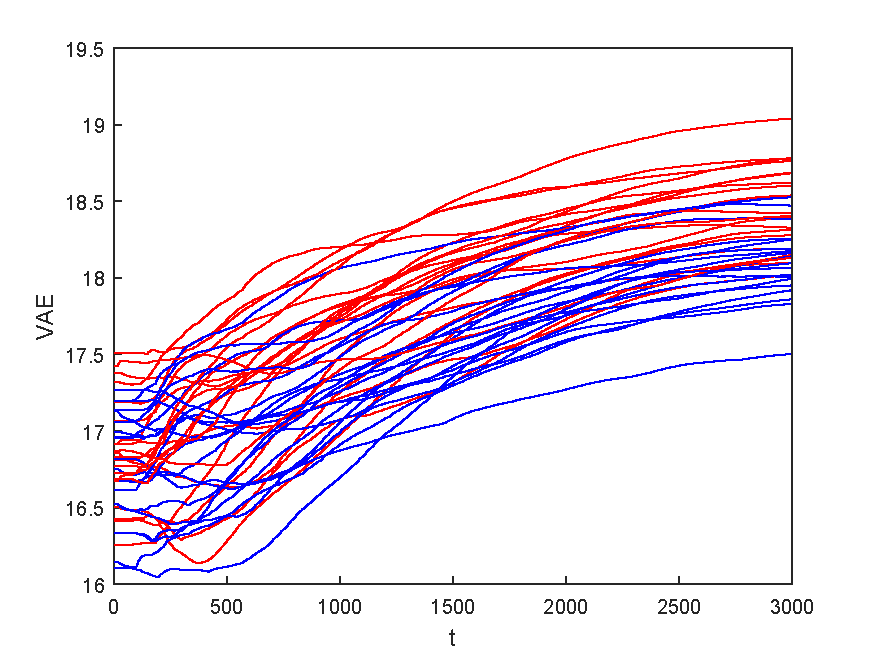
\includegraphics [width=0.85\columnwidth]{fig/fig_vae-t.pdf}
  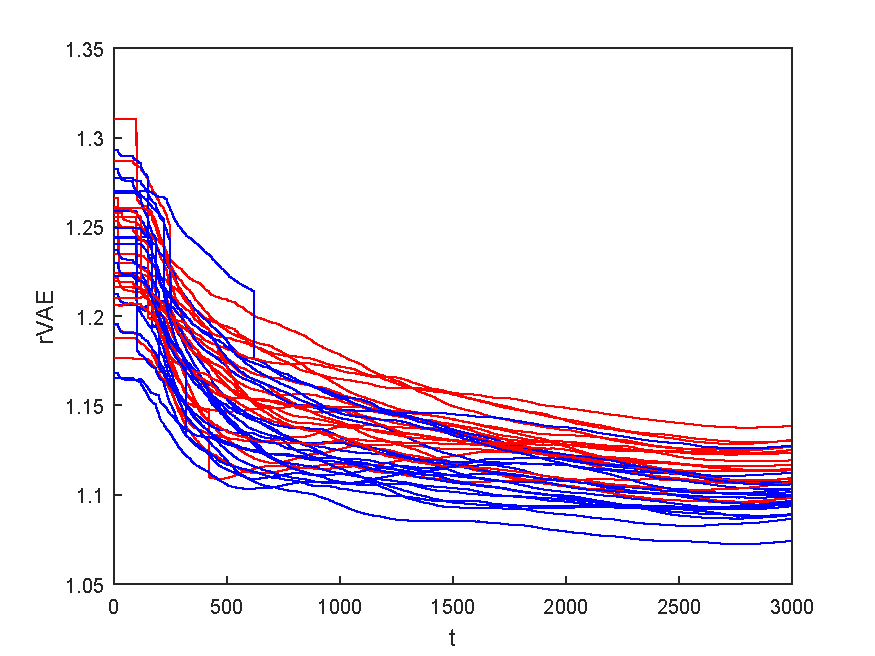
\includegraphics [width=0.85\columnwidth]{fig/fig_rvae-t.pdf}
  \bicaption[fig:with-t]{VAE和rVAE的值随时间的变化}{40张页面的VAE(上)和rVAE(下)随时间的变化图。蓝色曲线代表美感评分较好的网页组别,红色代表坏的。这些曲线随时间逐步趋于稳定,好的页面普遍给出了更小的VAE和rVAE值。两个组别随时间愈发分离。}{Fig}{The VAEs (top) and the rVAEs (bottom) of the 40 pages gradually stabilize over time. The blue curves represent the "good" pages. The red curves represent the "bad" pages. The good pages generally yield lower VAE and rVAE values. The two groups  become more separated towards the end.
}
\end{figure}

图\ref{fig:corr-t}展现了熵和美感评分的相关系数随时间变化的曲线,在三秒的时刻相关系数取得了极值。由于我们没有记录3秒后的眼动数据,故没有办法看到后续的发展趋势。以母线的增长趋势,我们猜测相关系数可以变得更强。

\begin{figure}[H]
  \centering
  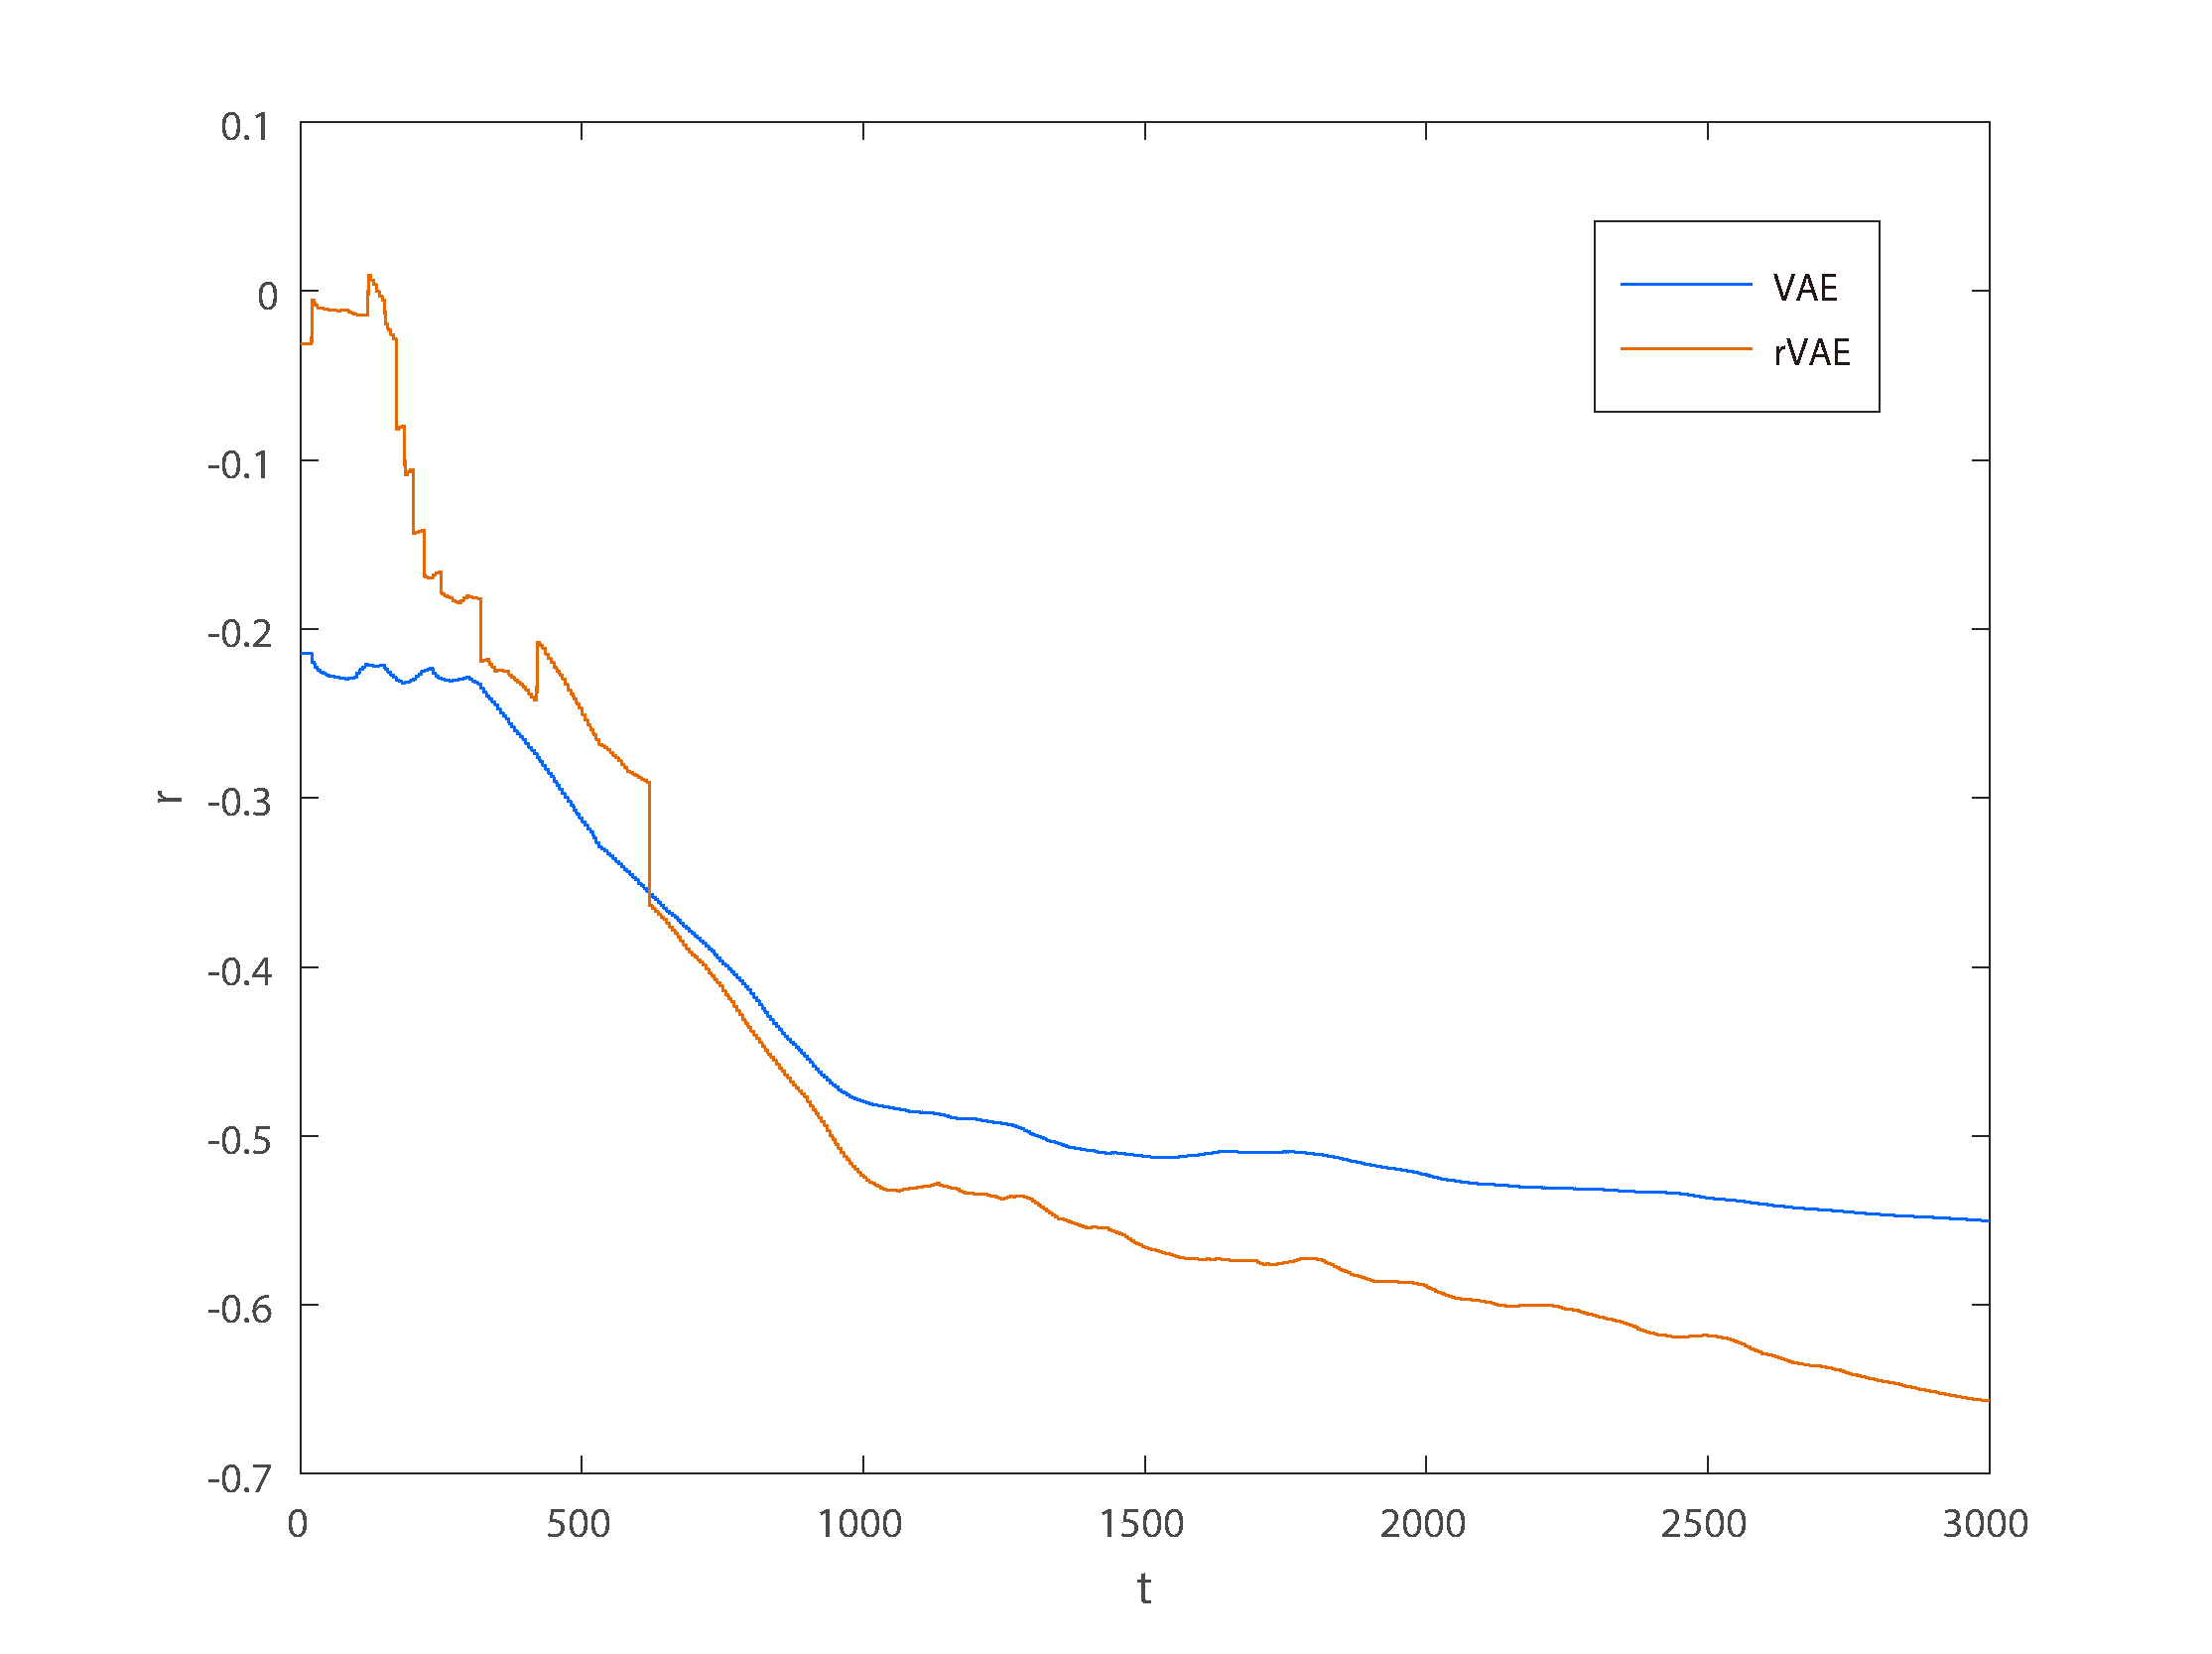
\includegraphics [width=0.85\columnwidth]{fig/fig_corr_t.pdf}
  \bicaption[fig:corr-t]{rVAE和VAE与美感的相关系数随时间的变化}{两种视觉注意熵和美感评分的相关系数随时间的变化曲线。熵的显著性随时间愈发加强。1000ms开始rVAE的曲线稳定保持在VAE曲线的下方。依照发展的趋势,如果继续延长实验时间至超过3000ms,熵的表现可能更佳。}{Fig}{ The correlations between the entropies and the aesthetic scores become more and more significant over time. It is clear that rVAEs consistently sit below the VAEs after 1000 ms. The tendencies show that both curves, especially the rVAEs, could perform better, if the duration were longer than 3000 ms.}
\end{figure}

图\ref{fig:with-user}展现了熵与美感评分的相关性随着被纳入计算的被试人数的增长而逐渐趋于稳定的趋势。图中的曲线结果是通过每次纳入一名随机被试的眼动数据获得的。似乎更多的被试人数会获得更好的与美感评分的关联性,但同时也以为着更高的时间成本和实验开销。

\begin{figure}[H]
  \centering
  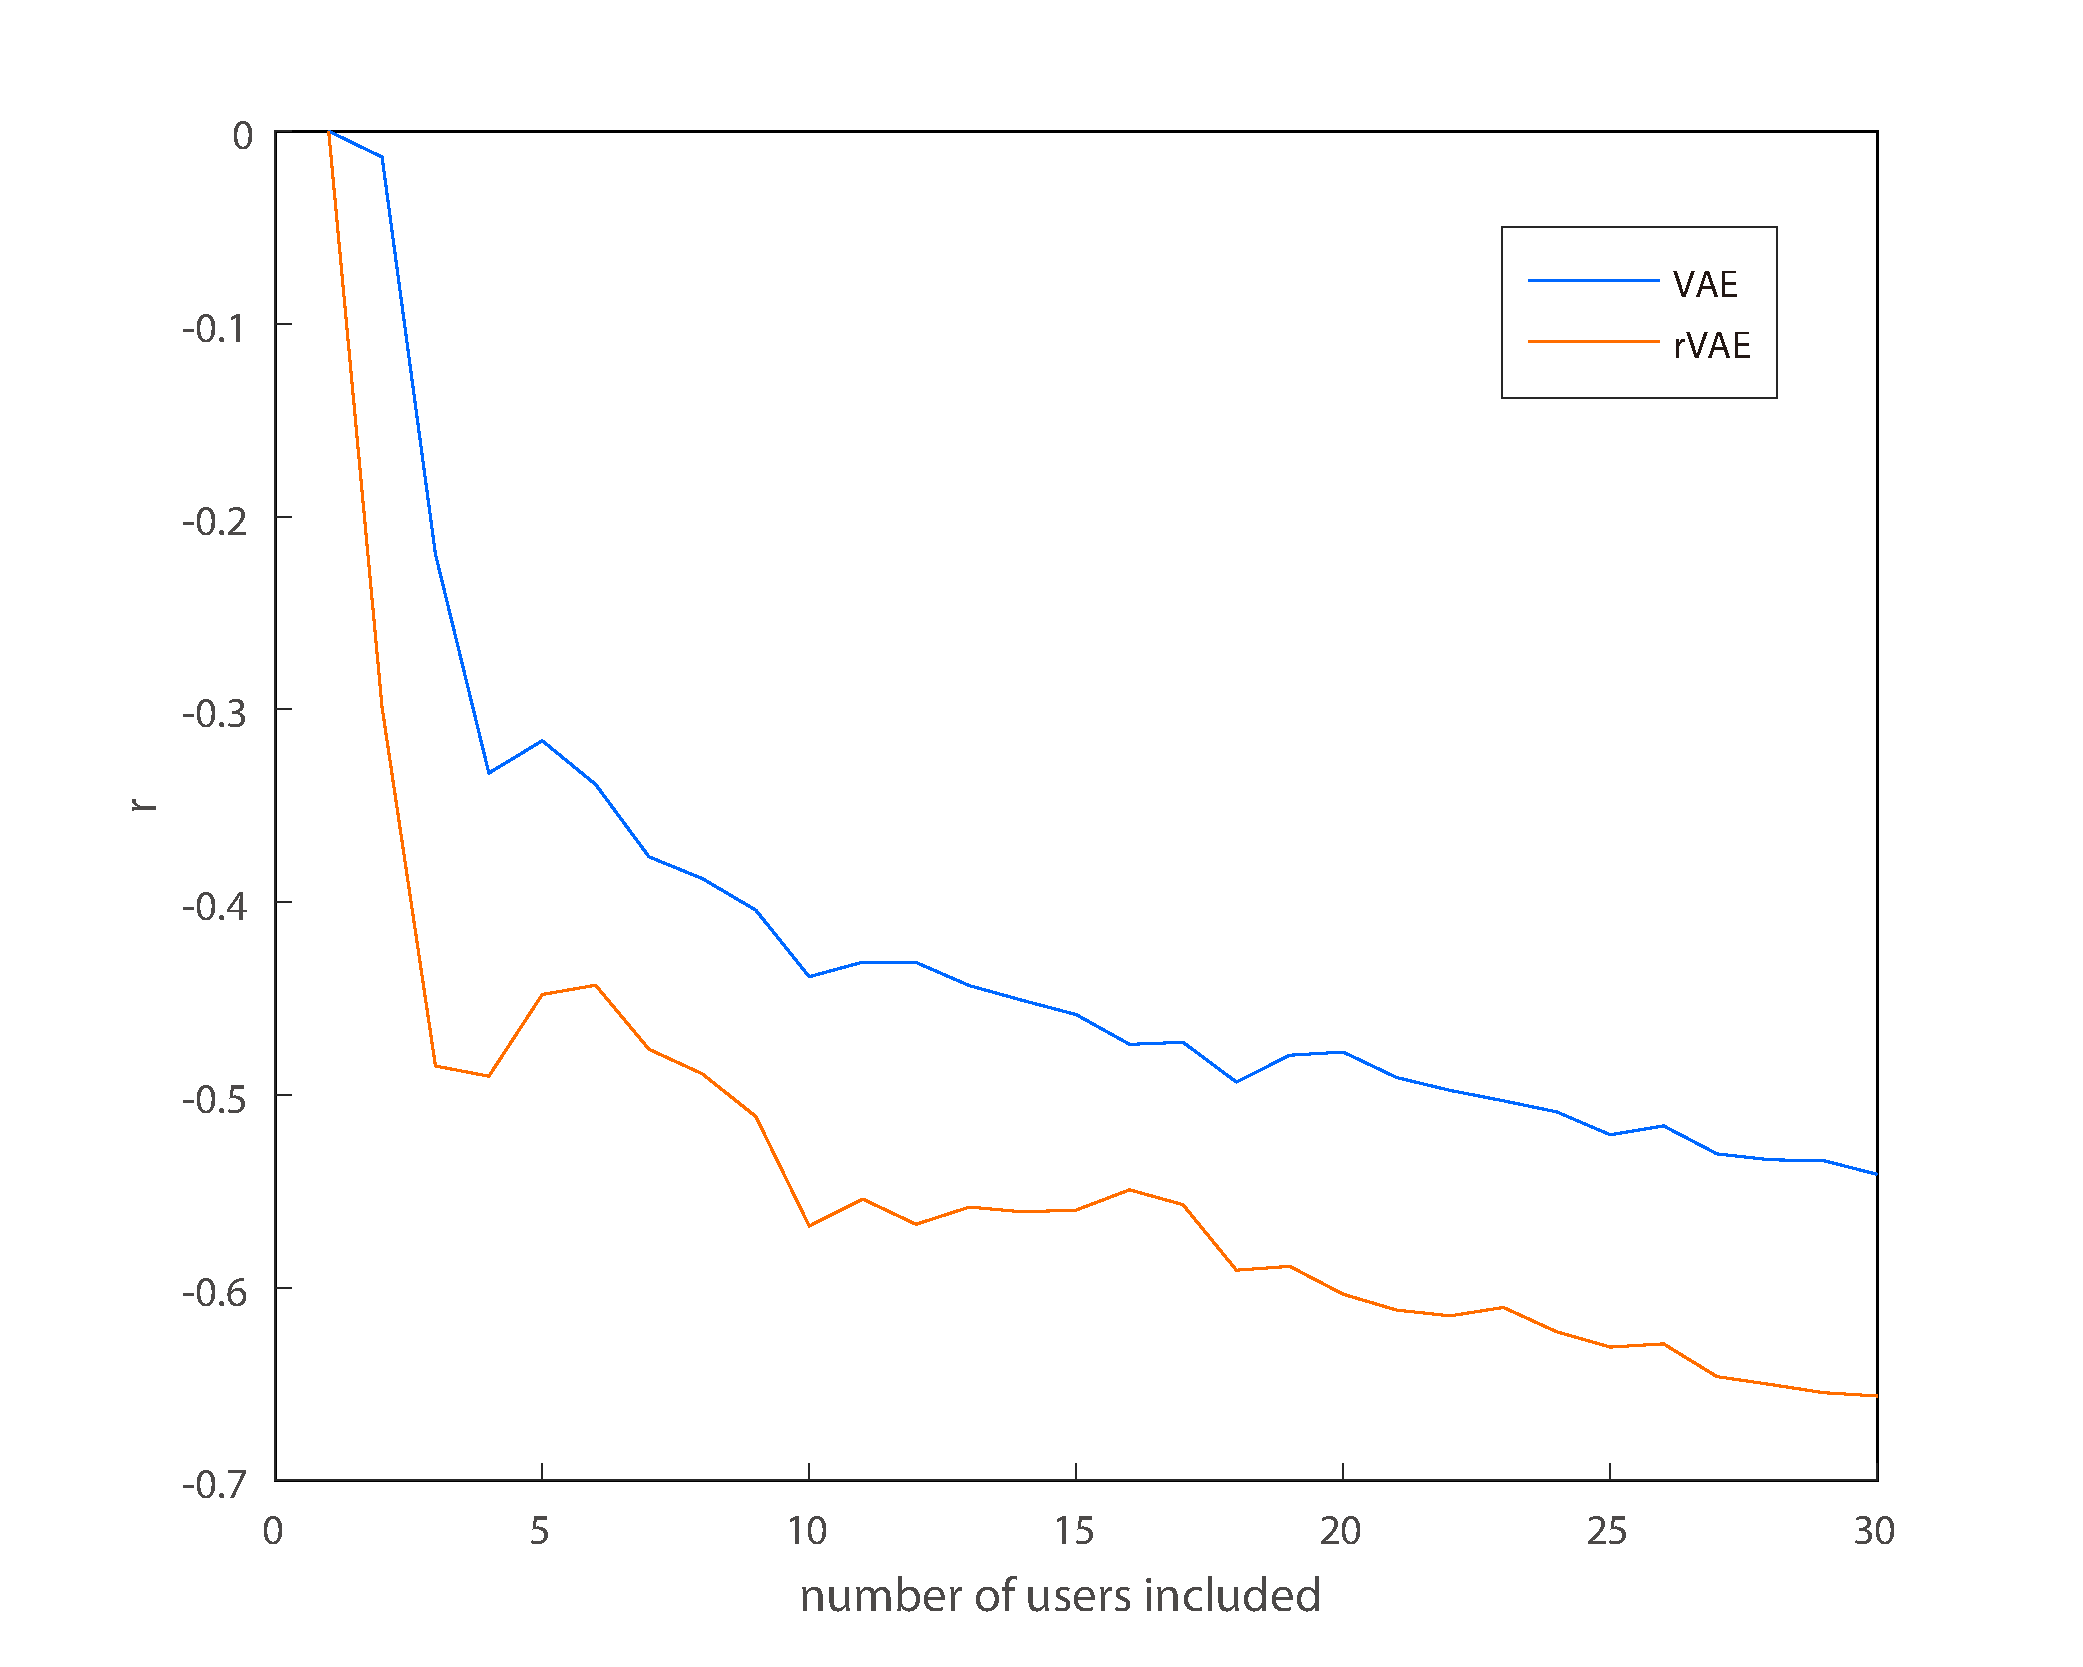
\includegraphics [width=0.85\columnwidth]{fig/fig_user.pdf}
  %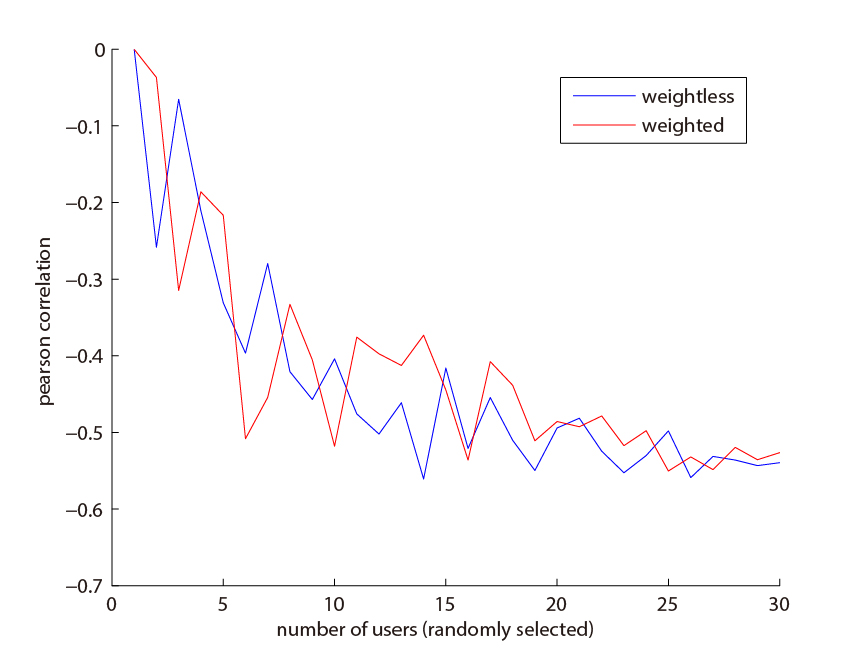
\includegraphics [width=80mm]{fig_vae_user.jpg}
  \bicaption[fig:with-user]{VAE和rVAE关于参与计算的用户人的变化}{VAE和rVAE随参与计算的用户人数的增多逐渐趋于稳定和显著。更多的实验人数(超过30人)可能表现出更好的结果}{Fig}{the correlations between the entropies and the aesthetic scores become more significant with the increasing numbers of subjects. The performance could be better if the number of subjects were larger than 30.}
\end{figure}

到目前为止我们的所有关于熵的计算都是基于热图高斯核$\sigma = 30$的基础上进行的。那么熵与美感的相关性对$\sigma$变化的敏感度如何呢?
\ref{fig:with-sigma}展现了相关系数随高斯核的平滑变化。在相当大的一个$\sigma$取值区间内,VAE和rVAE的表现都很稳定。VAE在$13px-60px$的区间内都有低于-0.5的与美感评分的相关系数;rVAE在$10px-120px$的区间内都有低于-0.6的与美感的相关系数。故熵的表现对于$\sigma$的取值是不敏感的。

\begin{figure}[H]
  \centering
  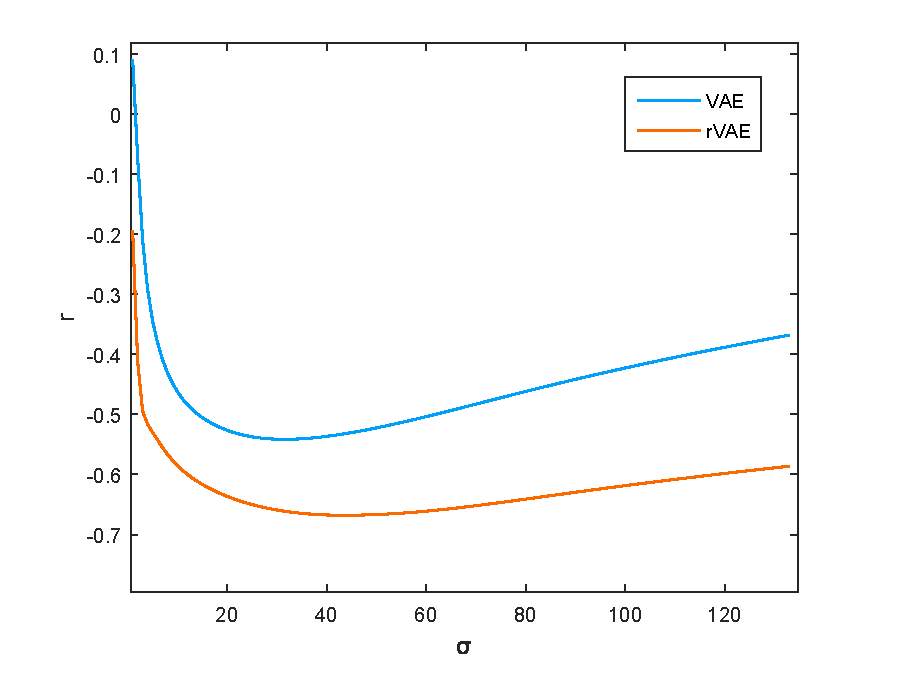
\includegraphics [width=0.85\columnwidth]{fig/fig_sigma.pdf}
  \bicaption[fig:with-sigma]{VAE和rVAE关于高斯核的标准差$\sigma$的变化}{两种视觉注意熵与美感的相关性随热图高斯核标准差的变化的曲线图。曲线较为平滑,在很长一段区间内都保持在各自的极值附近:对VAE,从$20px$到$60px$都保持在-0.5以下,对rVAE,从$10px$到$120px$都保持在-0.6以下并在$40px$左右取得其极值。}{Fig}{The correlations smoothly change with the value of $\sigma$. The performances of both VAE and rVAE are stably approaching their maxima in a rather wide range of the $\sigma$. For VAE, from $20px$ to $60px$, the correlation coefficient stays below -0.5. For rVAE, from 10px to 120px, the correlation coefficient stays below -0.6 and the curve reaches its extremum at about $40px$.}
\end{figure}

上述的分析证实了VAE和rVAE在对美感的推测力方面的稳定性。并且看来,通过加长实验时间、扩大被试的规模和选择合适的$\sigma$取值,它们的表现还可以更好。

\section{讨论与小结}
实验证实了人的美感判断与眼动行为的确存在着联系。对注视序列和热图两个维度的香农熵的探索尝试表明,基于热图的视觉注意熵VAE对美感具有一定的推测里而基于马尔科夫假设的注视序列的熵则没有。VAE,视觉注意熵,可以解释成在分配有限的注意力资源时的混乱度。而他的改进版指标,rVAE,相对视觉注意熵,与我们的感知的美感有显著的相关性($r = -0.65$)。仅仅这单个指标对页面的美感好坏就有相当程度的预测力。

VAE的成功的一部分因素归功于通过高斯核进行的插值,认为眼动注视的分布是连续的。同时3秒内的所有注视都投影在单个平面上,令数据密度更高。而注视序列熵失败的也许可以归咎于其基于时间的统计方式导致的数据量的稀疏。此刻仍很难说它与人的美感判断是无关的。也许未来可以找到更适用的模型来解决这个问题。

一个较低的VAE可以解释人们在眼睛动向和搜索上更少的代价付出。实验中好的网页拥有更小的VAE的趋势支持了流畅理论【】的说法,并一定程度上解释了为什么“好看的就是好用的”【】。VAE是基于眼动注视中的特定信息的。作为一个新的客观的眼动数据量化指标,它显然不仅仅是美感的一种度量,自然中的VAE与我们的观察和驾驶能力更相关。视觉注视在功能性上与鼠标指向很相似,这在一定程度上解释了为什么一些视觉引导相关的设计原则与Fitts规则(选择层级代价经验公式)很相似。

rVAE可以被理解成在屏幕范围的限制下用尽可能小的视觉注意代价(即VAE)去获取尽可能多的信息量(即bVAE)。这与基于进化论美学的“最大效益最小手段”的美学原则是一致的。进化论美学认为人类是为了提高生存和繁衍的成功率而进化出基础审美能力的。

眼动代表了显性和隐形注意的一种合作。虽然我们发现通过眼动行为来预测一个页面的美感至少需要约1000ms的眼动数据,我们对页面的第一印象的产生却只需要50-500ms【】。事实上,50ms仅仅足够完成一个对页面的快速“截屏”,我们的眼睛仍然停留在原地不动。这表明大脑可以通过50ms曝光的残留印象形成的隐形注意热图就作出美感的评价。

\chapter{实验二:图像特征提取}
\label{chap:exp2}

\section{实验目的}
图像特征提取实验的研究对象是审美的客体,在本文中即是网页。通过大量的网页截图样本及其评分,需要论证以下进化论美学在版式特征上的推论:

\begin{enumerate}
  \item 页面版式的视觉复杂度与显著性分布对页面的美感具有推测力
  \item 美感评价较高的页面版式应该具有适中范围的视觉复杂度和适度不平衡的视觉显著分布。
\end{enumerate}

\section{样本与数据}
\subsection{实验样本}
相比于眼动实验受制于实验开销而导致的样本量较小,图像特征提取实验中我们收集了较大规模的网页样本和评分以作为特征提取和机器学习的数据。类似眼动实验的样本来源,初始参与实验的1500张网页页面来自于若干个评选最佳网页设计和最烂网页设计的网站,以及Alexa2017年访问数排名前500名的网站首页。相比于眼动实验,这些页面没有那么具有对好坏的页面设计的代表性,但保证了足够的网页美感差异。通过对熟悉的人脸和图标的筛除,最终留下1447张无重复的页面作为实验样本网页。

所有的样本网页都以且仅以截图的格式参与特征提取实验,没有任何非图像特征如DOM特征,CSS特征等被纳入。这样可以确保特征提取过程的输入信息与人眼浏览这些网页时的输入信息完全一致。

为了确保网页的渲染效果和渲染一致性,浏览器采用现今最主流的浏览器之一的Google Chrome浏览器(版本号57)。屏幕的分辨率被调整至当下主流的全高清($1920\times1280px$)。对于每张实验页面,在确保其加载之后完成后使用Chrome的全屏模式对页面最顶端的部分进行截屏。为了控制变量,仅仅讨论网页的版式信息,截图被去色并重采样成$1280\times720px$的灰度的PNG格式供后续的评分和特征提取。

\subsection{评分系统及过程}
评分采用线上评分的方式,通过在服务器上搭建评分网站实现一定程度上的众包评分。每一个登陆网站参与评分的志愿者需要首先注册一个用户名一边在此后用于跟踪他的评分进度。用户名要求长度至少8个字符,只能包含数字与英文字母。

注册后会显示包含实验说明的页面。具体说明内容见附录\ref{chap:app-survey}。阅读说明后志愿者可以选择再次修改自己的用户名或是开始评分。

开始评分后,等待评分的页面会全屏显示在志愿者的浏览器上。评分采用二值化,用户通过键盘的“左”、“右”键分别表示“不好”和“好”,并进入下一张的评分。

对于每个评分者,由于样本量较大,不要求完成全部的网页评分,且可以多次登录继续评分。每次评分的网页按随机顺序出现,但不会重复。

对于每个被评分的页面,后台系统会自动平衡其曝光的几率,使得所有的页面都能得到差不多的评分被评分次数。如果一个页面的前10次评分全部相同,则不再继续参与评分以减少总共需要评分的次数。

\subsection{参与者与结果}
截止至机器模型训练开始,共有55人参与了评分,评分人群的背景方差较大,年龄分布在20岁到50岁之间,大部分参与者为中国籍交大学生,也有部分外国籍交大学生和中国籍非交大师生参与。评分共累计29310次。全部1447个样本页面中,138个页面获得10次一致的评分,868个页面获得21次评分,441个页面获得22次评分。

给一次“不好”的评分记0分,给一次好的评分记1分,通过计算每个页面的平均值可以得到其美感的好评率,我们以此作为后续试验的美感评分。所有1447张页面的美感评分的频率分布直方图如图\ref{fig:exp2_score}。

\begin{figure}[H]
  \centering
  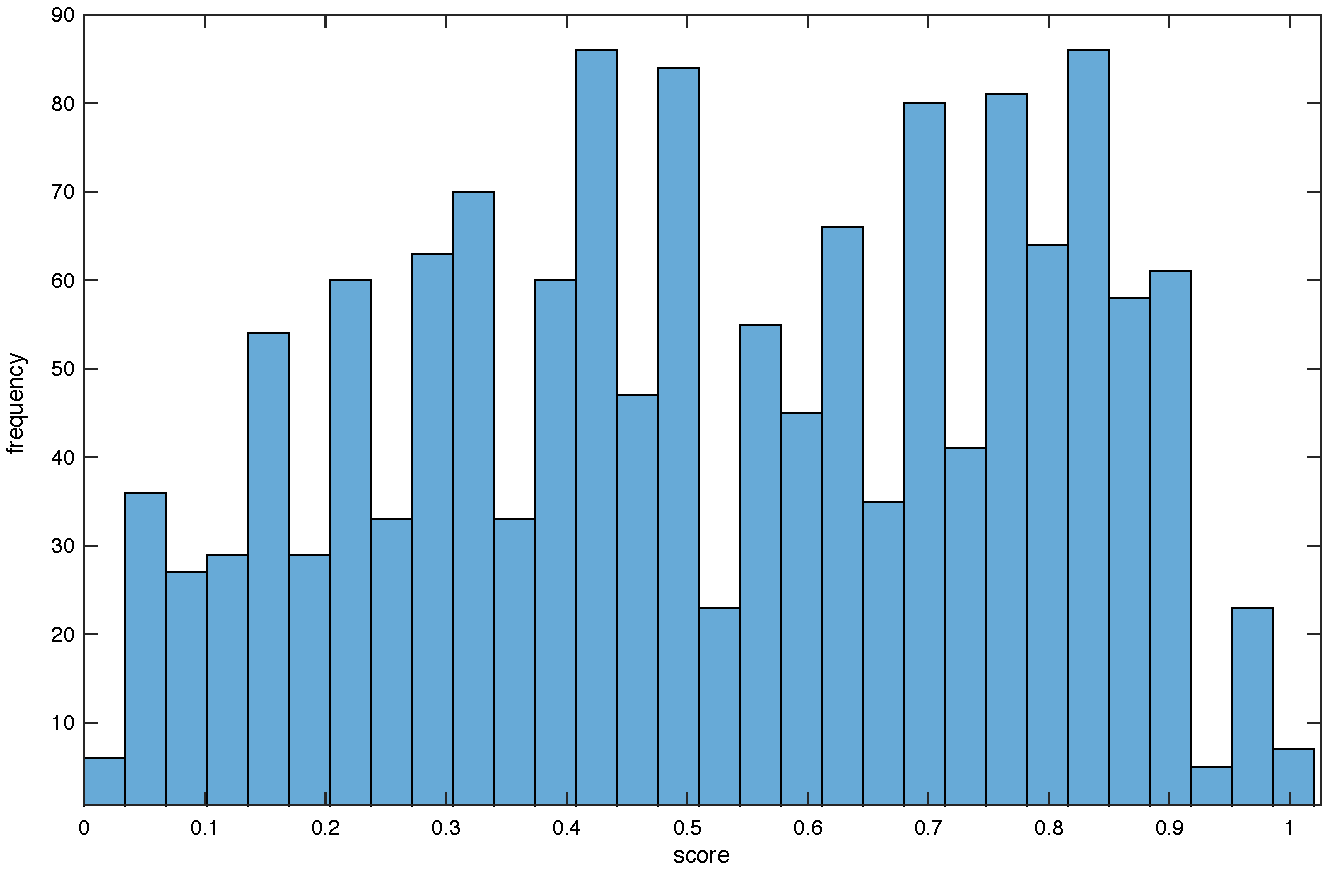
\includegraphics[width=0.75\columnwidth]{fig/fig_exp2_scores.pdf}
  \bicaption[fig:exp2_score]{特征提取实验的网页得分的频率分布直方图}{特征提取实验的网页得分的频率分布直方图}{Fig}{The histogram of the scores of the 1447 webpages}
\end{figure}

\section{特征提取与分析}
\subsection{验证方法}
Logistic回归方程\ref{formula:logit}是通过sigmoid函数处理后的多项式回归方程,在分类问题上的应用优于线性回归。我们通过Logistic回归的系数显著性来验证一个特征对于美感评分是否具有推测能力。其显著性代表着在拒绝该特征对美感具有分类能力的概率。

\begin{equation}
  Logit(X) = \frac{1}{1 + e^{-X^{T}\beta}}
  \label{formula:logit}
\end{equation}

其中$\beta$为参数,$X$为增广的数据向量

基于视觉复杂度和视觉重点分布对美感具有推测力的假设,下面一共挖掘并提取了4类特征。分别是网格复杂度、信息密度分布、空白分布与显著性分布。这些特征中没有纯粹代表复杂度或是重点分布的特征,如同实验一讨论的VAE一样,它们一般都同时包含了两方面的信息。

\subsection{网格复杂度}
网格复杂度描述页面元素之间的对齐和比例情况,是一种版式复杂度,同时与元素边界的位置分布也有关。

对齐指的是并列元素的边界之间的是否相互共线;比例指的是并列元素在对齐方向上的长度比值是否简单。在同样的内容元素的前提下,对齐较严格、比例较简单的页面布局具有较低的视觉复杂度可以降低视觉负担,反之则具有较高的视觉认知负担。

Kohlschutter et al. 2008 提出了对页面的横纵坐标上的像素的灰度值累加到一维向量的方式来考量垂直和平行方向上的对齐情况\citen{Kohlschutter2008},并由此获得一个1280维的向量和一个720维的向量。对于出现明显对齐边界的地方,一维向量会表现出明显的高峰或是凹陷。\ref{fig:grid}示例了如何通过堆积算法提取网格信息。具体的特征提取过程和如下:
\begin{enumerate}
  \item 使用canny算法提取页面上的轮廓线(等高线Contour)
  \item 对轮廓线图片进行垂直累加和横向累加,分别得到一维向量H和V
  \item 对H和V计算差分,即相对于像素的梯度【公式】,得到dH和dV
  \item 对dH和dV进行噪声滤除,只保留绝对值大于给定的阈值T的的维度,其余维度归零。由于一条边界两侧的梯度总是表现出一正一负的特性,再对结果去除负值,只保留正边界的差分
  \item 通过计算得到的dH和dV得到每两两边界之间的距离,构成一纵一横两个网格距离向量。
\end{enumerate}

\begin{figure}[H]
  \centering
  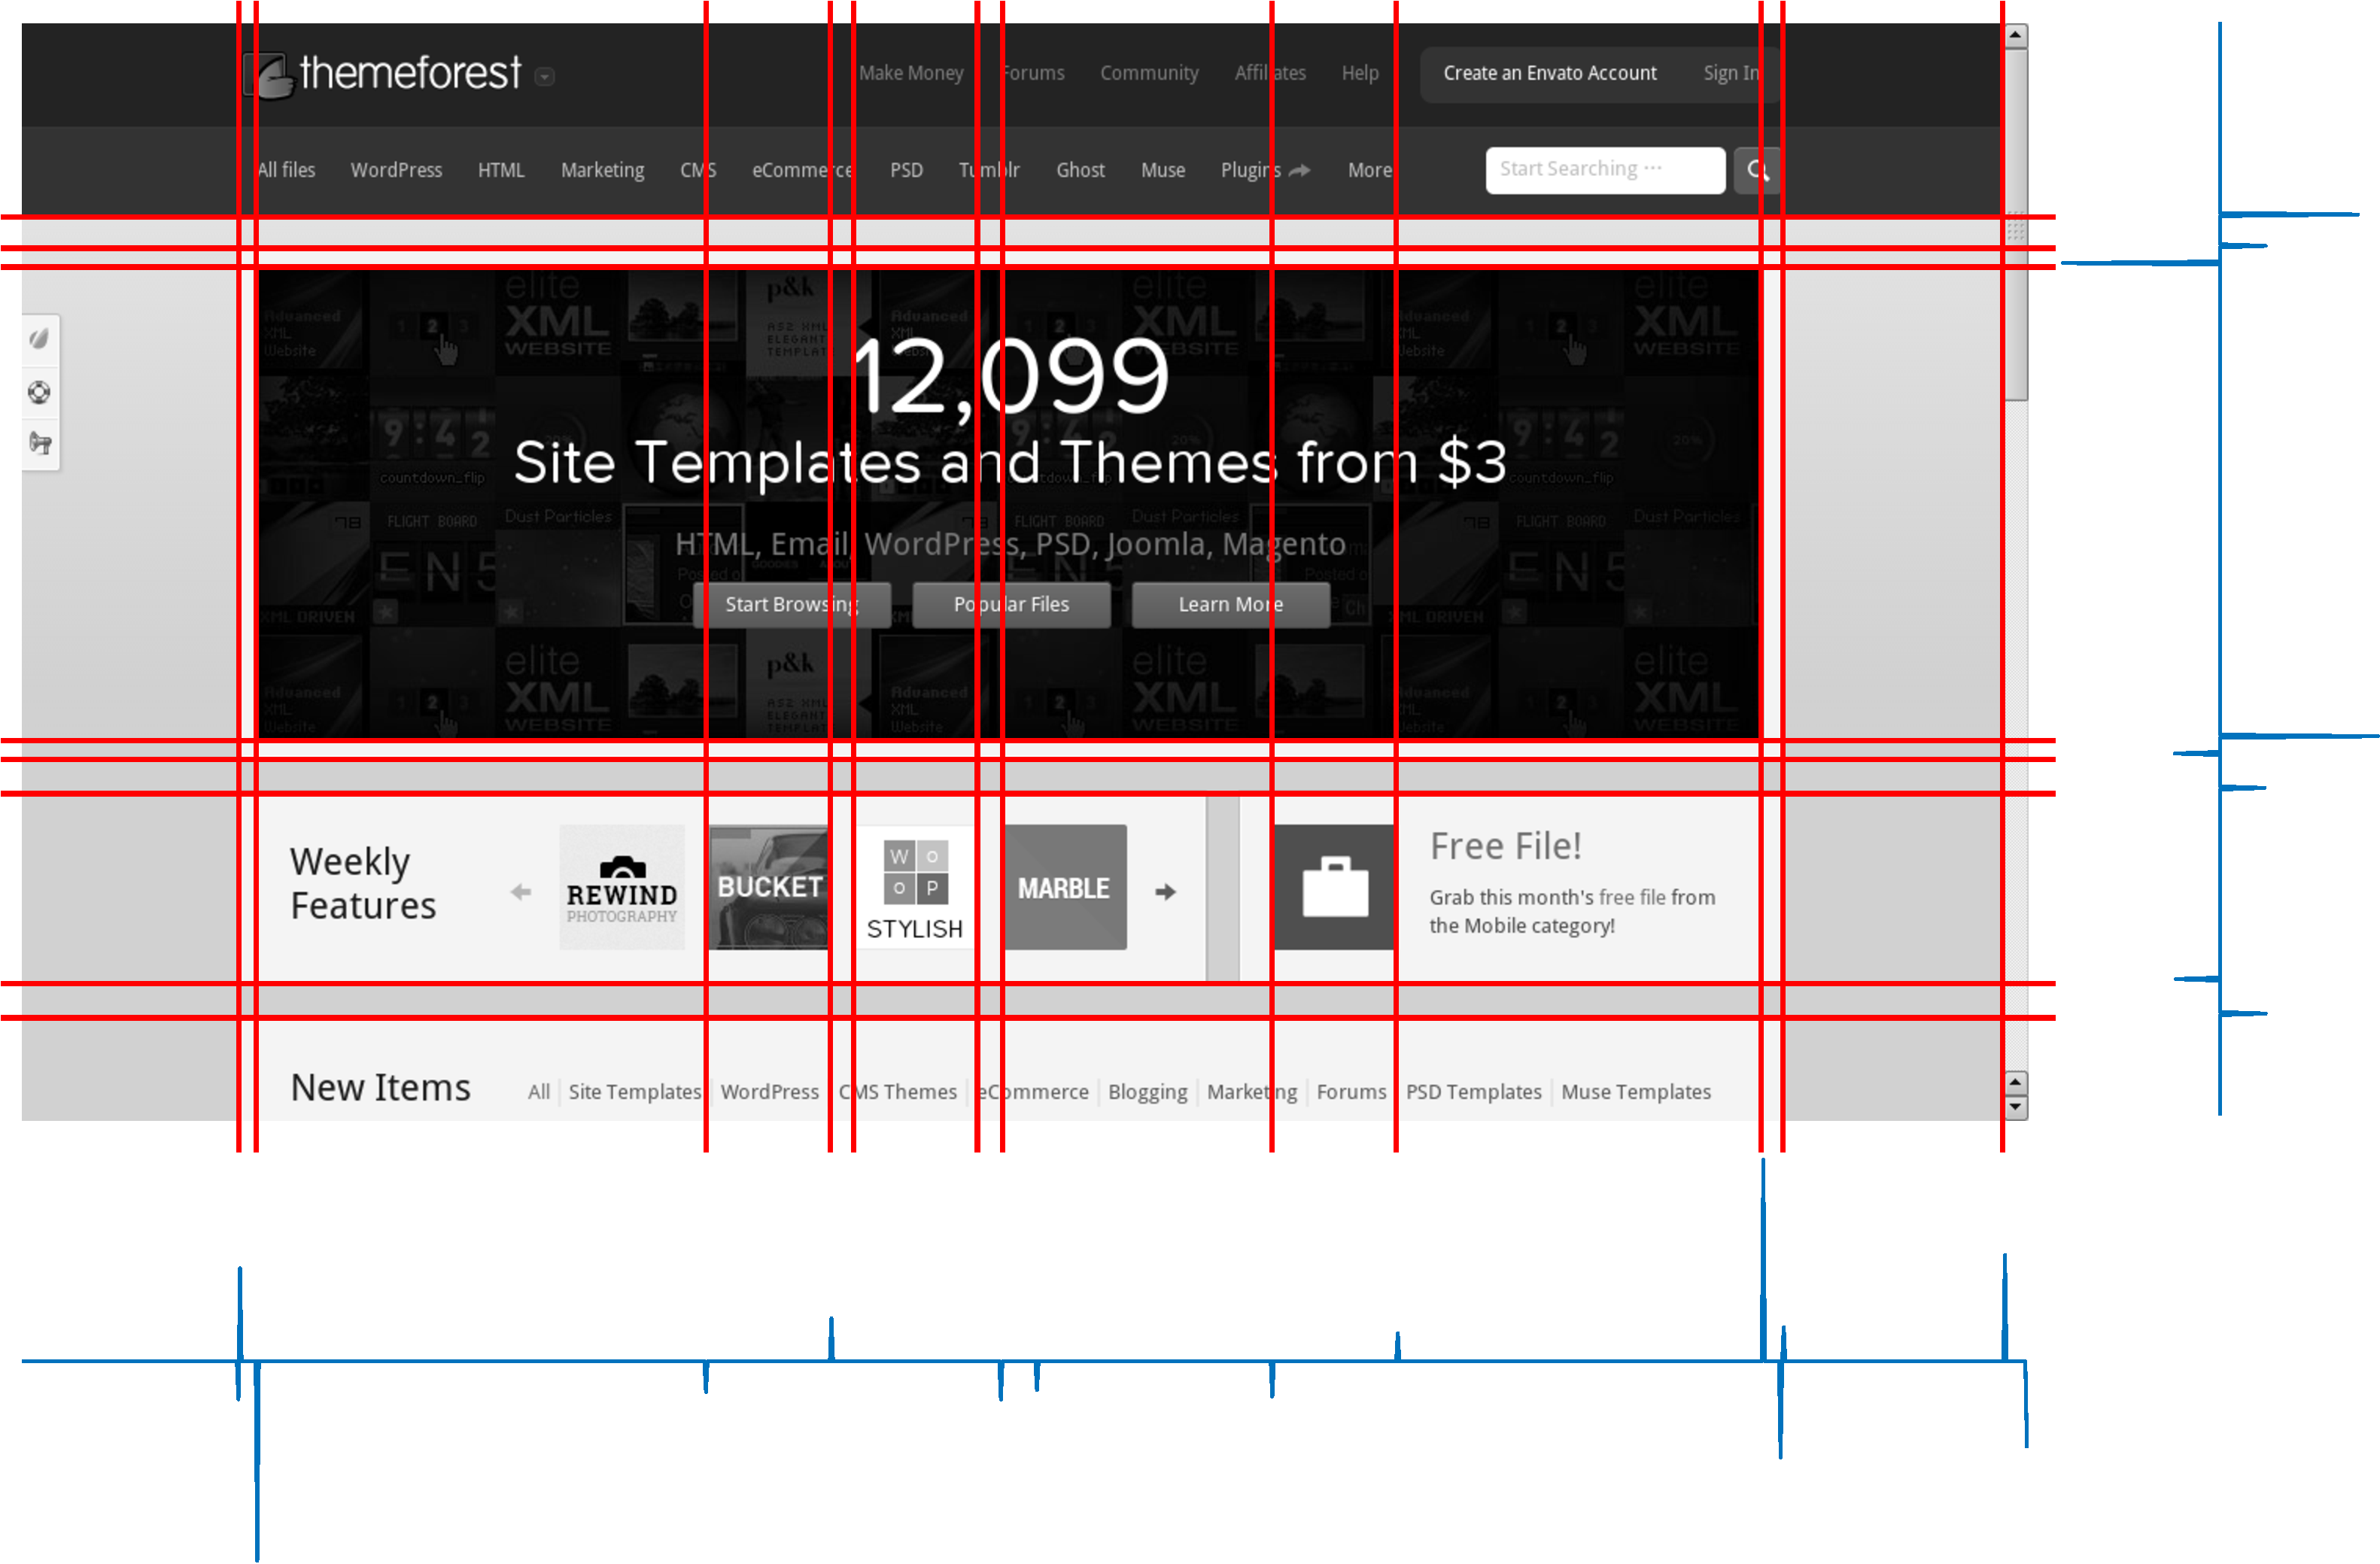
\includegraphics[width=0.85\columnwidth]{fig/fig_grid.pdf}
  \bicaption[fig:grid]{网格复杂度特征提取示意图}{网格复杂度特征提取示意图,纵横的蓝色曲线分别为一维向量V和H,在此基础上可以对画面分割得到网格(红色曲线)。}{Fig}{an example of the calculation of grid complexity feature, the blue curves are the mono vectors V and H, the red lines are the grids generated from the vectors.}
\end{figure}

对上述步骤4中得到的差分向量和步骤5中得到的网格距离向量,通过基本的统计归纳获得一系列的特征。这些特征的名称、计算方式和Logistic回归验证的显著性在表\ref{tab:grid}中列出。

\begin{table}[H]
  \centering
  \small
  \begin{tabular}{lllrr}
    \hline
     特征名称 & 计算方式 & 回归系数 & Prob$>$F \\
    \hline
    纵向网格数量 & 统计纵向网格数量 & -4.36 & $9.8e^{-10}$\\
    横向网格数量 & 统计横向网格数量 & 1.32 & 0.12\\ %
    纵向均衡性方差 & 对纵向网格按$S = \frac{1}{\sum | X_i - X_{n-1}|}$计算均匀性,统计方差 & -1.6 & $4.3e^{-03}$\\
    横向均衡性方差 & 同上对横向网格计算 & -6.42 & 0.10\\
    纵向均衡性均值 & 同方差方法对均匀性计算均值 & -1.87 & 0.065\\
    横向均衡性均值 & 同上对横向网格计算 & 11.72 & 0.10\\
    \hline
  \end{tabular}
  \bicaption[tab:grid]{网格复杂度特征的显著性}{网格复杂度特征的显著性}{Table}{The significance of grid complexity features}
\end{table}

\clearpage
网格复杂度的推测力与其他图像特征相比不算很显著。但其纵向网格数量和纵向均衡性方差分别都对美感表现出了显著的负相关推测力。一方面这表明网页的行向排版(通过纵向特征统计)比列向排版(通过横向特征统计)对美感更有推测力;另一方面表明美感评分好的网页往往具有更均衡而有序的网格排版。

\subsection{占空分布}
\begin{figure}[H]
  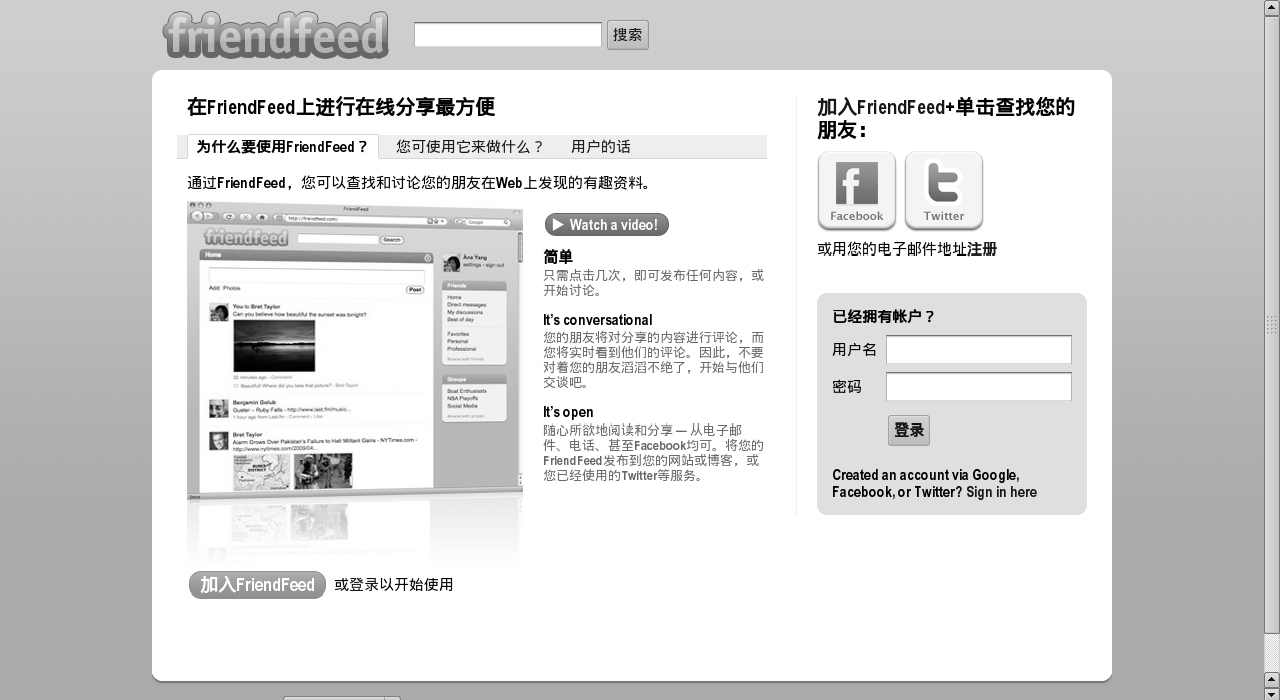
\includegraphics[width=0.5\columnwidth]{fig/fig_exp2_eg.jpg}
  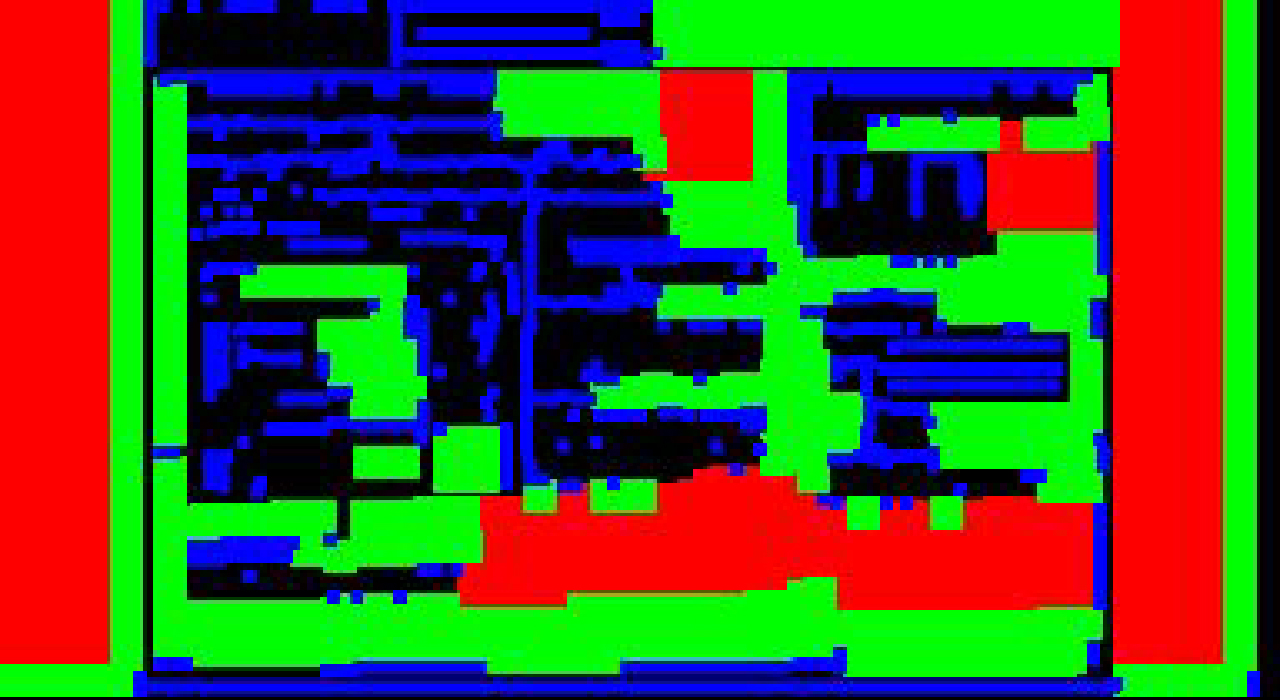
\includegraphics[width=0.5\columnwidth]{fig/fig_blank.jpg}
  \bicaption[fig:blank]{占空分布的示意图}{网页例图(左)和对应的占空分布的计算过程(右),红绿蓝分别代表大中小的“画笔”所填充的空白空间}{Fig}{an example of the calculation of the blank distribution where red-, green-, blue-colored areas respectively represents the areas filled by big, medium and small 'paint pens'.}
\end{figure}

占空分布统计信息复杂度为零的区域的分布情况。依次采用大($100\times100$)、中($30\times30$)、小($10\times10$)三种画笔对画面的空白区域进行填充(一旦被先前的画笔填充就不能再填充),得到三种画笔各自的填充的联通块的数量、面积、最值和方差。图\ref{fig:blank}显示了一张网页例图(左)和占空分布的计算过程(右),红绿蓝分别代表大中小的“画笔”所填充的空白空间。这些特征的名称、计算方式和Logistic回归验证的显著性在表\ref{tab:blank}中列出。

\begin{table}[H]
  \centering
  \small
  \begin{tabular}{lllrr}
    \hline
     特征名称 & 计算方式 & 回归系数 & Prob$>$F \\
    \hline
    $100\times100$空白面积 & $100\times100$的“方块画笔”填充的空白区域面积 & 10.29 & $1.9e^{-05}$\\
    $30\times30$空白面积 & $30\times30$的“方块画笔”填充的空白区域面积 & 6.81 & $2.7e^{-10}$\\
    $10\times10$空白面积 & $10\times10$的“方块画笔”填充的空白区域面积 & -5.61 & $9.6e^{-04}$\\
    \hline
  \end{tabular}
  \bicaption[tab:blank]{占空分布特征的显著性}{占空分布特征的显著性}{Table}{The significance of margin distribution features}
\end{table}

\clearpage
使用方块画笔对空白进行填充的方式相比直接计算空白的面积更好地提取了横平竖直的视觉坐标下,页面上占空分布的情况。

表\ref{tab:blank}的结果表明,“大中小”三种占空的面积对美感都有显著的推测能力。“大”和“中”表现出正相关,“小”表现出负相关。这意味着在不同内容区块之间留白较大而在同类区块之间留白较小的情况下,网页页面版式更有可能取得较高的评价得分。这与类间间距越大,类内间距越小则越美观的观点是一致的,其实代表着一种信息的有序性。

\subsection{信息密度分布}
\begin{figure}[H]
  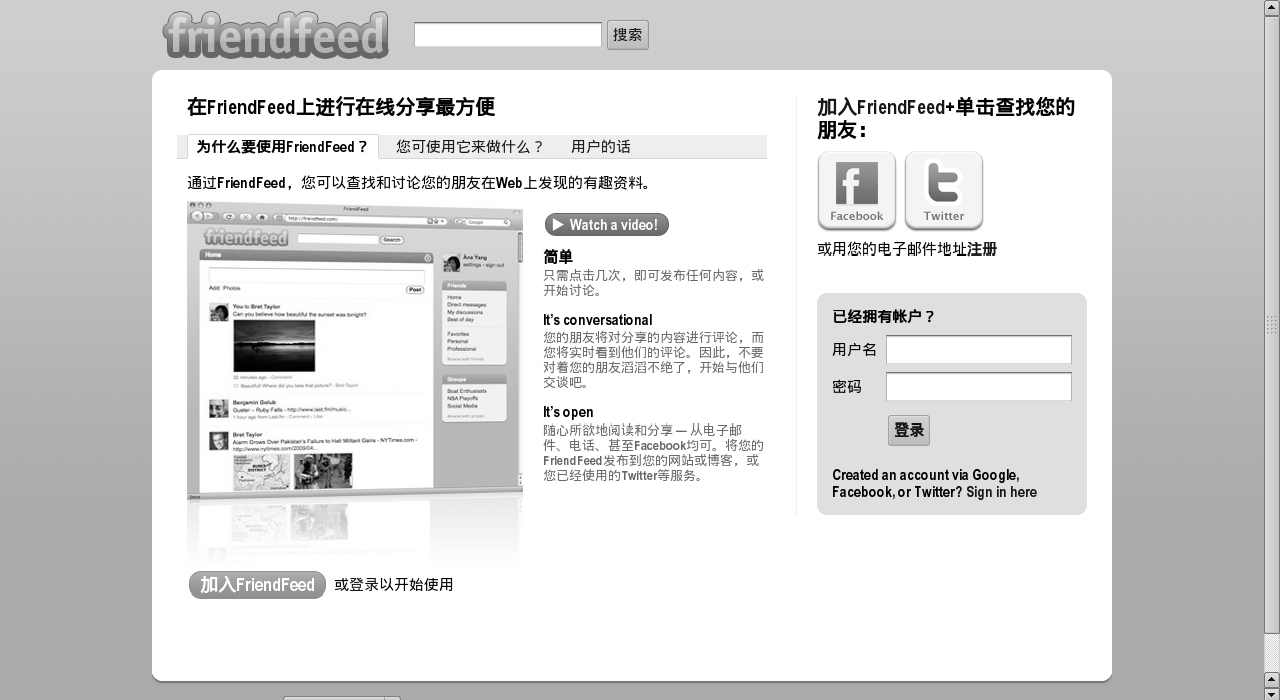
\includegraphics[width=0.5\columnwidth]{fig/fig_exp2_eg.jpg}
  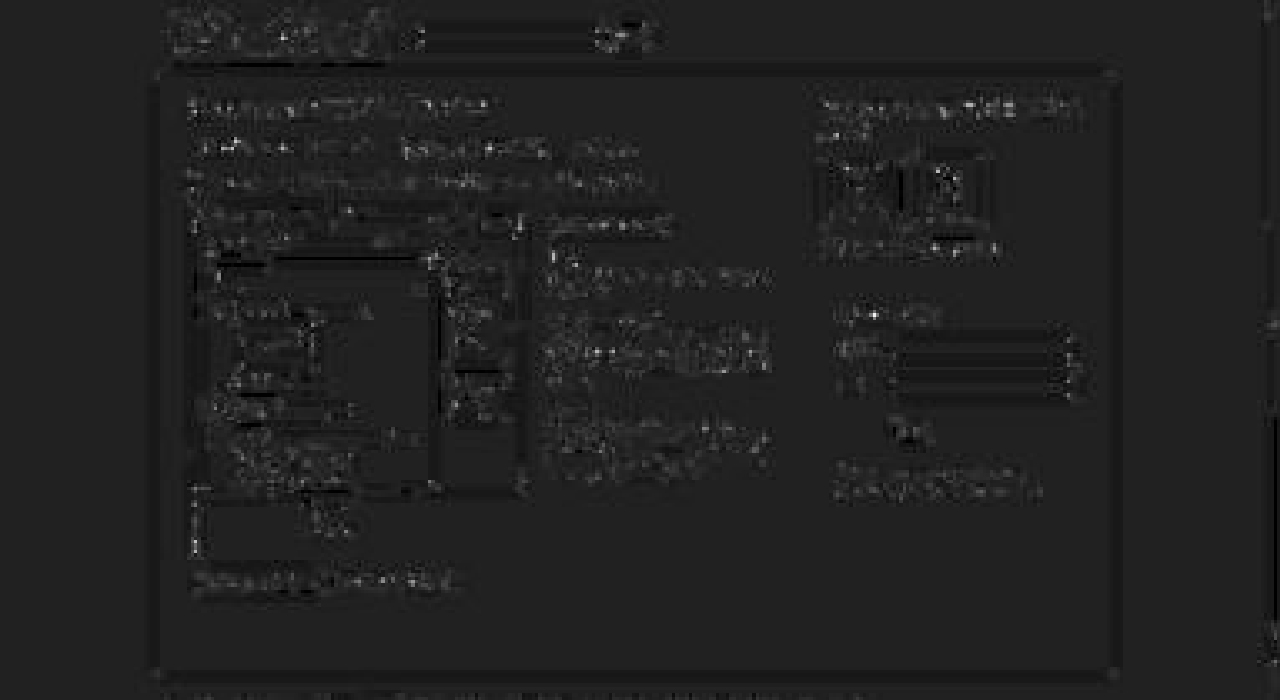
\includegraphics[width=0.5\columnwidth]{fig/fig_info.jpg}
  \bicaption[fig:info]{信息密度分布的示意图}{网页例图(左)和对应的信息密度分布的计(右),白点代表被认为是信息高密度的拐点}{Fig}{an example of the calculation of the information density distribution. The white dots are where information is considered to be dense.}
\end{figure}

信息密度分布从空白分布相反的角度考量页面上信息分布的疏密。通过统计可能是信息高密度的边沿拐点在页面上的分布来考量信息密度的分布。具体计算中将页面分块成3行乘4列的12块区块,得到由每一个区块中的拐点个数构成的12维向量。对此向量统计其最值、均值、方差作为特征。这些特征的名称、计算方式和Logistic回归验证的显著性在表\ref{tab:density}中列出。

\begin{table}[H]
  \centering
  \small
  \begin{tabular}{lllrr}
    \hline
     特征名称 & 计算方式 & 回归系数 & Prob$>$F \\
    \hline
    $(0, 0)$处信息量 & 统计0行0列网格内的拐点数量 & 2.03 & $0.067$\\
    $(0, 1)$处信息量 & 同上 & 3.16 & $4.9e^{-06}$\\
    $(1, 0)$处信息量 & 同上 & 2.79 & $1.2e^{-03}$\\
    $(1, 1)$处信息量 & 同上 & 2.79 & $1.9e^{-03}$\\
    $(2, 0)$处信息量 & 同上 & 2.19 & $0.035$\\
    信息密度最大值 & 统计各区块拐点个数的最值 & -0.58 & $0.083$\\
    信息密度方差 & 统计各区块拐点个数的方差 & -1.77 & $8.4e^{-05}$\\
    信息密度均值 & 所有区块拐点个数的均值 & -29.12 & $1.3e^{-04}$\\
    信息密度重心 & 统计整体拐点重心的横坐标 & 19.81 & $3.8e^{-04}$\\
    \hline
  \end{tabular}
  \bicaption[tab:density]{信息密度分布特征的显著性}{信息密度分布特征的显著性}{Table}{The significance of information density distribution features}
\end{table}

结果表明总体而言信息密度相关的特征与美感评分有显著的相关性。局部上,画面上特定位置区域的局部信息量对美感评分的推测力尤为显著,意味着人们在眼动习惯上虽然有着各自不同的习惯,但是对画面上特定位置(左上,中部,左侧)都表现出了较为一致的优先关注和判断。这可能与现代人的文字阅读习惯有关,也许在具有不同阅读方向习惯的文化环境(如阿拉伯)中,这些影响美感评价的关注点会有所不同。

\subsection{视觉显著性分布}
视觉显著性是对眼动的视觉注视点的分布的一种模拟,是一种视觉重点分布为主的特征。采用Itti et al. 2005中对视觉显著性的算法\citen{Itti2005},用基于高速金字塔的明度梯度图构建页面的视觉显著性分布。

\begin{figure}[H]
  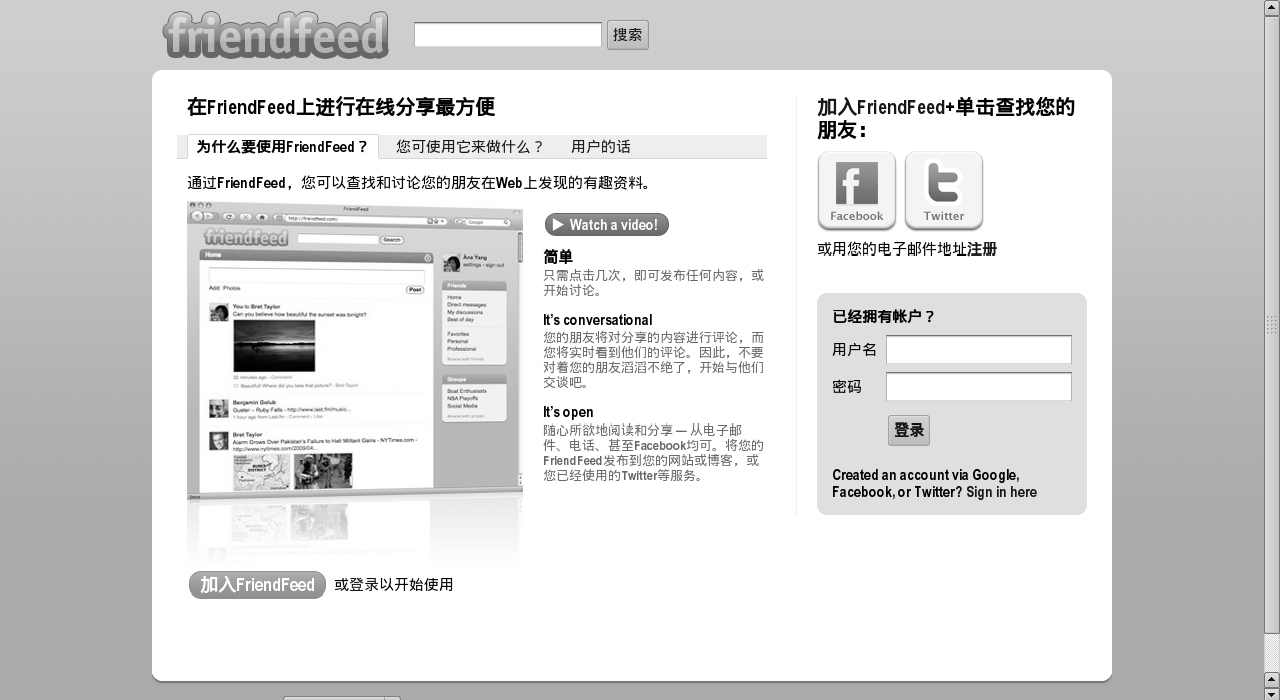
\includegraphics[width=0.5\columnwidth]{fig/fig_exp2_eg.jpg}
  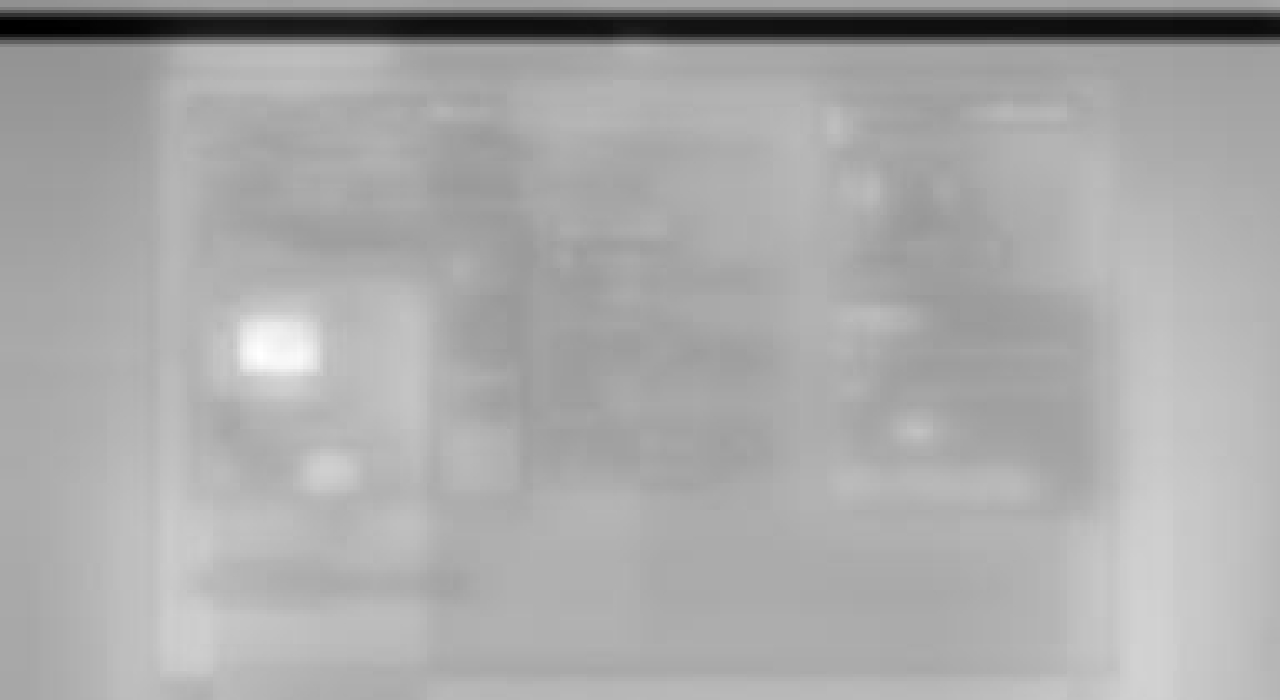
\includegraphics[width=0.5\columnwidth]{fig/fig_saliency.jpg}
  \bicaption[fig:info]{视觉显著性分布的示意图}{网页例图(左)和对应的视觉显著性分布的计(右),明度代表该区域的视觉显著性}{Fig}{an example of the calculation of the saliency distribution. The saliency of an area is represented by the luminance}
\end{figure}

相关特征的名称、计算方式和Logistic回归验证的显著性在表\ref{tab:saliency}中列出。

\begin{table}[H]
  \centering
  \small
  \begin{tabular}{lllrr}
    \hline
     特征名称 & 计算方式 & 回归系数 & Prob$>$F \\
    \hline
    显著性方差 & 各区块的显著性方差 & -13.53 & $2.9e^{-11}$\\
    显著性均值 & 各区块的显著性均值 & 17.42 & $1.2e^{-12}$\\
    显著性重心x & 整体显著性的横向重心:$G = \frac{\sum V_i X_i}{\sum V_i}$& 5.98 & $4.2e^{-04}$\\
    显著性重心y & 整体显著性的纵向重心:$G = \frac{\sum V_i Y_i}{\sum V_i}$ & 4.78 & $8.5e^{-10}$\\
    \hline
  \end{tabular}
  \bicaption[tab:saliency]{视觉显著性分布特征的显著性}{视觉显著性分布特征的显著性}{Table}{The significance of saliency distribution features}
\end{table}

视觉显著性相关的特征在四类特征中表现出了最强的美感推测力。结果表明对于每个区块自身而言,区块内部的显著性方差越小,越有可能取得更高的美感评分;而整体而言,显著性重心的适度倾斜对美感评分有积极的贡献。这一定程度上论证了我们队适度视觉复杂量和适度视觉重点分布不平衡的假设。

\section{小结}
通过对1447个页面中的四类特征的提取和Logistic回归的简单验证,表明网页视觉复杂度和视觉重点分布相关的特征对美感具有一定的推测性,并很大程度上论证了第\ref{chap:hypothesis}章中关于视觉复杂度与视觉重点分布的假设。

上述的四类特征的挖掘方法仍存在较大的探索空间:一方面更精准地挖掘到需要的描述的对象如复杂度、显著性、分布的特性,另一方令其对美感表现出更强的推测能力。

\chapter{网页版式评分系统的工程实现}
\label{chap:application}

网页版式评分系统是对人的审美能力的一种有限模仿。通过第\ref{chap:exp2}章中对视觉复杂度和视觉显著性分布的相关特征对美感的推测力的证实,用这些特征训练得到的模型即可以作为版式评分系统的评价内核。这一章对网页版式评分系统的工程实现展开讨论:\ref{sec:app-app}节简述版式评分系统的应用场景;\ref{sec:app-shape}节给出版式评分系统的形态构想;\ref{sec:app-core}节分析系统中的两个核心模块——特征提取和机器学习之间的关系和各自的必要性;\ref{sec:app-tech}节分数据流向和模块化两部分具体阐述系统的架构和技术应用。

\section{应用场景}
\label{sec:app-app}
一个版式设计的好看的页面往往意味着更专业的服务水平、更高的可信度、更好的可用性\cite{Casal2008The, Li2010Increasing, Lindgaard2011}。因而网页版式美感评分系统作为一种审美模拟系统,可以直接应用于需要替人类预先判断网页的版式审美的场景。例如为搜索引擎增添一项依照美感进行排序的功能,替用户先“看一遍”这些搜索结果,并把好看的挑选出来优先呈献给用户。

而另一方面,互联网时代对大规模内容合理呈现的需要使得设计自动化获得广泛的应用场景。这类设计有着庞大的需求规模,紧迫的设计时间,一般的品质要求和紧贴时代的风格要求。对于较为有前景的生成式设计系统而言,一个出色的版式评分系统就是它的眼睛,赋予自动化设计以审美能力。

\section{形态构想}
\label{sec:app-shape}
\subsection{单调服务}
网页版式评分系统在应用中应该以怎样的面目出现?可以确定的是,作为一个对输入给出评分性响应的系统,它本质是一种服务。它应该运作在服务器上,通过对外暴露的应用程序接口(Application Programming Interface, API)实现与客户端的沟通,并根据他们的需求向他们提供服务。

评分系统应包括且仅仅包括与美感评分相关的功能,不掺和任何为迎合个别类型的客户端需求而实现的功能。服务功能上的单调性让系统更纯粹,更独立,更灵活具有移植性,从而有更广阔的应用场景。

\subsection{RESTful API的设计风格}
版式评分系统本质是一种“审美”服务。这种服务有着多样的应用场景,可能接收多种类型的请求,并需要以多种状态返回他的计算结果。

RESTful API的概念由Roy Fielding在2000年提出\cite{Fielding2000}。是英文Representational state transfer的缩写。作为一种应用设计风格,RESTful API需要满足端对端架构、无状态、可缓存、层式系统、在有需求时生成代码和统一接口六条设计原则\cite{Paliulioniene2013, Richardson2008}。其中无状态性是他的核心原则,这要求在客户端与服务端之间的交互在请求之间是无格式形态的,服务端的数据结构不会向客户端暴露,客户端的请求数据也不会直接存储到服务端,双方以各自的形式来管理数据,对需求的数据形态的要求都在请求报表的表头(Header)中包含。

对于网页版式评分系统而言,无论是请求还是响应的资源都是多形式的:需要评分的对象可能是不同格式的图片数据、url列表、单个url,希望系统返回的结果可能是得分列表(包括XML或JSON格式的)、URL对应的截图或是截图列表,亦可能是多种格式的。RESTful API的设计风格让系统在提供服务方面具有更好的适应性和自解释能力,能够被应用在更广的使用场景中。

\subsection{可发展}
如同人的穿搭审美在不停变化,过去时髦的东西再未来可能显得老土。评分系统的审美也应是与时俱进的,而不应纯粹只依照先天审美因素进行美感评判。对于评分环节依赖机器学习实现的系统,这种与时俱进是易于实现的。通过不停地获取新的样本进行一次性的模型更新训练,可以让参数发生随时间的逐步变化,实现与时代审美风格的与时俱进。

\section{核心实现方式}
\label{sec:app-core}
版式评分系统包含了比单纯的特征推测力更广的内容。依照实验二的思路,版式评分系统的核心模块应为分为特征提取和机器学习两部分。而事实上,由于其输入是一张静态的黑白网页截图,其输出是对这张截图的版式美感的评分预测,版式评分系统的本质是一个图像信息处理系统。这很自然地生出一个疑问,即特征提取是否存在必要性,有没有可能单纯通过现今广泛应用在图像识别领域的卷积神经网络等机器学习技术来直接实现网页版式的美感评价?

机器学习指不通过明确编程而让电脑获得学习能力的一类计算机科学\cite{Koza1996},它利用一些源自统计学的数值分析方法,对大量的数据样本进行迭代式的参数收敛,以获得对新的数据样本具有分析能力的数学模型,是近期的热门话题。常见的机器学习模型有较为基础的线性回归、逻辑回归(Logistic regression),进一步的支持向量机(Supported Vector Machine),聚类(KNN, Kmeans等),神经网络,决策树,以及更为高级的深度神经网络,具有自我生成式学习功能的对抗网络等。神经网络(Artificial Neural Network)通过多层Logistic回归构成较为复杂的逻辑计算机联结机制,每一个逻辑节点包含多个输入和多个输出,通过线性的矩阵运算和将数值逻辑化的Sigmoid函数来实现逻辑判断,被称为一个神经元。大量的神经元节点构成复杂的逻辑结构,使之产生对高纬度非直观数据的推测能力。神经网络的一个特点是暗箱性和弱解释性,即人们只能看到结果的正确与否,难以了解其内部的工作机理。因而神经网络的理论层面相比于其在工程上取得的成就是薄弱的。

在图像处理领域,尤其是图像识别领域,基于深度神经网络的卷积神经网络(Convolution Neural Network,CNN)尤为合适,能够以极高的准确率判断画面中包含的物体,识别文字等。卷积神经网络的输入层是一张图片的全部像素点,通过卷积核对整张图片的全部或部分像素点进行卷积响应计算(Convolution Response)以及对响应的池化(pooling)大大地降低变量维度并提取有效的局部特征,从而识别特定的物体。

那么CNN是否能够对美感判断有效呢?答案是怀疑的。CNN之所以能在图像识别上取得成功需要归功于其对图形形变、位移、缩放等变换的鲁棒性。而上述这些形式信息恰恰是对于网页版式美感而言最重要的信息。因而理论上,单纯通过CNN进行网页版式美感的判断的效果是不乐观的。根据视神经生理学的双通道假说\cite{Goodale1992},人的的视觉系统对物体识别和空间意识是两个独立的管道,深度学习模仿的是物体识别通道的逐层抽象,而空间通路被认为是直接一一区域对应到我们的眼动定位系统的,有着很多完全不同的特性,比如,相对物体识别通道,有着较浅的意识和较快的反应速度。因此,对构图和版式等表现为空间特性的美感的学习模型如何选择还值得探讨。

一个合理的思路是从理论层面出发,了解与浅层美感相关的因素,并对网页图像通过特征提取手段提取能够量化或者概括上述因素的特征,最后对这些已经具有高度解释力特征应用简单的机器学习模型来生成美感评价模型。

\clearpage

\begin{figure}[H]
  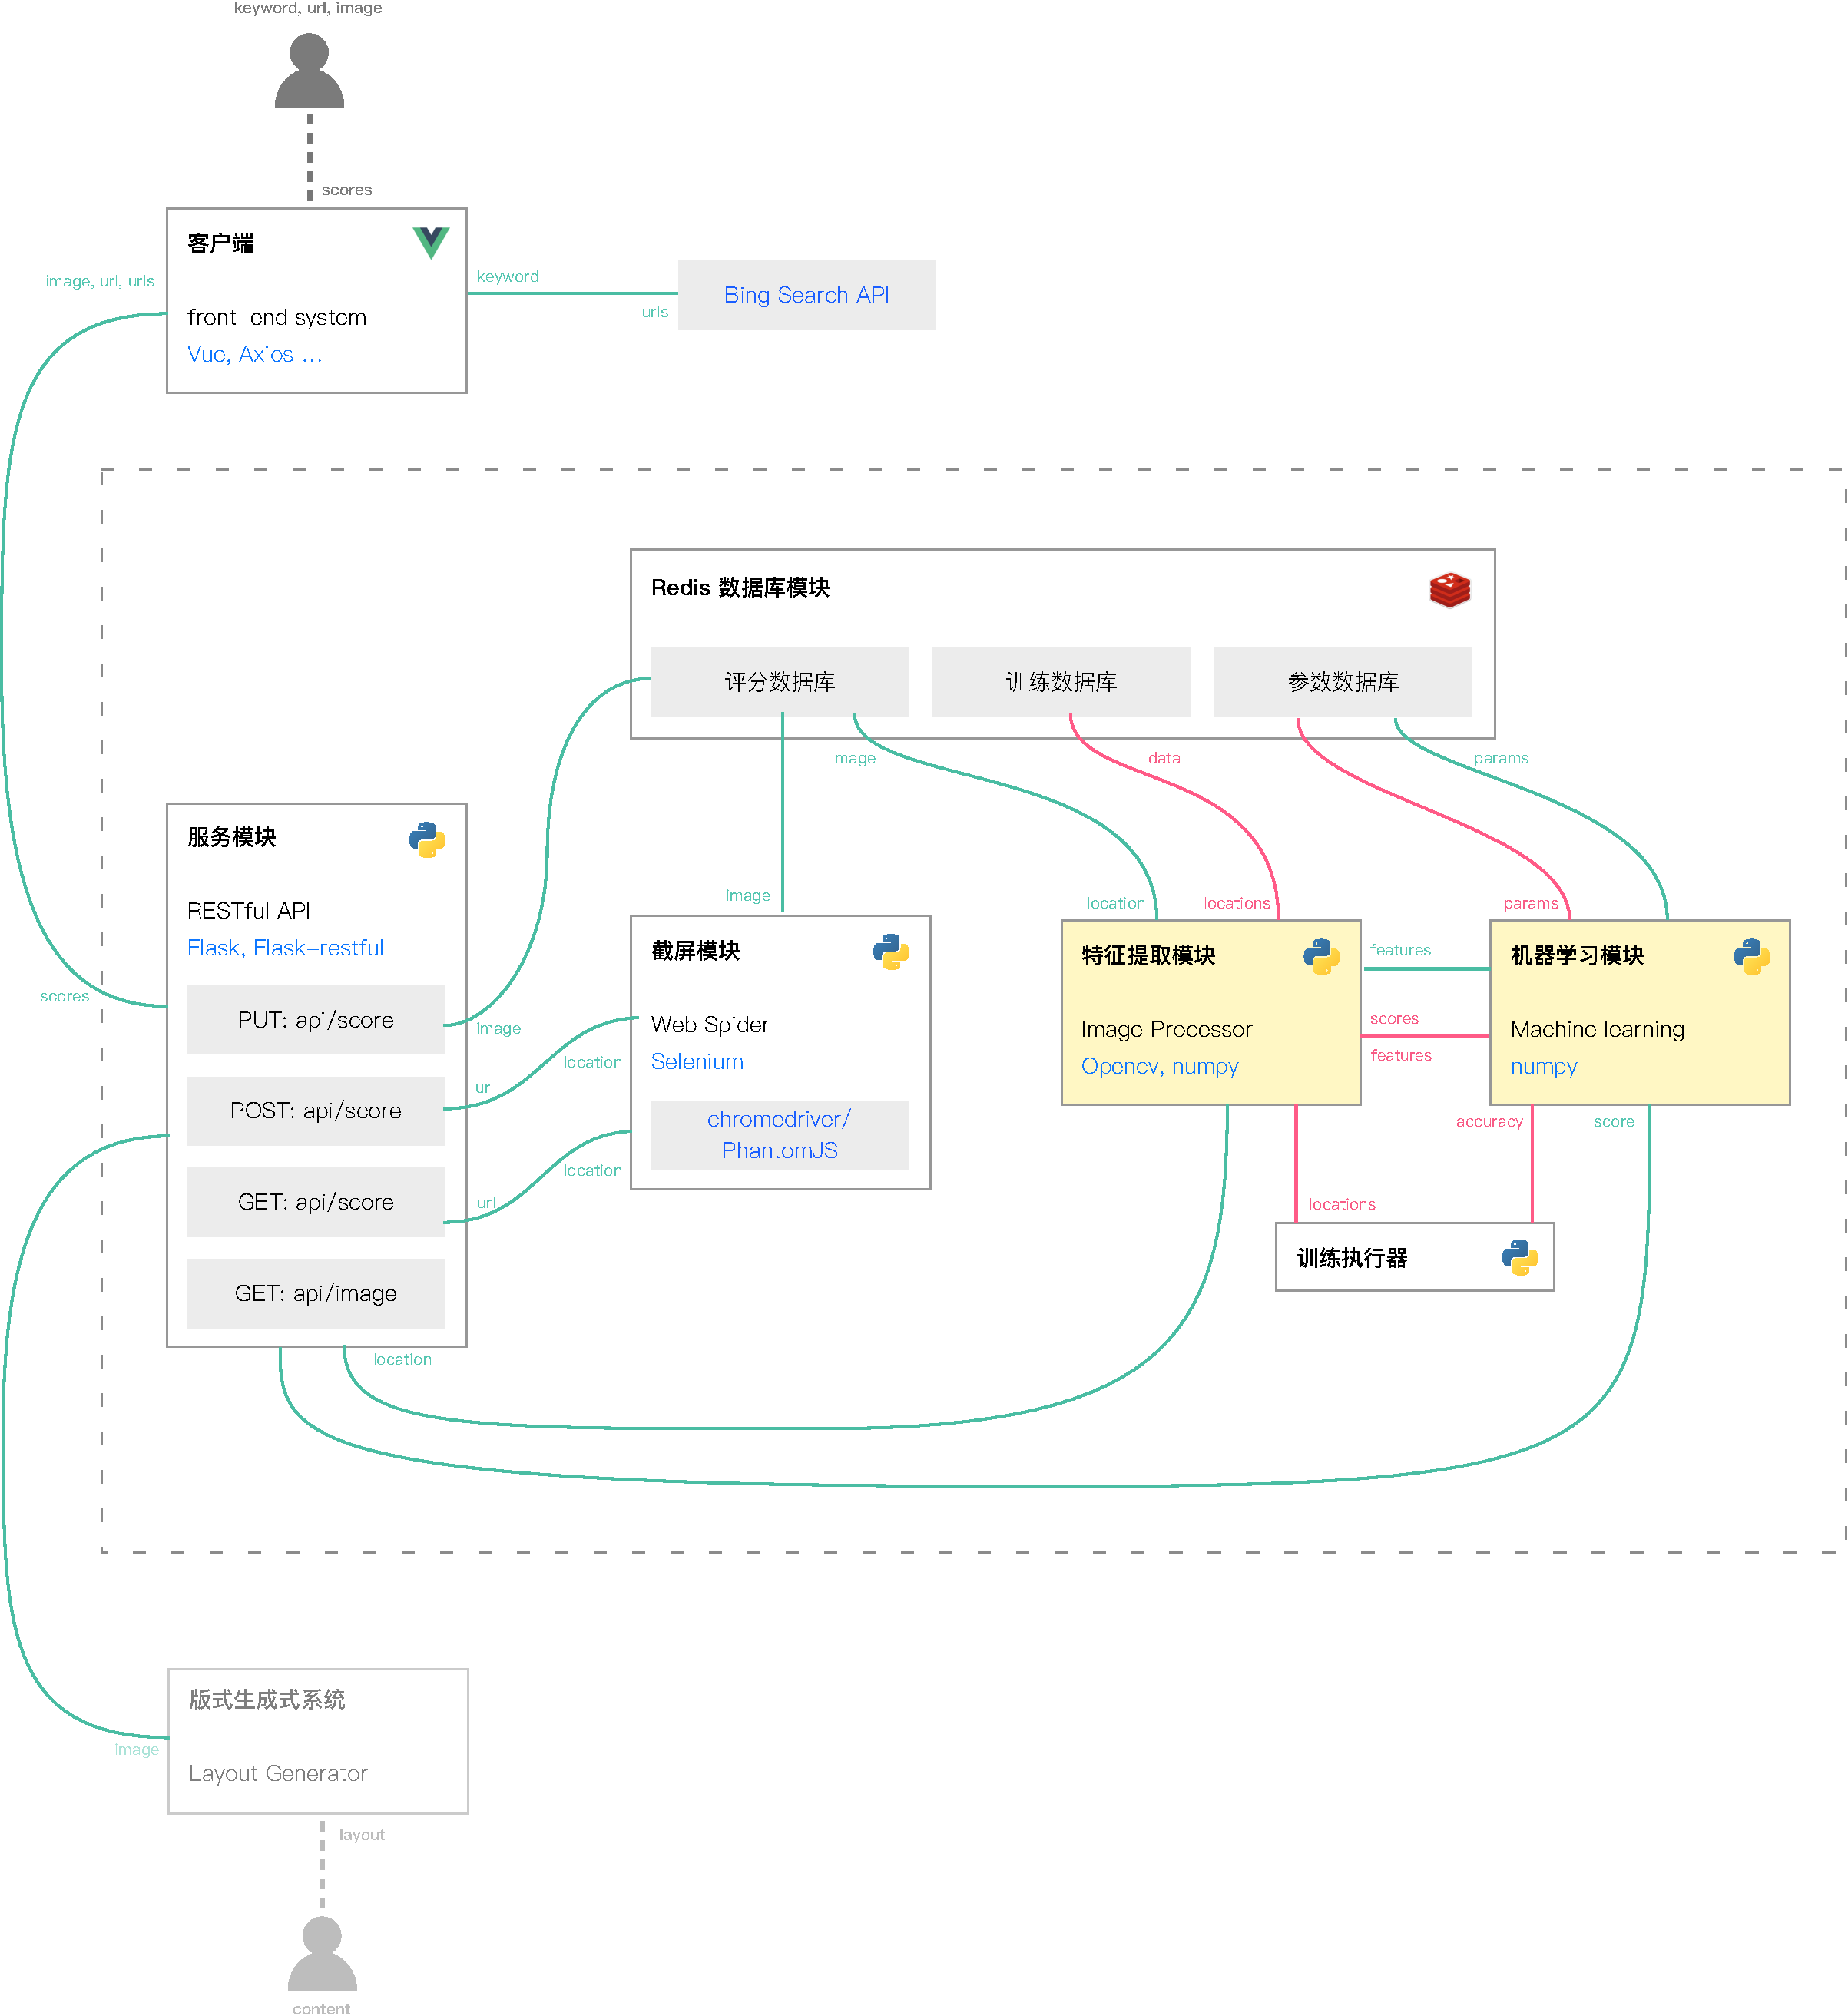
\includegraphics[width=\columnwidth]{fig/fig_sys_structure.pdf}
  \bicaption[fig:sys_struct]{评分系统的模块化架构}{评分系统的模块化架构,图解见图\ref{fig:sys_instruct}}{Fig}{the modular structure of the evaluating system}
\end{figure}

\section{技术架构}
\label{sec:app-tech}

\subsection{模块化设计}

软件工程的模块化设计(Modular Design)是通过把系统划分成可以在不同系统中独立复用的模块(Modules)的设计模式。这些模块构成图状结构,在系统中仅仅通过约定好的接口(Interfaces)进行数据交换。模块化设计可以提高代码的复用率、提高系统对维护开发等过程造成的变化的适应能力\cite{Baldwin2000}。

\begin{figure}[H]
  \centering
  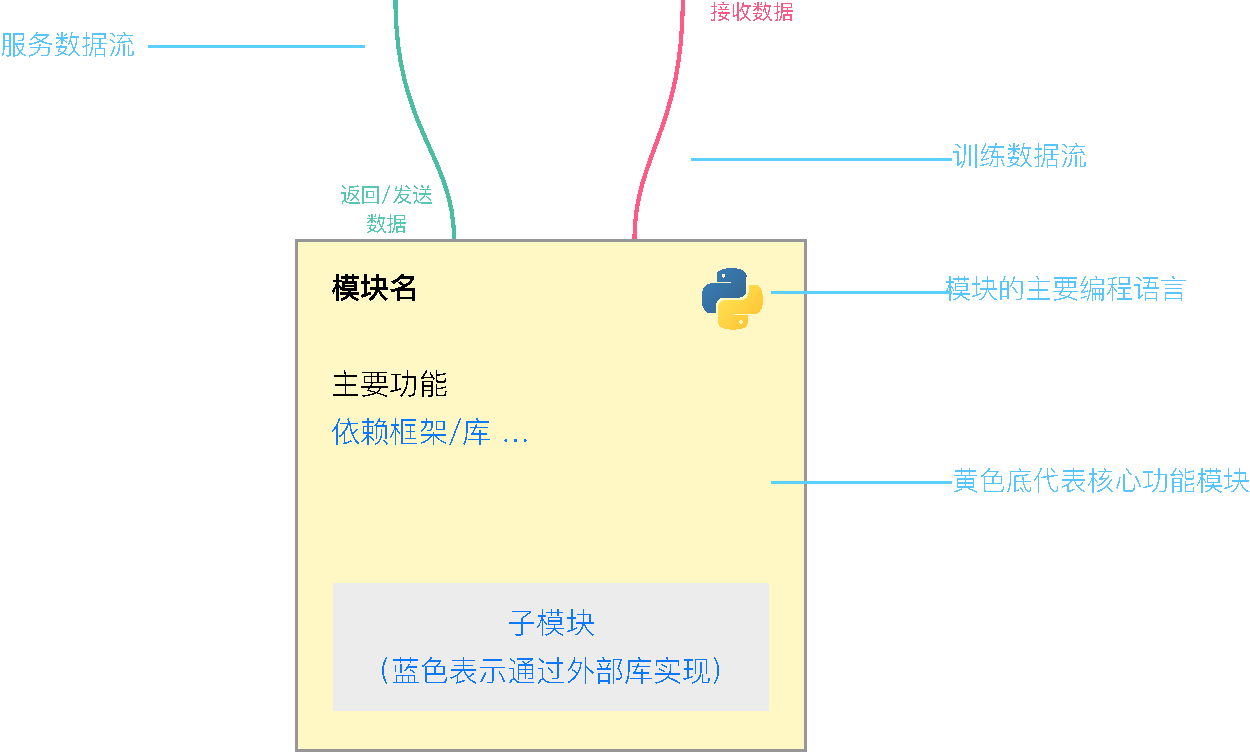
\includegraphics[width=0.6\columnwidth]{fig/fig_struct_instruction.pdf}
  \bicaption[fig:sys_instruct]{评分系统的模块图解}{评分系统的模块图解}{Fig}{the sketch map of a modular}
\end{figure}

图\ref{fig:sys_struct}表现了网页版式评分系统的模块架构。每一个实线矩形代表能够独立实现一项主要功能的模块,图\ref{fig:sys_instruct}说明了这些模块内的文字的含义。虚线矩形内框出的为网页版是美感评分系统,包含了与向外界提供HTTP服务的服务模块;对给定的url进行自动截图的截屏模块;用于管理数据的数据库模块;用于对图像提取特征的特征提取模块,用于进行机器学习的机器学习模块,以及用于驱动训练过程的训练模块。黄色背景的代表系统的核心模块。
虚线框的外部给出了网页版式评分系统的两种应用:上方是一个用户界面模块,展示了用户如何通过用户界面调用评分系统实现网页版式评分相关的需求,如:对关键词的搜索结果按照版式美感排序;上传一张网页图片获得其美感评分等,该模块的功能已经实现。下方是尚未一个实现的网页版式生成式系统,生成式系统可以通过调用评价模块来评价自己生成的网页排版,从而实现生成式的自动化设计,这部分功能尚待实现。

下面通过数据流和模块两部分来具体解释系统的运作方式和采用的技术。

\subsection{数据流}

\subsubsection{服务数据流}
服务数据流描述用户调用评分系统获取评分的过程。以用户对一个输入网页的url以获取网页版式评分的应用场景为例。用户向界面模块输入一个URL,界面模块将URL通过HTTP协议请求报表的形式发送给评分系统的服务模块。服务模块转发数据给截屏模块,截屏模块依照URL对网页进行截图,并将截图交给数据库,数据库储存成功后返还一个标志着截图的存储位置的键(key)给截屏模块,截屏模块转发键给特征提取模块,特征提取模块根据键向数据库获取图片并将提取完的特征向量返还给数据库储存,随后将键交给下游的机器学习模块,机器学习模块根据key向数据库获取特征和学习模型的参数进行评分,将评分一方面存数数据库,一方面返还给服务模块,标志着评分过程的结束。服务模块收到评分后再通过HTTP响应报表将分数发送给界面,界面将分数呈献给用户,就完成了整个服务数据流。

\subsubsection{训练数据流}
训练数据流描述系统内部的参数训过程。训练模块发起训练指令后,特征提取模块读取数据库训练数据集中的数据,开始特征提取,并存数训练数据集。机器学习模块读取这些提取完毕的特征进行模型训练,将训练完毕的模型参数存入数据库中专门的参数模块以供服务数据流调用。除了初始化参数数据库,训练数据流在日常也会不断受到来自外部的训练数据,发起训练过程,迭代更新模型参数以实现与时俱进的评价系统。

\subsection{模块}
\subsubsection{数据库(database)}
依赖:Redis

语言:Python,Redis

为了实现各个模块之间的功能性解耦,所有的模块之间均仅仅通过网页截图计算得到的键(key)来进行沟通,已完成制定的逻辑过程。而每个模块产生的数据,或是计算需要获得的数据都通过一个全局数据库实现读写。

数据采用noSQL的Redis数据库实现,总共划分为评分数据库(Eval\_db),训练数据库(Train\_db)以及参数数据库(Param\_db)三个部分。没个部分的数据通过键值对的嵌套结构进行存储。对于Redis的全部操作通过Python中实现的DB类来实现,包括了简单的增删改查和图像的编码解码等操作。

评分数据库负责缓存客户直接上传或者根据url截屏得到的图片。图片被转成base64编码格式。对base64编码通过哈希SHA1加密算法加密后取前8位,作为该图片保存的键(key)。采用哈希加密作为键的做法有诸多好处。哈希散列是一种对数据改变敏感的加密方式,只要图片数据发生改变,哈希散列就会完全不同。通过哈希散列验证数据是否损坏改变、快速反查上传的图片是否已经在数据库缓存等。图片信息以base64编码字符串的形式存储在数据库中该key下的字典的img字段中(在Redis中被称为哈希Hash)。字典还包含有feature(待计算的特征)字段特征和score字段(待计算的评分)。图\ref{fig:database}展示了存储一张图片内容的键值对的结构。评分数据库中的每个键值对被分别设置了自动释放时间(expire time),在保存24小时后会自动释放空间。

\begin{figure}[H]
  \center
  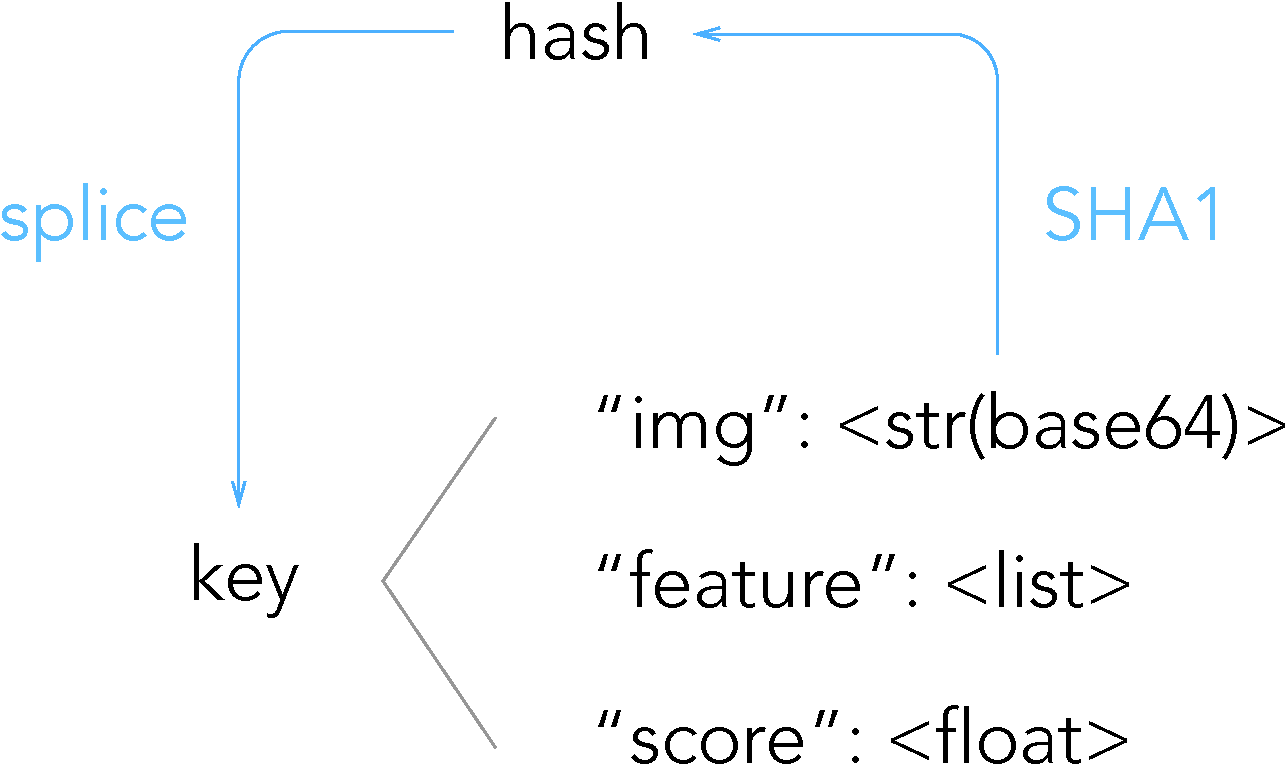
\includegraphics[width=0.4\columnwidth]{fig/fig_database.pdf}
  \bicaption[fig:database]{评分系统数据的键值对结构}{评分系统数据的键值对结构}{Fig}{the key-value hash structure stored in Redis database}
\end{figure}

训练数据库负责存储用于初始机器模型的训练的数据集。以与评分数据库中完全一样的键值对方式进行存储,只是字典中的score字段在初始的时候就已经被标定完毕。训练数据库的所有数据都永久保留,不设置释放时间。

参数数据库的内容很简单,保存了机器模型训练得到的参数。以本文中采用的logistic回归为例,参数以列表的格式存在params字段下。

\subsubsection{服务(server)}
依赖:Flask,Flask-restful

语言:Python

服务模块是与前端的通讯接口,监听前端的请求,并发起系统内部的服务数据流。为了实现对多种请求的响应,服务模块一共开通了如下的4个基于HTTP协议的接口:

\begin{itemize}
  \item 上传url获取评分和键:GET  /api/score
  \item 上传url列表获取评分和键列表:POST  /api/score
  \item 上传图片获取评分和键:PUT  /api/score
  \item 上传键获取图片:GET /api/img
\end{itemize}

实现技术上,服务模块依赖用于快速构建RESTful api的python框架Flask-RESTful。

\subsubsection{截图(screenshot)}

依赖:Selenium,PhantomJS,chromedriver

语言:Python

截图模块接收一个url,获取截图并存入数据库。为了保证网页的渲染效果,通过python爬虫框架Selenium调用chrome浏览器的内核chromedriver进行截屏,亦可调用不会显示浏览器界面的后台虚拟浏览器PhantomJS来截屏,实践表明与chromedriver的渲染效果别无二致。

\subsubsection{特征提取(extractor)}
依赖: cv2,numpy,Pillow

语言:python

特征提取器依照实验二中提取特征的方法进行特征提取并存入数据库。采用图像处理库opencv2和矩阵运算库numpy来实现。特征提取模块通过键向数据库模块获得已经解码完成图像文件,并借助python图形处理库(PIL,此处用Pillow替代)转成Image对象,交由基于opencv2进行图像处理和特征提取的操作。Opencv-pyhton2在数据格式和计算上完全依赖numpy进行,图像处理的关键算法则委托其C++内核进行运算。

\subsubsection{学习与评价(evaluator)}
依赖:Tensorflow,numpy

语言:python

学习与评价模块根据键向数据库获取图像特征和评分(对训练数据流)并进行学习或是评分。学习和评价过程依赖Google开源的Tensorflow机器学习框架实现。Tensorflow意为张量流,结合numpy的矩阵运算和相关模型的数学基础,他可以方便地通过python构建一个学习模型的图,并在外部通过更为底层的语言进行训练和计算,并可进行gpu加速。

\clearpage
\section{小结}
\label{sec:app-sum}
通过对训练集数据按照2:8的验证(Validation)训练(Training)比进行交叉,上述演示系统达到$83\%$的分类准确率。离实际应用尚有一定差距,但一定程度上进一步补充了实验一和实验二关于进化论美学和流畅理论的验证。

%# -*- coding: utf-8-unix -*-
%%==================================================
%% conclusion.tex for SJTUThesis
%% Encoding: UTF-8
%%==================================================

\begin{summary}

本文通过一个眼动实证研究,一个图像特征推测力研究和一个网页版式评分系统的搭建,在理论和应用层面多角度地证实了进化论美学和流畅理论关于视觉复杂度和视觉注意力与美感的关系的猜想。眼动实验提出了视觉注意熵的概念,论证了拥有较强美感的审美对象会导致较小的相对视觉注意熵;图像特征提取实验通过对网格复杂度、占空分布、信息密度分布、视觉显著性分布等特征的提取及验证、论证了网页截图图像中关于视觉复杂度的信息与关于视觉重点分布的特征对美感的显著推测能力;最后,对美感评分系统的具体的工程实现和83\%的网页版式好坏的区分正确率,切实给出了机器获得审美的可行性和技术架构。

上述结论表明,从理论层面上,审美体验遵循最小代价最大收益的原则\citen{Hekkert2006}。“美即是可用”\citen{Tractinsky2000}的观点至少对于先天性的审美而言是正确的。

工程上,网页版式评分系统本身还有诸多值得探索和突破的细节。一个全面而强大的美感评分系统应该是由多个评估模型(如版式、色彩、物件识别、语义等)整合而成的,能对审美对象进行全方位评价的系统。

设计自动化亦是美感评分系统的一个重要的应用方向。基于高效的版式生成式系统和优秀的美感评分系统的生成式设计系统的诞生是令人期待的。然而毋庸置疑,对美学的深入理解和研究是获得高效且优雅\footnote{此处“优雅”指结构清晰可解释}的基石。

\end{summary}


\appendix	% 使用英文字母对附录编号,重新定义附录中的公式、图图表编号样式
\renewcommand\theequation{\Alph{chapter}--\arabic{equation}}
\renewcommand\thefigure{\Alph{chapter}--\arabic{figure}}
\renewcommand\thetable{\Alph{chapter}--\arabic{table}}
\renewcommand\thealgorithm{\Alph{chapter}--\arabic{algorithm}}

%% 附录内容,本科学位论文可以用翻译的文献替代。
\chapter{线上评分页面}
\label{chap:app-survey}

\section{注册及登录界面}
简单起见只要求输入合法的用户名。

\begin{figure}[H]
  \setlength{\fboxsep}{0cm}
  \fbox{
    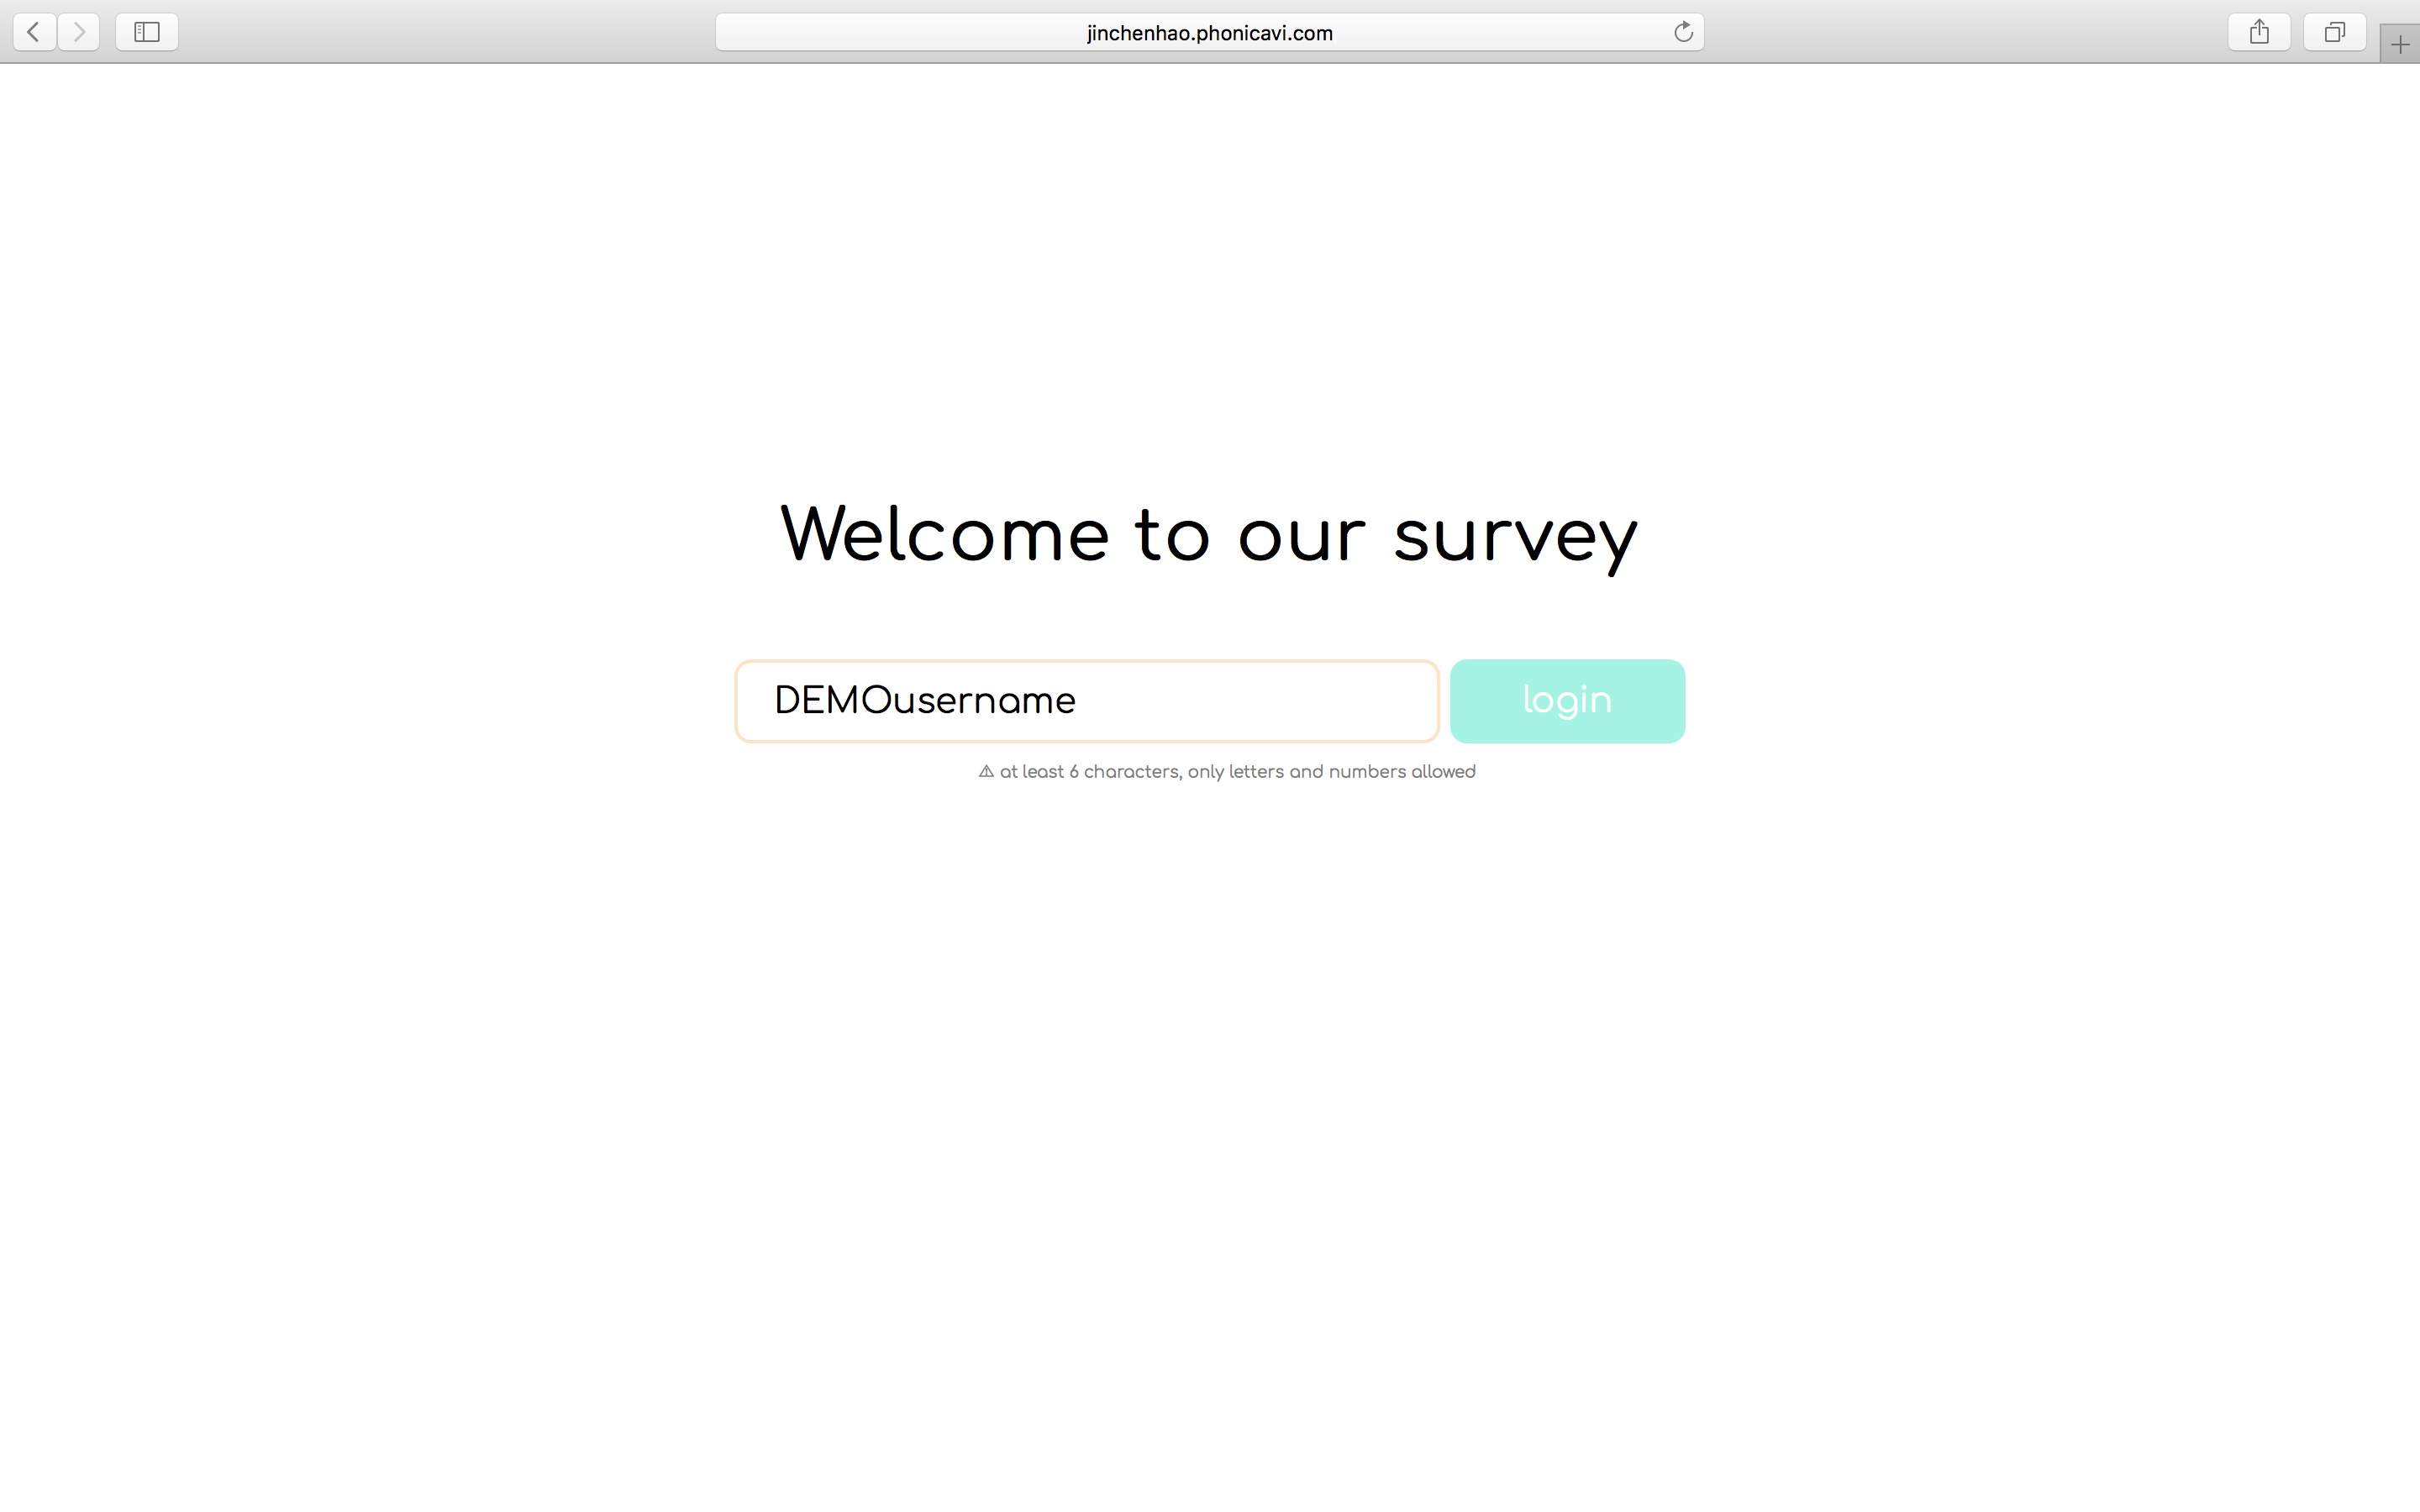
\includegraphics[width = \columnwidth]{fig/fig_app_survey_login.png}
  }
  \bicaption[fig:survey_login]{实验二线上评分登录界面}{第\ref{chap:exp2}章线上评分登录界面}{Fig}{The login page of the online rating}
\end{figure}
\clearpage

\section{说明页面}

\begin{figure}[H]
  \setlength{\fboxsep}{0cm}
  \fbox{
    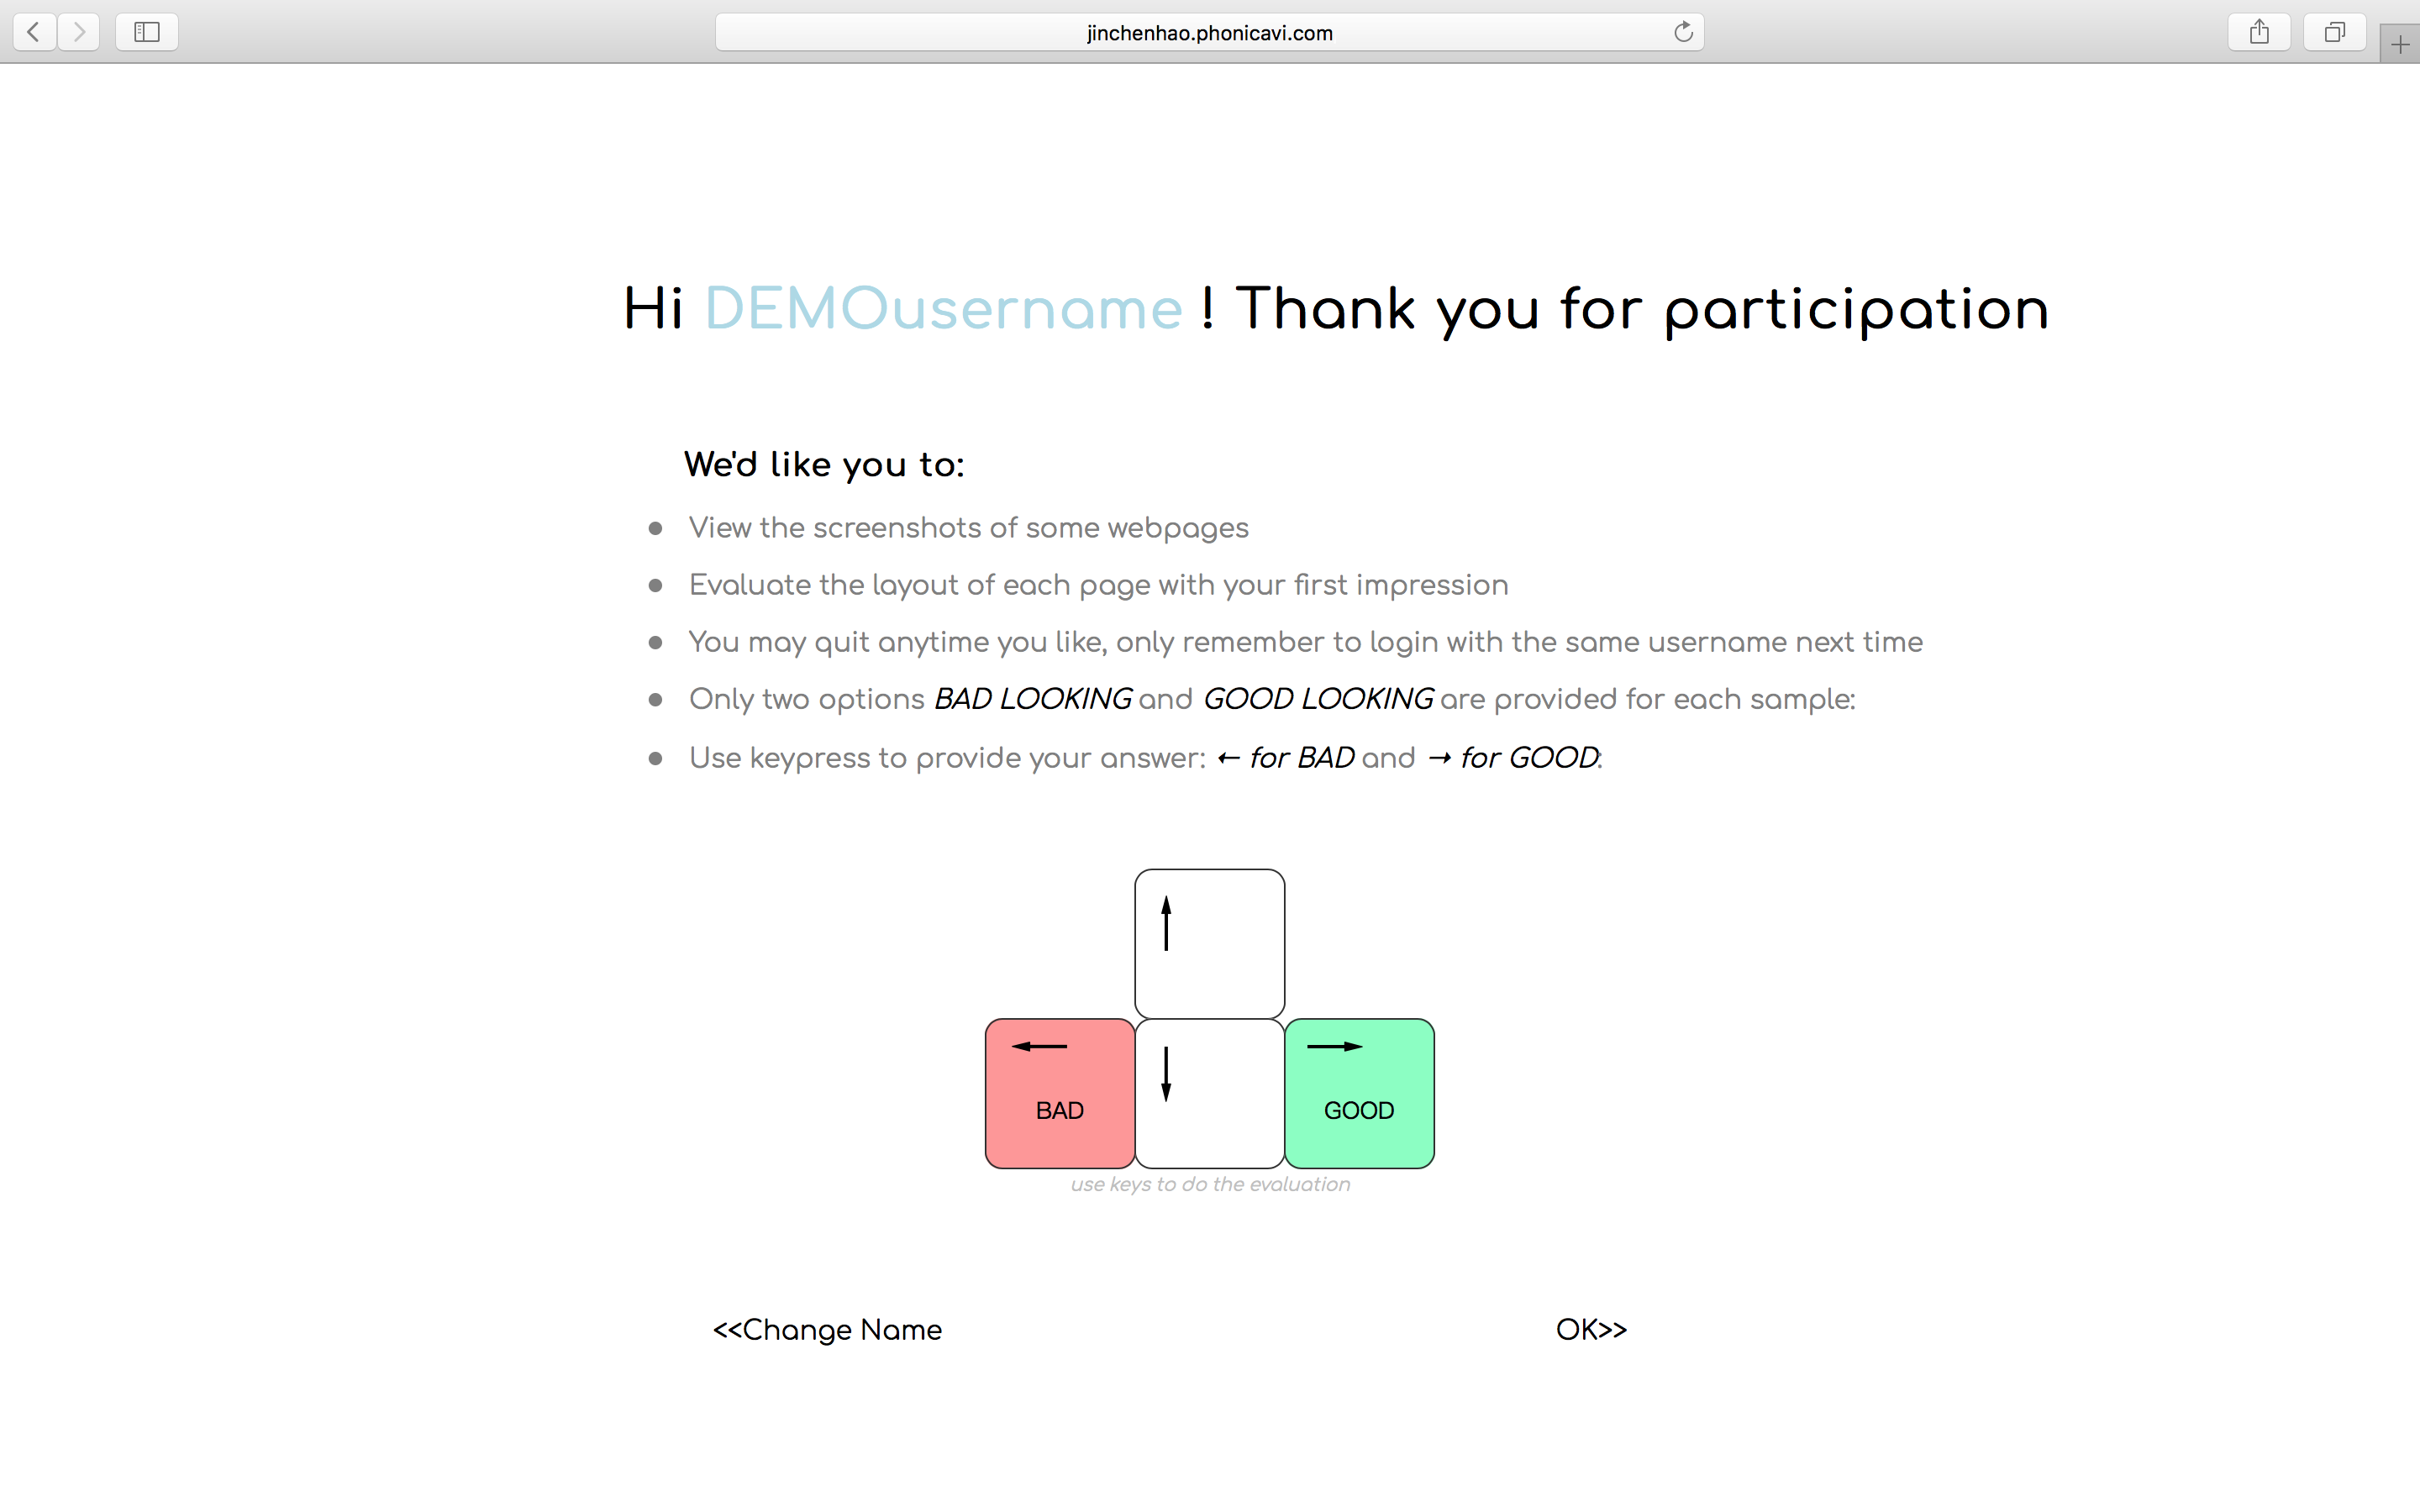
\includegraphics[width = \columnwidth]{fig/fig_app_survey_instruct.png}
  }
  \bicaption[fig:survey_instruction]{实验二线上评分说明界面}{第\ref{chap:exp2}章线上评分说明界面}{Fig}{The instructions page of the online rating}
\end{figure}

\section{评价页面}
由于评价过程中网页截图全屏显示,效果如同直接浏览被评价页面的主页,故不做展示。


\backmatter	% 文后无编号部分

%% 参考资料
\printbibliography[heading=bibintoc]

%% 致谢、发表论文、申请专利、参与项目、简历
%% 用于盲审的论文需隐去致谢、发表论文、申请专利、参与的项目
\makeatletter

%%
% "研究生学位论文送盲审印刷格式的统一要求"
% http://www.gs.sjtu.edu.cn/inform/3/2015/20151120_123928_738.htm

% 盲审删去删去致谢页
\ifsjtu@review\relax\else
  %# -*- coding: utf-8-unix -*-
\begin{thanks}

本文的研究,尤其是眼动实验的相关研究,历时较长。实验期间顾振宇教授长期鼓励和指导,令我有动力去探索更多的解释性指标,并最终取得一定成果。论文撰写上,顾振宇教授的反复修改与指导使结果更为深入和有说服力,令我受益匪浅。

另在实验和工程实现方面,感谢媒设2012级研究生娄坚的特征提取平台;感谢电院2017级研究生邱丰对众包实验平台的搭建上的贡献;感谢电院2017级研究生邓瀚铭对美感评分的机器学习卷积神经网络的搭建;感谢媒设2017级研究生杨秀凡对眼动实验中例外页面的设计改进;感谢媒设2015级研究生张杰琳对代码的重构意见;感谢媒设2015级研究生王靖纯对实验的协助。

感谢所有参与眼动实验和网页众包评分实验的约80名同学和师长。

\end{thanks}
 	  %% 致谢
\fi

\ifsjtu@bachelor
  % 学士学位论文要求在最后有一个英文大摘要,单独编页码
  \pagestyle{biglast}
  \include{tex/end_english_abstract}
\else
  % 盲审论文中,发表学术论文及参与科研情况等仅以第几作者注明即可,不要出现作者或他人姓名
  \ifsjtu@review\relax
    %# -*- coding: utf-8-unix -*-

\begin{publications}{99}
    \item\textsc{第一作者}. {中文非核心期刊论文}, 2017.
\end{publications}

    % \include{tex/projectsreview}
  \else
    %# -*- coding: utf-8-unix -*-
%%==================================================
%% pub.tex for SJTUThesis
%% Encoding: UTF-8
%%==================================================

\begin{publications}{99}
  \item\textsc{金辰浩}. {基于互联网大数据的设计语义模型}[J]. 工业设计, 2017/10(135): 54-55.
  % \item\textsc{Chen H, Wu B~I, Zhang B}, et al. {Electromagnetic Wave Interactions with a Metamaterial Cloak}[J]. Physical Review Letters, 2007, 99(6):63903.
\end{publications}
	      %% 发表论文
    % \include{tex/projects}  %% 参与的项目
  \fi
\fi

% \include{tex/patents}	  %% 申请专利
% \include{tex/resume}	  %% 个人简历

\makeatother

\end{document}
